%% !TeX program = lualatex

%\listfiles	
% **************************
% STOP - Bitte zuerst lesen, bevor Sie weitermachen
%
% Einige Dinge müssen Sie an Ihre Bedürfnisse (und die Vorgaben Ihres
% Betreuers anpassen. Editieren Sie dazu die Datei docinfo.tex).
%
% 1. Sprache
% Das Template unterstützt Deutsch und Englisch, Standard ist Deutsch.
% Wenn Sie Englisch verwenden wollen, ändern Sie bitte direkt am Anfang
% dieser Datei den Eintrag
%    \newcommand{\hsmasprache}{de}
% auf
%    \newcommand{\hsmasprache}{en}
%
% 2. Form der Abgabe
% Das Template unterstützt sowohl eine digitale Abgabe, als auch eine Abgabe
% auf Papier. Bei einer Papierabgabe wird ein doppelseitiger Druck vorbereitet
% und der Titel wird so platziert, dass er in das Fenster des offiziellen
% Umschlages der Hochschule passt.
% Bei einer digitalen Abgabe (als PDF) wird der Titel zentriert und als
% Format wird einseitig gewählt. Außerdem wird die Datei unterschrift.png
% auf dem Blatt mit der Erklärung zur Eigenständigkeit eingebunden.
%
% 3. Zitierstil
% Abhängig von dem gewünschten Zitierstil passen Sie bitte in
% hma.cls die Einstellungen bei \RequirePackage[backend=biber...
% an. Wie ist dort genau erklärt.
% Achtung: Wenn Sie als Zitierstil Fußnoten wählen bzw. generell
% -------  mit Fußnoten arbeiten, dann beachten Sie bitte, dass
%          Fußnoten in Bildunterschriften und Tabellenüberschriften
%          nicht funktionieren.
%          Siehe hierzu https://texfaq.org/FAQ-ftncapt
%          und https://texfaq.org/FAQ-footintab
%          Sinnvollerweise verzichten Sie auf Fußnoten an diesen
%          Stellen und fügen Quellen einfach per \parancite ein.
%
% 4. Doppelseitiger oder einseitiger Druck
% Das Template bestimmt, ob einseitig oder doppelseitig gedruckt wird
% anhand der Abgabeform (papier / digital). Wollen sie dies übersteuern,
% müssen Sie in der Datei preambel.tex folgende Zeile
% \KOMAoptions{twoside=true} für doppelsetigen Druck
% \KOMAoptions{twoside=false} für einsetigen Druck
% direkt vor \usepackage{xcolor} einsetzen. Prinzipiell sollten Sie aber
% das vorgeschlagene Format einfach so lassen.
%
% 5. Unnötige Teile entfernen
% Entfernen Sie die Teile, die Sie nicht brauchen, z.B. Anhänge
%
% 6. Silbentrennung
% LaTeX führt eine automatische Silbentrennung durch. Allerdings
% werden Wörter, die bereits einen Bindestrich enthalten nicht
% getrennt, z.B. Datenschutz-Grundverordnung. Wenn Sie Ihren Text auf
% Deutsch schreiben, können Sie dann alternativ "= für den Bindestrich
% im Wort verwenden, z.B. Datenschutz"=Grundverordnung, damit LaTeX
% weiterhin richtig trennt.
% Ist die Silbentrennung aus einem anderen Grund nicht erfolgt, sodass
% das Wort über den rechten Rand hinaussteht oder wenn Sie eine weitere
% Trennstelle wollen, können Sie LaTeX helfen, indem Sie weitere
% Trennstellen angeben. Dies geschieht durch "- als Zeichen, z.B.
% Staats"-vertrag.
%
% 7. Nummerierung der Fußnoten
% LaTeX beginnt die Nummerierung der Fußnoten in jedem Kapitel wieder
% bei 1. In diesem Template wird die fortlaufende Nummerierung der Fußnoten 
% über die gesamte Arbeit umgesetzt.  
%
% 8. Unterschrift
% Bei einer Abgabe auf Papier unterschreiben Sie die Arbeit eigenhändig.
% Geben Sie allerdings digital ab, sollten Sie die Datei unterschrift.png in dem 
% Ordner /bilder durch einen Scan Ihrer eigenen Unteschrift ersetzen - andernfalls
% unterschreiben Sie als Max Mustermann ;-)
% *******************************************************************

% -------------------------------------------------------
% Informationen und Einstellungen für Ihre Abschlussarbeit
%

% Sprache für das Dokument festlegen
\newcommand{\hsmasprache}{en} %de für Deutsch oder en für Englisch


% Abgabeform festlegen
% Bei einer digitalen Abgabe, wird das Dokument einseitig erzeugt und der Titel wird
% zentriert.
\newcommand{\hsmaabgabe}{digital} % Abgabe erfolgt für Fakultät I digital. Optionen hier sind für anderen Fakultäten: "papier" oder "digital".


% Flags für Veröffentlichung, Sperrvermerk
\newcommand{\hsmapublizieren}{opensource}   
% Wird einer Veröffentlichung zugestimmt?
% Optionen: 
% opensource = Druck der CC Lizenz mit By SA (Standard)
% hs = Veröffentlichung an der Hochschule und auf Hochschulservern
% stud = kein opensource und keine veröffentlichung auf den Hochschulservern
% vertraulich = Arbeit darf nicht veröffentlicht werden und erhält einen Sperrvermerk (Nur nach Absprache mit Betreuer setzen!)


\newcommand{\genderhinweis}{gender}     % Soll der Gender-Hinweis angezeigt werden? ja=gender, nein = nogender; Genderhinweis wird nur in deutscher Sprache angezeigt!


\newcommand{\hsmaquellcode}{sourcecode} % Verwenden Sie Quellcode in Ihrer Arbeit? ja=sourcecode, nein= nosourcecode

\newcommand{\hsmasymbole}{symbole} % Verwenden Sie viele Symbole in Ihrer Arbeit, welche in einem Symbolverzeichnis aufgeführt werden sollen? ja=symbole, nein= nosymbole


\newcommand{\hsmaglossar}{noglossar} % Verwenden Sie Begriffserklärungen nicht Abkürzungen in Ihrer Arbeit? ja=glossar, nein= noglossar

\newcommand{\hsmatc}{tc} % Verwenden der Änderungsmarkierung. Änderungsmarkierung aktiv und eine Liste der Änderungen wird angezeigt = tc, Keine Änderungsmarkierung und keine Ausgabe der Änderungen = notc




% Titel der Arbeit auf Deutsch
\newcommand{\hsmatitelde}{Fine-tunen kleiner Sprachmodelle zur Code-Synthese auf Funktionsebene}

% Titel der Arbeit auf Englisch
\newcommand{\hsmatitelen}{Fine-tuning small language models for code synthesis on a function level}

% Weitere Informationen zur Arbeit
\newcommand{\hsmaort}{Mannheim}          % Ort
\newcommand{\hsmaautorvname}{Jan}        % Vorname(n)
\newcommand{\hsmaautornname}{Diekhoff}   % Nachname(n)
\newcommand{\hsmaabgabedatum}{2024-11-07}% Datum der Abgabe in dem Format JJJJ-MM-TT

\newcommand{\hsmafirma}{} % Firma bei der die Arbeit durchgeführt wurde
\newcommand{\hsmabetreuer}{Prof. Dr. Jörn Fischer} % Betreuer an der Hochschule
\newcommand{\hsmazweitkorrektor}{Prof. Dr. rer. nat. Kai Eckert}   % Betreuer im Unternehmen oder Zweitkorrektor

\newcommand{\hsmafakultaet}{I}    % I für Informatik oder E, S, B, D, M, N, W, V
\newcommand{\hsmastudiengang}{IM} % IB IMB UIB CSB IM MTB (weitere siehe studiengaenge.tex)

% Dokumententyp, benutzte Pakete und deren Einstellungen
\documentclass[	\hsmasprache,%
				\hsmaabgabe,%
				\hsmapublizieren,%
				\genderhinweis,
				\hsmaquellcode,
				\hsmasymbole,
				\hsmaglossar,
				\hsmatc]{HMA}

% Wo sind die Bilder?
\graphicspath{{bilder/}}


% Wo liegt Sourcecode?
\newcommand{\srcloc}{src/}


% Checklisten mit zwei Ebenen
\newlist{checklist}{itemize}{2}
\setlist[checklist]{label=$\square$}



% Befehl zum Erstellen eigener Makros. In diesem Fall ist es ein Makro für das Einbinden von Bildern. Das label (für \ref) ist dann der Name der Bilddatei
\newcommand{\bild}[3]{
	\begin{figure}[ht]
		\centering
		\includegraphics[width=#2]{#1}
		\caption{#3}
		\label{#1}
\end{figure}}




							


\newcommand{\snowcard}[9]{
	\begin{table}[ht!]
		\caption{\hsmasnowcardanforderung\ #1 -- #4}\label{#1}
		\renewcommand{\arraystretch}{1.2}
		\centering
		\sffamily
		\begin{footnotesize}

			\begin{tabularx}{\linewidth}{sssssl}
				\toprule
				\textbf{\hsmasnowcardno} & #1 & \textbf{\hsmasnowcardart} & #2 & \textbf{\hsmasnowcardprio} & #3 \\
				\midrule
				\multicolumn{2}{l}{\textbf{\hsmasnowcardtitel}} & \multicolumn{4}{l}{\parbox[t]{11.8cm}{#4}} \\
				\ifx&#5&%
				\else
				\multicolumn{2}{l}{\textbf{\hsmasnowcardherkunft}} & \multicolumn{4}{l}{\parbox[t]{11.8cm}{#5}} \\
				\fi
				\ifx&#6&%
				\else
				\multicolumn{2}{l}{\textbf{\hsmasnowcardkonflikt}} & \multicolumn{4}{l}{\parbox[t]{11.8cm}{#6}} \\
				\fi
				\addlinespace
				\multicolumn{6}{l}{\textbf{\hsmasnowcardbeschreibung}} \\
				\multicolumn{6}{l}{\parbox[t]{13.5cm}{#7\strut}} \\
				\ifx&#8&%
				\else
				\addlinespace
				\multicolumn{6}{l}{\textbf{\hsmasnowcardfitkriterium}} \\
				\multicolumn{6}{l}{\parbox[t]{13.5cm}{#8\strut}} \\
				\fi
				\ifx&#9&%

				\else
				\addlinespace
				\multicolumn{6}{l}{\textbf{\hsmasnowcardmaterial}} \\
				\multicolumn{6}{l}{\parbox[t]{13.5cm}{#9\strut}} \\
				\fi
				\bottomrule
			\end{tabularx}
		\end{footnotesize}
	\end{table}
}



% Quality Attribute Scenario
\newcommand{\qas}[9]{
	\begin{table}[ht!]
		\caption{\hsmaqasanforderung\ #1 -- #3}\label{#1}
		\renewcommand{\arraystretch}{1.2}
		\centering
		\sffamily
		\begin{footnotesize}

			\begin{tabularx}{\linewidth}{sssssl}
				\toprule
				\textbf{\hsmaqasno} & #1 & \textbf{\hsmaqasart} & QAS & \textbf{\hsmaqasprio} & #2 \\
				\midrule
				\multicolumn{2}{l}{\textbf{\hsmaqastitel}} & \multicolumn{4}{l}{\parbox[t]{11.8cm}{#3}} \\
				\multicolumn{2}{l}{\textbf{\hsmaqasquelle}} & \multicolumn{4}{l}{\parbox[t]{11.8cm}{#4}} \\
				\multicolumn{2}{l}{\textbf{\hsmaqasstimulus}} & \multicolumn{4}{l}{\parbox[t]{11.8cm}{#5}} \\
				\multicolumn{2}{l}{\textbf{\hsmaqasartefakt}} & \multicolumn{4}{l}{\parbox[t]{11.8cm}{#6}} \\
				\addlinespace
				\multicolumn{6}{l}{\textbf{\hsmaqasumgebung}} \\
				\multicolumn{6}{l}{\parbox[t]{13.5cm}{#7\strut}} \\
				\addlinespace
				\multicolumn{6}{l}{\textbf{\hsmaqasantwort}} \\
				\multicolumn{6}{l}{\parbox[t]{13.5cm}{#8\strut}} \\
				\addlinespace
				\multicolumn{6}{l}{\textbf{\hsmaqasmass}} \\
				\multicolumn{6}{l}{\parbox[t]{13.5cm}{#9\strut}} \\
				\bottomrule
			\end{tabularx}
		\end{footnotesize}
	\end{table}
}

\newcommand{\acf}[1]{\acrfull{#1}}
\newcommand{\acl}[1]{\acrlong{#1}}
\newcommand{\ac}[1]{\gls{#1}}
\newcommand{\acs}[1]{\acrshort{#1}}
\newcommand{\acp}[1]{\glspl{#1}}
\newcommand{\Ac}[1]{\Gls{#1}}
\newcommand{\Acp}[1]{\Glspl{#1}}
\newcommand{\Acf}[1]{\Acrfull{#1}}
\newcommand{\Acs}[1]{\Acrshort{#1}}


\usepackage{pgfplots}
\usepackage{tikz}
\usepackage{filecontents}
\usepackage{array}
\usepackage{geometry}
\usepackage{multirow,multicol,booktabs}
\usepackage{float}

\usepgfplotslibrary{colorbrewer}
\pgfplotsset{cycle list/Set2-8}
\pgfplotsset{compat=1.17}

\usepackage{listofitems} % for \readlist to create arrays
\tikzstyle{mynode}=[thick,draw=black,fill=white,circle,minimum size=22]

\usepackage{algorithm}
\usepackage{algpseudocode}

\usepackage{svg}
% -------------------------------------------------------
% Abstrakt / Abstract
% Achtung: Wenn Sie im Abstrakt Anführungszeichen verwenden wollen, dann benutzen Sie
%          nicht "` und "', sondern \enquote{}. "` und "' werden nicht richtig
%          erkannt.

% Kurze (maximal halbseitige) Beschreibung, worum es in der Arbeit geht auf Deutsch
\newcommand{\hsmaabstractde}{Code-Synthese-Sprachmodelle sind Sprachmodelle, welche Code generieren können.
Ihre Entwicklung ist ein rasch wachsendes Forschungsfeld.
Diese Arbeit stellt die TinyFunc-Coder-Modelle vor, eine Reihe von Code-Synthese-Modellen, die als Proof of Concept für eine Lernhilfe für Studenten der Hochschule Mannheim zum Umgang mit künstlicher Intelligenz beim Programmieren dienen soll.
Anstatt auf bestmögliche Performanz trainiert zu sein, erfüllt sie eine spezifische Rolle, in der sie nur auf spezifische Anforderungen antworten können soll, nämlich das Generieren von Funktionskörpern auf Eingabe eines Funktionskopfes und Docstrings.
Diese These stellt ebenfalls TinyFuncData vor, ein Datensatz von 6,4M Reihen an Funktionsdefinitionen, die aus dem The Stack-Datensatz extrahiert wurden.
Aufgrund von Zeit- und Hardware-Einschränkungen wurden viele Optimierungstechniken beim Weitertrainieren der Modelle eingesetzt.
Bei der Evaluierung auf einem großen Problemsatz, der hauptsächlich aus Problemen des Bigcode Evaluation Harness besteht, erziehlt TinyFuncCoder keine wesentlich besseren Ergebnisse als TinyLlama.
Dies liegt sowohl an Entscheidungen im Trainingsprozess als auch an den Einschränkungen, unter denen trainiert wurde.
Dies bietet viel Spielraum für weitere Forschung zum Erschaffen eines Modells, dass die Anforderungen an TinyFuncCoder erfüllt.
}

% Kurze (maximal halbseitige) Beschreibung, worum es in der Arbeit geht auf Englisch
\newcommand{\hsmaabstracten}{Code synthesis models are language models which can generate code. 
Their development is a rapidly growing field of research.
This thesis introduces a series of code synthesis language models -- the TinyFuncCoder models -- intended to be a proof of concept for a learning aide for students of the University of Applied Sciences of Mannheim to learn to write code assisted by language models.
Rather than aiming for state-of-the-art performance, they intend to fulfill a specific, niche role and task by only being capable of generating function bodies when prompted with a function head and docstring.
Further, this thesis introduces TinyFuncData, a 6.4M row dataset containing function definitions for ten programming languages filtered from The Stack dataset.
The models are fine-tuned from the TinyLlama series using many parameter-efficient fine-tuning techniques due to time and resource restrictions.
Evaluating on a large evaluation set comprised mainly of the Bigcode Evaluation Harness, the TinyFuncModels are not significantly better than the base TinyLlama models due to decisions made during model creation and a lack of training impact due to tradeoffs made because of restrictions.
This leaves much room for further work to create a code synthesis model that fulfills the desired capabilities of TinyFuncCoder.}

\addbibresource{literatur.bib}


\begin{document}	
\newacronym{adam}{Adam}{adaptive moment estimation}
\newacronym{ai}{AI}{artificial intelligence}
\newacronym{ast}{AST}{abstract syntax tree}
\newacronym{cot}{CoT}{chain of thought}
\newacronym{dora}{DoRA}{weight-decomposed low-rank adaptation}
\newacronym{fnn}{FNN}{feedfoward neural network}
\newacronym{gpt}{GPT}{generative pre-trained transformer}
\newacronym{gpu}{GPU}{graphical processing unit}
\newacronym{icl}{ICL}{in-context learning}
\newacronym{llm}{LLM}{large language model}
\newacronym{lm}{LM}{language model}
\newacronym{lora}{LoRA}{low-rank adaptation}
\newacronym{mbpp}{MBPP}{Mostly Basic Programming Problems}
\newacronym{ml}{ML}{machine learning}
\newacronym{nlg}{NLG}{natural language generation}
\newacronym{nlp}{NLP}{natural language processing}
\newacronym{nlu}{NLU}{natural language understanding}
\newacronym{peft}{PEFT}{parameter-efficient fine-tuning}
\newacronym{qlora}{QLoRA}{quantized low-rank adaptation}
\newacronym{qdora}{QDoRA}{quantized weight-decomposed low-rank adaptation}
\newacronym{regex}{regex}{regular expression}
\newacronym{rnn}{RNN}{recurrent neural network}
\newacronym{relu}{ReLU}{rectified linear unit}
\newacronym{wsl}{WSL}{Windows subsystem for Linux}

%\begin{acronym}[NLP]
%    \acrodef{nlp}[NLP]{Natural Language Processing}
%\end{acronym}

% Glossareinträge
\newglossaryentry{glos:amplification}{name={Amplification}, description={describes the disproportionate increase of a response packet compart to the initial request packet.}}

% Verzeichnis von Symbolen und Einheiten
\newglossaryentry{symb:Pi}{name=\ensuremath{\pi},
	description={Geometrical value},
	unit={},
	type=symbolslist}

\newglossaryentry{symb:energyconsump}{name=\ensuremath{P},
	description={Energy consumption},
	unit={\si{kW}},
	type=symbolslist}
	
\pagestyle{headings}
\tableofcontents


\mainmatter
\chapter{Introduction}
\label{chap:intro}

This thesis will introduce the TinyFuncCoder series, a collection of \acp{lm} trained to synthesise code purely from function heads and docstrings. It further itnroduces the TinyFuncData dataset used to train it.
Section \ref{sec:motivation} will introduce the motivation for creating this series of models, as well as the research questions this thesis aims to answer.
Section \ref{sec:overview} will provide an overview of the structure of the thesis.

\section{Motivation and Research Goals}
\label{sec:motivation}

The TinyFuncCoder models aim to be \acp{lm} that can synthesise code.
Code synthesis models are not unique to this thesis, as presented in chapter \ref{sec:synthmodels}.
However, TinyFuncCoder will be exclusively trained on function definitions and thus should only generate functions without further comments, class structures or other information.
Its intended use is to be fed a function signature and produce the function body from this information.
This thesis uses the term \emph{function signature} to mean a function head including the name, return type and parameters, as well as a docstring. The term \emph{function definition} refers to a signature and its corresponding function body.

TinyFuncCoder aims to be a proof of concept for an in-house \ac{lm} that can help students of the University of Applied Sciences Mannheim learn the use of \acp{lm} when coding in a controlled environment.
The name comes from TinyLlama, the base model used for training, and a shortened \enquote{function coder}.
As \ac{lm}-assisted coding becomes more commonplace, it is an important skill to learn to properly utilize them.
As such, TinyFuncCoder's purpose is to be a bare-minimum coding model that can help fill out simple function bodies while still forcing students to think about which functions they need for their use case and plan the architecture of their code.
Coding with a general-purpose \ac{llm}, most commonly ChatGPT, allows skipping this step by simply asking a plain-language query.
To prevent this, TinyFuncCoder is not intended to understand plain-language queries.
It will also not support infilling or bugfixing as these are more advanced, complicated behaviours for a code synthesis \ac{lm}.

Ideally, TinyFuncCoder can serve as the basis for a model that can be used in classrooms or even exams without concerns of trivialising challenges or disrupting the learning process.
It should only produce results when queried properly because of its custom tuning, and it should run on most devices and can be further tuned easily on available university hardware due to its small size.
It should be usable without requiring an internet connection, potentially enabling its use even during an exam for classes where its use has been established.

The main question which this thesis aims to answer is \emph{How well can a \acl{lm} be fine-tuned to only synthesise function bodies from their signature?}
This question assumes that fine-tuning \acp{lm} for code synthesis is possible, and this thesis will showcase many examples of this.
The novel approach of this thesis is using only function definitions for fine-tuning.
To the best of our knowledge, other code synthesis models utilize various approaches to create their data for code synthesis fine-tuning, but none utilize a dataset of only function definitions.
Because this question is explored in the constraints of a Master's thesis, certain restrictions apply that limit the possible scope of research.
First, the available time is six months.
Because research, coding, dataset creation and evaluation all take up time in which training cannot simultaneously occur, the available time to train TinyFuncCoder is limited to three months at best.
Second, many state-of-the-art code synthesis models are trained on very powerful and costly hardware that is not available within the scope of this thesis.
Most of the code is run on a server of the University of Applied Sciences Mannheim or on a private machine, as further detailed in section \ref{sec:hardware}.
This hardware limitation in turn influences which size range of model can be used for fine-tuning and how long fine-tuning takes.
Taking these into account, a more precise research question is
\begin{quote}
\emph{How well can a small \acl{lm} be fine-tuned to only synthesise function bodies from a function signature using limited hardware?}
\end{quote}
It can be expected that the TinyFuncCoder series will not be able to compete with state-of-the-art models, so this thesis explores how much performance can be achieved under the given restrictions.

The following subquestions should also be considered when answering the main question:

\paragraph{Which \ac{lm}(s), should be used as base models for fine-tuning?}
The chosen model(s) for fine-tuning need to meet multiple requirements to be viable.
They need to be open-source and have a permissive license for further training without any royalties or other usage requirements.
They need to be small enough to be able to be fine-tuned on the available hardware, but still good enough to merit consideration.
Being pre-trained on code can be both a benefit and a hindrance.
If they have been already trained on code, it will presumably be easier to strengthen this knowledge, but it may also utilize knowledge that falls outside of the scope of TinyFuncCoder.

\paragraph{How can the coding ability of a \ac{lm} be judged?}
To see if TinyFuncCoder can fulfill its purpose, its code synthesis abilities need to be assessed on some metric.
Do one or more appropriate metrics already exist or does one need to be devised?


\section{Overview}
\label{sec:overview}

Chapter \ref{chap:nlp} explains the fundamental knowledge required to understand this thesis, including basic \ac{nlp} and \ac{ml} concepts, as well as more specialized approaches like \ac{qlora} used for TinyFuncCoder.
It also introduces the Starcoderdata dataset that will be used as a base for this thesis' TinyFuncData dataset, and the evaluation metrics that will be applied to assess TinyFuncCoder's proficiency in code synthesis.
Chapter \ref{chap:related} presents other approaches to creating code synthesis datasets and models, showcasing their unique approaches, advantages and disadvantages.

Chapter \ref{chap:tinycoder} presents the contributions made by this thesis, including creating the dataset, setting up the model, training and evaluation architecture, and the exploratory training tests done.

Chapter \ref{chap:results} showcases TinyFuncCoder's performance on various metrics.
Chapter \ref{chap:discussion} discusses these results and the work done as a whole.
Chapter \ref{chap:conclusion} acts as a recap and summary of everything presented.
\chapter{Fundamentals}
\label{chap:nlp}

This chapter presents the fundamental knowledge necessary to understand the work and research done for this thesis.
Section \ref{sec:nlp} explains \ac{nlp} concepts like \acp{fnn}, training and optimization, tokenization, the transformer architecture and \ac{peft} techniques.
Section \ref{sec:metrics} presents various popular metrics used to evaluate code synthesis \acp{lm}.
Section \ref{sec:thestack} introduces the The Stack dataset, the basis for the TinyFuncData dataset created by this thesis.
Finally, section \ref{sec:basemodels} explores possible models that could serve as the base for TinyFuncCoder.

\section{Natural Language Processing}
\label{sec:nlp}
\Ac{nlp} is a field that has received much public attention since its inception.
From early chatbots like ELIZA \cite{Weizenbaum.1966} to Amazon's Alexa \cite{Kumar.2017}, Google Translate \cite{Wu.2016} or the recent breakthroughs in \acp{lm} like the ubiquitous transformer architecture \cite{Vaswani.2017} in 2017 and OpenAI's ChatGPT \cite{OpenAI.2022,AlecRadfordKarthikNarasimhanTimSalimansIlyaSutskever.2018,Brown.2020} in 2022.
\ac{nlp} has a vast amount of use cases, including content filters, text analysis, completion and prediction or translation.
Most relevant for this thesis is its use in code synthesis.
In essence, \ac{nlp} is a field of study in which computers learn to interact with natural language, as opposed to structured language like code.
It can be broadly split into \ac{nlu} and \ac{nlg}, the first of which processes natural language into an internal representation, and the second processes internal representations into natural language based on an input.

\subsection{History of NLP}
\label{sec:history}
The field of \ac{nlp} has existed since the 1950's, with three major epochs.
Symbolic \ac{nlp}, starting in the 50's \cite{Nadkarni.2011,Johri.2021}, working mostly with sets of hand-written rules and being rather limited in scope.
With Chomsky's introduction of syntactic structures \cite{Lees.1957}, computers could process simple phrases.
While many developments in the field had impressive capabilities for the time, it became apparent that natural language could not easily be captured in a structured language.
Natural language has a very large vocabulary and is ambiguous and reliant on context to process.

With ever-increasing computer processing power and the invention of \ac{ml}, \ac{nlp} adopted a statistical approach in the 90's \cite{Nadkarni.2011}.
It replaced the rigid rules of the symbolic method with statistical models that would predict the most likely word based on a previous series of words.
Models were trained on large bodies of annotated text \cite{Nadkarni.2011,Manning.1999}, utilizing the \ac{ml} practice of supervised learning.

This \ac{ml} approach was strengthened with the adoption of deep learning and neural networks.
In 2003, Bengio et al. introduced the foundation for most current \ac{nlp}, creating a neural model that handily outperformed the $n$-gram model, the best model at the time \cite{Bengio.2003}.
More recent advancements will be discussed in their own upcoming sections.

\subsection{Machine Learning Fundamentals}
\label{sec:ml}
This section will provide a brief overview of the underlying \ac{ml} concepts of current \ac{nlp} architecture, the \ac{fnn} and how optimizers are used in its training.

\subsubsection{Feedforward Neural Networks}
\label{sec:fnn}
A \ac{fnn}, broadly, is a collection of interconnected artificial neurons through which data flows and is processed.
An artificial neuron, inspired by a biological neuron, consists of a set of operations done on an input.
As shown in figure \ref{fig:neuron}, it consists of an input vector $x$, a weight vector $w$, an optional bias $b$, and an activation function $f$.
The neuron sums the product of all $x_i$ with their respective $w_i$ and adds $b$, then passes the result into $f$ \cite{Jurafsky.2024}.
The activation function has a large impact on the output, as it determines how the calculated sum is processed.
Common functions include a linear function ($f(x) = x$), a \ac{relu} ($f(x) = max(0,x)$) or a sigmoid ($f(x) = \sigma(x) = \frac{1}{1+e^{-x}}$).

\begin{figure}
    \centering
    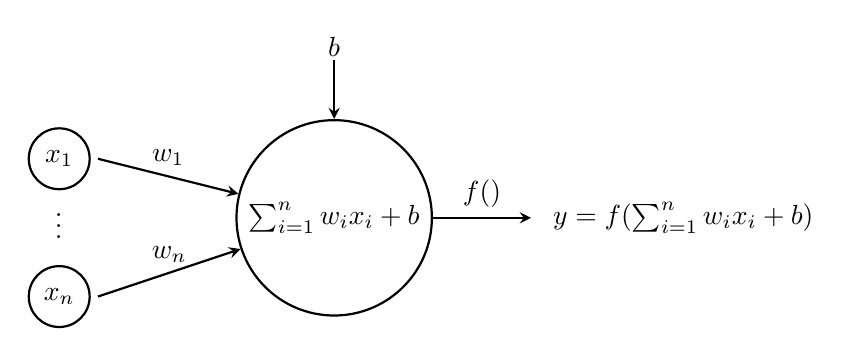
\begin{tikzpicture}
		\node[mynode](p) at (3,1){$\sum_{i=1}^{n}w_ix_i+b$};
        \node(dots) at (-0.5,1){\vdots};

        \draw[-stealth,thick] (3,3) node[yshift=5]{$b$} -- (p);
        \draw[-stealth,thick] (0,1.75) node[mynode,xshift=-14]{$x_1$} --(p) node[midway, above]{$w_1$};
        \draw[-stealth,thick] (0,0) node[mynode,xshift=-14]{$x_n$} -- (p) node[midway, above]{$w_n$};
        \draw[-stealth,thick] (p) -- (5.5,1) node[xshift=55]{$y = f(\sum_{i=1}^{n}w_ix_i+b)$} node[midway, above]{$f()$};
	\end{tikzpicture}
    \caption{An artificial neuron. Inputs are multiplied by weights and summed with a bias. The result is altered by an activation function. Figure adapted from \cite{Jurafsky.2024}.}
    \label{fig:neuron}
\end{figure}

Neural networks consist of many of these neurons connected in layers.
Typically, all neurons of a layer share an activation function, depending on its intended purpose \cite{Jurafsky.2024}.
Linear functions and sigmoids are often used in the output layer for regression and binary classification respectively.
\ac{relu} is more commonly used in hidden layers because it is computationally inexpensive.
When passing input data into the model, the values are passed through each layer consecutively, being altered by the respective weight matrices, activation functions and neuron connections they pass through.
The output(s) of the model are the result of all of the models calculations being applied to an input.

A network in which every neuron of a layer is connected to every neuron of the next is called a fully-connected network.
A simple example can be seen in figure \ref{fig:nn}.
Each connecting arrow in the figure corresponds to a unique weight value with which the value travelling along it is multiplied.
In \acp{fnn}, unlike in \acp{rnn}, data travels only in one direction, with no layer feeding back into a previous one \cite{Jurafsky.2024}.

\begin{figure}
    \centering
    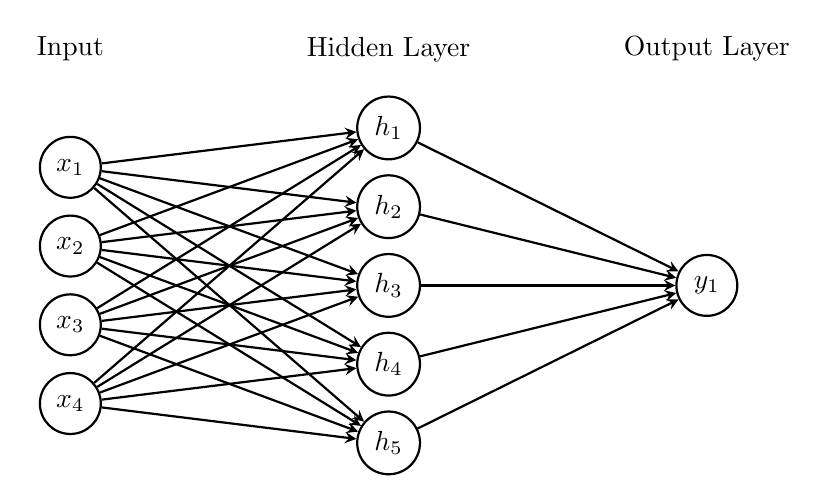
\begin{tikzpicture}[x=\textwidth/3]
    \readlist\Nnod{4,5,1}
    \foreachitem \N \in \Nnod{
        \ifnum\Ncnt=1
            \node at (\Ncnt, 3) {Input};
        \else\ifnum\Ncnt=2
            \node at (\Ncnt, 3) {Hidden Layer};
        \else
            \node at (\Ncnt, 3) {Output Layer};
        \fi\fi

        \foreach \i [evaluate={\x=\Ncnt; \y=\N/2-\i+0.5; \prev=int(\Ncnt-1);}] in {1,...,\N}{
            \ifnum\Ncnt=1
                \node[mynode] (N\Ncnt-\i) at (\x,\y) {$x_{\i}$};
            \else\ifnum\Ncnt=2
                \node[mynode] (N\Ncnt-\i) at (\x,\y) {$h_{\i}$};
            \else
                \node[mynode] (N\Ncnt-\i) at (\x,\y) {$y_{\i}$};
            \fi\fi

            \ifnum\Ncnt>1
                \foreach \j in {1,...,\Nnod[\prev]}{
                    \draw[-stealth,thick] (N\prev-\j) -- (N\Ncnt-\i);
                }
            \fi
        }
    }
    \end{tikzpicture}
    \caption{A simple fully-connected neural network consisting of an input vector of size four, a hidden layer with five neurons and an output layer with a single neuron. Figure adapted from \cite{Jurafsky.2024}.}
    \label{fig:nn}
\end{figure}

A classic example for a neural network is one that detects hand-drawn digits.
The input here would be the pixel data of the image (e. g. a $28\times28$ image would be represented by an input vector of size 784, with each number corresponding to a grayscale pixel value, as with the MNIST database\footnote{\url{https://yann.lecun.com/exdb/mnist/} (last visited on 2024-10-31)}), and the output layer would be of size ten, representing the digits zero to nine.
When inputting an image, it passes through the model layers where the weights are trained to \enquote{recognize} unique patterns to each number.
After being processed by the model, the results are passed to the output neurons, where each one returns a value between zero and one, representing a likelihood of the corresponding digit being shown in the image.
This is called a classification task, and the activation function for a multi-class classification is commonly a softmax activation function ($f(x)_i = \frac{e^{x_i}}{\sum_{j=1}^{K}e^{z_j}}$, where $K$ is the number of classes, in this case ten).

\subsubsection{Training and Optimization}
\label{sec:gradient}
In order for neural networks to learn, adapt and produce desired output, they undergo a training process.
This section will focus on supervised learning and simply refer to it as learning.
Training involves feeding a corpus of labelled data into the model and updating the model's weight matrices, including biases, according to the data.
By adjusting the weights, models control which points of data to focus on and which to neglect, and in turn learn better representations in their hidden layers.
Models are typically initialized with random weights.
During the training process, the model produces outputs -- for example, a classification label or the next word in a sequence -- based on the data that is fed in.
This output is compared to the actual, desired output with what is called a \emph{loss function}, also referred to as cost.
An example of a loss function, the mean squared loss, is shown in equation \ref{eq:msl} \cite{Jurafsky.2024}, where $y^{pred}$ is the models predicted output, and $y^{true}$ is the desired output -- the label of the data.

\begin{equation}
    L_{MS} = \frac{1}{n}\sum_{i=1}^{n}(y^{pred}_i-y^{true}_i)^2
    \label{eq:msl}
\end{equation}

The goal of model training is to \emph{minimize} the loss, meaning to calculate the predicted outputs to be as close as possible to the desired outputs -- the closer they are, the smaller the loss function gets \cite{Jurafsky.2024}.
This is done with \emph{optimizers}.
An early approach to optimization is \emph{stochastic gradient descent}, where a local minimum of the loss function is approached.
A local minimum is used because finding the global minimum in a multi-dimensional space is much more challenging due to an exponentially growing space and an increase in the number of local minima and other features that hinder the search.
Additionally, the approached minimum is rarely significantly worse than the global minimum \cite{Rumelhart.1986}.
This is done by calculating the derivative, determining the direction in which the function descends most, and adjusting the parameters to follow that trajectory.
A visualization of stochastic gradient descent is shown in figure \ref{fig:graddesc}.

This process in turn is done with \emph{backpropagation} \cite{Rumelhart.1986}.
In backpropagation, a single piece of data is sent through the model, and the loss is calculated.
The goal is to calculate a desired change in model parameters for that piece of data.
This is achieved by moving backwards through the model and calculating the necessary changes in all weight and bias parameters.
This process is done recursively, starting at the output layer and moving backwards, with each neuron calculating a desired change and passing the information back to its connections of the previous layer.
At the end of this process, a desired change for all weights and biases is recorded.
A full gradient descent step takes the backpropagation results of all points of data in the corpus and calculates the average, then applies the changes to the model.

\begin{figure}
    \centering
    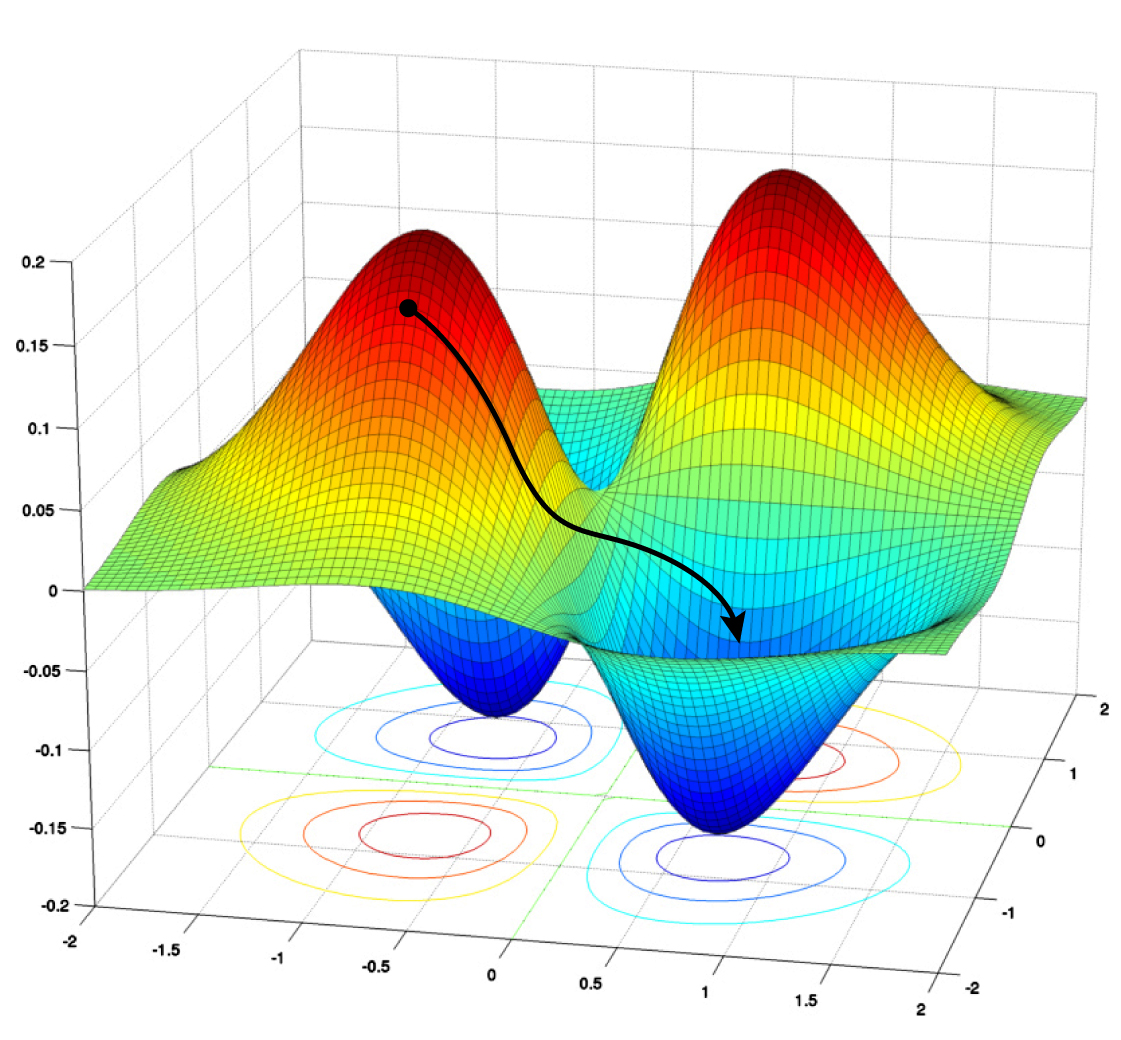
\includegraphics[width=\textwidth/2]{kapitel2/Gradient-descent.jpg}
    \caption{Gradient descent in a three-dimensional space. The graph represents the loss gradient and the black line shows a possible path that may be taken during gradient descent, which will eventually land in the minimum it is approaching\protect\footnotemark.}
    \label{fig:graddesc}
\end{figure}

\footnotetext{Image from \url{https://math.stackexchange.com/questions/406038/second-partial-derivative-test-question} (last visited on 2024-10-31) with modifications from \url{https://www.quantamagazine.org/researchers-build-ai-that-builds-ai-20220125/} (last visited on 2024-10-31)}

A more commonly used modern method is \ac{adam} \cite{Kingma.2015} or its derivatives like AdamW, which builds upon AdaGrad \cite{Duchi.2011} and RMSProp \cite{Tieleman.2012}.
Pseudocode for the \ac{adam} algorithm is shown in algorithm \ref{alg:adam}.
\ac{adam} utilizes two moment estimates, $m_t$ and $v_t$ which track the exponential moving averages of the gradient and the squared gradient respectively.
$\beta_1$ and $\beta_2$ are their respective exponential decay rates.
$m_t$ and $v_t$ are biased towards zero because they are initialized with it, which is why a bias-correction step is necessary for both.
$m_t$ and $v_t$ are both derived from $g_t$, which represents the gradient matrix of the model at step $t$, which could be once per sample, once per epoch, or once per batch.
An epoch is a full training pass of the entire dataset.
Data is sometimes grouped into so-called batches during training.
$\widehat{m}_t$ takes a role similarly to momentum.
Momentum is used to recognize if $g_t$ has a preferred direction by tracking the total average.
It can then accelerate movement in that direction, which is useful to skip over noisy gradients.
$\widehat{v}_t$ acts as variance detection and helps adjust the step size based on past gradient magnitude, allowing for large steps in a shallow gradient and small steps in steep gradients.
The weights are then updated, with $\alpha$ serving as a baseline step-size, $\widehat{m}_t$ deciding a direction and speed of the change, $\widehat{v}_t$ acting as a regulator based on the gradient and $\epsilon$ preventing division by zero. \cite{Kingma.2015}

\begin{algorithm}
    \centering
    \caption{The Adam optimizer update algorithm. $g^2_t$ is the elementwise square $g_t \odot g_t$. Kingma et al. recommend $\alpha = 0.0001$, $\beta_1 = 0.9$, $\beta_2 = 0.999$ and $\epsilon = 10^{-8}$ as default values. Algorithm taken from \cite{Kingma.2015}.}
    \begin{algorithmic}
    \Require $\alpha$: Stepsize
    \Require $\beta_1, \beta_2 \in [0,1)$: Exponential decay rates for the moment estimates
    \Require $f(\theta)$: Stochastic objective function with parameters $\theta$
    \Require $\theta_0$: Initial parameter vector

    \State $m_0 \leftarrow 0$ (Initialize 1\textsuperscript{st} moment vector)
    \State $v_0 \leftarrow 0$ (Initialize 2\textsuperscript{nd} moment vector)
    \State $t \leftarrow 0$ (Initialize timestep)

    \While{$\theta_t $ not converged}
        \State $t \leftarrow t+1$
        \State $g_t \leftarrow \nabla{\theta}f_t(\theta_{t-1})$ (Get gradients w.r.t stochastic objective at timestep $t$)
        \State $m_t \leftarrow \beta_1 \cdot m_{t-1} + (1 - \beta_1) \cdot g_t$ (Update biased first raw moment estimate)
        \State $v_t \leftarrow \beta_2 \cdot v_{t-1} + (1 - \beta_1) \cdot g^2_t$ (Update biased second raw moment estimate)
        \State $\widehat{m}_t \leftarrow m_t / (1 - \beta^t_1)$ (Compute bias-corrected first moment estimate)
        \State $\widehat{v}_t \leftarrow v_t / (1 - \beta^t_2)$ (Compute bias-corrected first moment estimate)
        \State $\theta_t \leftarrow \theta_{t-1} - \alpha \cdot \widehat{m}_t / (\sqrt{\widehat{v}_t} + \epsilon)$ (Update parameters)
    \EndWhile

    \State \Return $\theta_t$ (Resulting parameters)
    \end{algorithmic}
    \label{alg:adam}
\end{algorithm}


\subsection{Tokenization and Word Embeddings}
\label{sec:embeddings}
An important consideration in \ac{nlp} is how to feed textual data into models -- how can words be converted into a format that a model can understand?
In modern \ac{nlp}, there are two main components to this: \emph{tokenization} and \emph{word embeddings}.

Tokenization is the process of turning a text into an array of tokens using a tokenizer \cite{Jurafsky.2024,Nadkarni.2011}.
It is one of the first steps in the \ac{nlp} pipeline because models do not understand plain language string inputs, only numbers arranged into input vectors.
Tokens can be letter by letter, word for word, syllable by syllable, differentiating capital letters or not, treating special chararacters as unique tokens, among other possible groupings which are tokenizer-specific.
Tokenization is done with a vocabulary -- a mapping of known \enquote{text chunks} to their respective tokens.
Taking the example sentence \enquote{a token is a number.} and the tokenizer vocabulary \{' ' = 0, 'a' = 1, 'token' = 2, 'is' = 3, 'number' = 4, '.' = 5\}, then the resulting tokenized representation would be [1, 0, 2, 0, 3, 0, 1, 0, 4, 5].
Tokenization also includes \emph{padding} and \emph{truncation}.
Because models often have a fixed input size, any data that is inserted must be fitted to that size.
Padding adds dummy tokens to the end of the input if it is too short while truncation cuts any excess tokens if it is too long.

Embeddings are a bit more complicated.
A word embedding refers to a representation of the meaning behind a word, typically represented by a large-dimensional vector field where each dimension corresponds to some attribute of the word.
Words are often highly dependant on their context -- for example \enquote{He works at a bank}.
Which type of bank is being referred to?
Is the man is from Frankfurt, most likely a building.
If he is a fisherman, the river bank.
This is also language specific -- if the man is German, he may instead have a food truck at the park by the bench, as \enquote{Bank} can mean bench in German.
All of this information should be captured by an embedding to properly predict the most likely next word.

A well-known early embedding approach is Word2Vec, introduced by Mikolov et al. in 2013 \cite{Mikolov.2013b}.
It uses a vocabulary of around one million words and was trained on a text corpus of 6 billion words, the Google News corpus\footnote{\url{https://code.google.com/archive/p/word2vec/} (last visited on 2024-10-31)}.
The representations are trained with neural networks using stochastic gradient descent. Mikolov et al. further propose both continuous bag of words (CBOW) and Skip-gram as algorithms to predict a word from its context.
They find that in their representations, the relationships between words could be represented as algebraic operations, such as the following example: $vector("biggest") - vector("big") + vector("small")$ is roughly equivalent to $vector("smallest")$.
The same is applicable to the relationships between countries and capital cities being roughly the same vector or the famous $vector("King") - vector("Man") + vector("Woman") \approx vector("Queen")$ \cite{Mikolov.2013}.
Embeddings are often accompanied by a context size -- the number of words to look ahead and before to assess the context of each word individually.
A larger context size comes with more information, but also with more computational cost for the embedding.

In a modern system like the \ac{gpt}, the basis for ChatGPT, and the transformer architecture in general, which will be explained in further depth in section \ref{sec:transformer}, word embeddings are learned as part of the larger model alongside its other parameters \cite{Brown.2020}.
For comparison, the GPT-3 series uses word embeddings between 768 and 12.288 dimensions learned on 300 billion tokens \cite{Brown.2020} while the the Word2Vec paper examines between 50 and 1.000 dimensions for its tests \cite{Mikolov.2013b}.
Combining tokenization and embeddings is simple -- words are tokenized, the tokens are fed into the model and embeddings for the tokens are learned.
This may even allow new layers of context, especially if a word is split into multiple tokens.
The embedding for the token of \enquote{est} may contain the information that it is often a suffix and that, if at the end of a word, makes it a superlative, like the previously mentioned \enquote{biggest} and \enquote{smallest}.


\subsection{Transformers}
\label{sec:transformer}
Introduced by Google's research team in 2017 \cite{Vaswani.2017}, the transformer architecture has since become the standard for most \ac{llm} architectures.
Its defining characteristic and the paper's namesake is the self-attention mechanism, which will be explained later in this section.

A full transformer consists of one or more encoder blocks and one or more decoder blocks (introduced by \cite{Cho.2014}), as seen in figure \ref{fig:transformer}, but encoder-only (e.g. BERT \cite{Devlin.2019}) and decoder-only (e.g. GPT \cite{AlecRadfordKarthikNarasimhanTimSalimansIlyaSutskever.2018}) architectures have also become prevalent.

\begin{figure}[h]
    \centering
    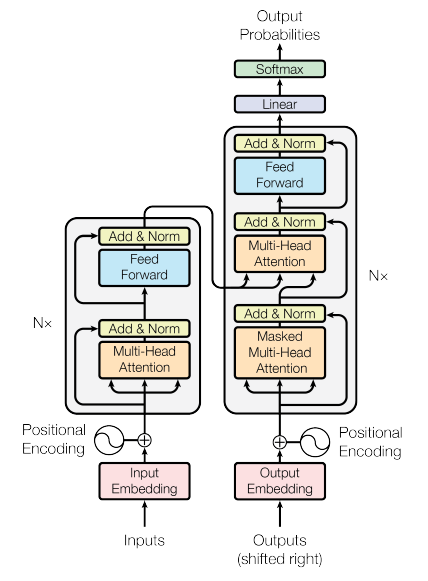
\includegraphics[width=\textwidth*2/3]{bilder/kapitel2/transformer.png}
    \caption{The full transformer architecture, consisting of embeddings, positional encoding and N encoder- and decoder blocks including attention heads and \acp{fnn}. Image taken from \cite{Vaswani.2017}.}
    \label{fig:transformer}
\end{figure}

The encoder turns an input sequence $(x_1, ..., x_n)$ into a sequence of continuous representations $z = (z_1, ..., z_n)$. The decoder generates a new output sequence $(y_1, ..., y_m)$ for a given input sequence $z$ \cite{Vaswani.2017, Cho.2014}.
More plainly, the encoder learns to create a hidden representations of a sequence of tokens and the decoder generates the most likely next token(s) to follow such a sequence.
Both blocks consist of the same components:

\paragraph{The Embedding Layer} turns the input tokens into their learned word embedding representations of size $d^{model}$ ($=512$ in the paper \cite{Vaswani.2017}).

\paragraph{The Positional Encoding} exists to add information to a token about its position within a given sequence.
These encodings have the same dimension as the embeddings, $d_{model}$, so they can be summed.
The original paper calculates the positional encoding as
\begin{equation}
    \begin{aligned}
        PE_{(pos,2i)} &= sin(pos/1000^{2i/d_{model}}) \text{ (even }i\text{)} \\
        PE_{(pos,2i+1)} &= cos(pos/1000^{2i/d_{model}}) \text{ (odd }i\text{)}
    \end{aligned}
\end{equation}
where $pos$ is the position of the token in the sequence and $i$ is the dimension of the positional encoding \cite{Vaswani.2017}.

\paragraph{The (Masked) Multi-Head Attention} is essentially a mechanism for the model to learn relationship between tokens in a sequence.
The goal of this mechanism is to calculate how closely a token is related to all other tokens.
In multi-head attention, multiple attention layers are used so that relationships can be established on different levels simultaneously, be that similar words, grammatical structure, word function, multi-token names, which noun a pronoun refers to and many more.
The original paper uses eight attention heads \cite{Vaswani.2017}.
Within the attention mechanism, a query, key and value vector are used to calculate the output with the equation
\begin{equation}
    \text{Attention}(Q,K,V)=\text{softmax}(\frac{QK^T}{\sqrt{d_k}})V
\end{equation}
where $d_k$ is the dimenion of $Q$ and $K$ \cite{Vaswani.2017}.
$Q$, $K$ and $V$ are derived from the input through learned projections.
A visualization of an attention output can be seen in figure \ref{fig:attention}.

\begin{figure}
    \centering
    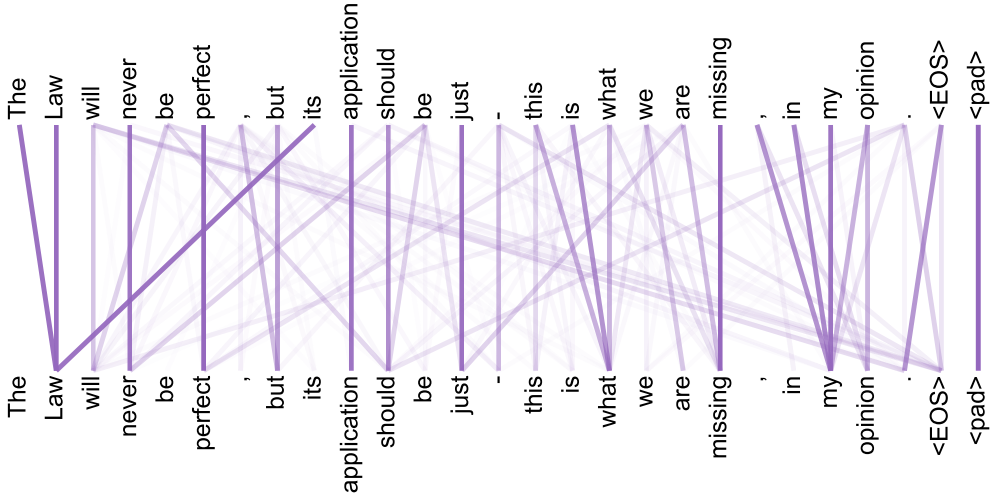
\includegraphics[width=\textwidth]{kapitel2/attention.png}
    \caption{A visualization of the output of one attention head. A darker purple means a stronger connection. For example, the word \enquote{its} strongly correlates to the word \enquote{Law}, as the former is a pronoun referring to the latter. Image taken from \cite{Vaswani.2017}.}
    \label{fig:attention}
\end{figure}

\paragraph{The Feedforward Neural Network} is, as explained in section \ref{sec:fnn}, a network of neurons grouped into layers that processes hidden representations of inputs through its layer configurations and weights learned with a training corpus.
\newline

For the original paper, the encoder layer consists of input embeddings, positional encoding, and N blocks of a multi-head attention layer followed by a feedforward layer.
These N blocks all have the exact same dimensions.
The original paper uses six heads \cite{Vaswani.2017}.
The decoder layer similarly consists of output embeddings, positional encoding, followed by N blocks of a masked multi-head attention layer, a multi-head attention layer and a feedforward block.
The outputs being shifted to the right, in combination with the masked attention, prevents the prediction for position $i$ to look ahead, instead only getting information from previous positions in the sequence.
These N blocks are also all the same, with the original paper having six \cite{Vaswani.2017}.
The outputs of the encoder layer feed into the second attention layer in the decoder block.
Finally, the outputs are run through a linear layer (a layer with a linear activation function) and a softmax layer to calculate the outputs.

The purpose of shifting the outputs right and using the masked multi-head attention layer is to limit the attention on words that come before the current token.
This is because the decoder layer calculates the probabilities for the next token in the sequence, meaning it does not have tokens following it and it can only look backwards for context.

One of the main advantages of the transformer is its high parallelizability during training, as opposed to recurrent models.
Being able to process multiple tokens simultaneously allows for much faster training, and is what enables transformers to be effectively trained on GPUs, which specialize in parallelized operations.
Because the transformer architecture has become so prevalent, when this thesis mentions \acp{lm} or \acp{llm}, it will refer to a transformer architecture unless otherwise specified.

\begin{comment}
\subsection{Code Synthesis}
\label{sec:codesynth}
(Probably don't need this section)
Code synthesis describes the generation of code syntax by a computer.

 PCFG and AST
 Code2Seq
 Latent Predictor Networks
 CodeBERT

In terms of \ac{nlp}, code is structured much differently from natural language on multiple levels.
It has a much more rigid structure that it must adhere to to work, has a much more limited vocabulary for anything other than user-given variable names (which are comparable to named entitites in regular \ac{nlp}), and it is not structured sequentially, but rather like a tree (called the \ac{ast}).
Words and punctuation can also different meanings in code and are much more strictly defined, losing much of their ambiguous context.
The word \enquote{if} would normally be followed by a pronoun and a verb in natural language, but by a condition statement in a bracket in code.
With code, much closer attention needs to be put on syntax.
If a natural \acl{lm} forgets to generate a comma, the sentence is typically still legible.
If a code synthesis model forgets a bracket, the code has an error and cannot run.
Further, code needs to be functionally correct, meaning it has to produce the desired output.
Metrics like the BLEU score break down in assessing code generation, because code that looks similar does not always behave the same, and code that does not look similar can behave identically.
\end{comment}



\subsection{Parameter-Efficient Fine-Tuning}
\label{sec:peft}

As \acp{lm} become more and more complex, fine-tuning them for specific purposes becomes a daunting task.
\acp{llm} especially have been trained on state-of-the-art hardware for months and have billions of parameters.
Fine-tuning all parameters of such a model requires an immense amount of processing power, memory and storage space.
\ac{peft} is a field of study to reduce this cost by exploring alternative ways of fine-tuning other than simple full-parameter fine-tuning.


\subsubsection{LoRA}
\label{sec:lora}

\begin{figure}
    \centering
    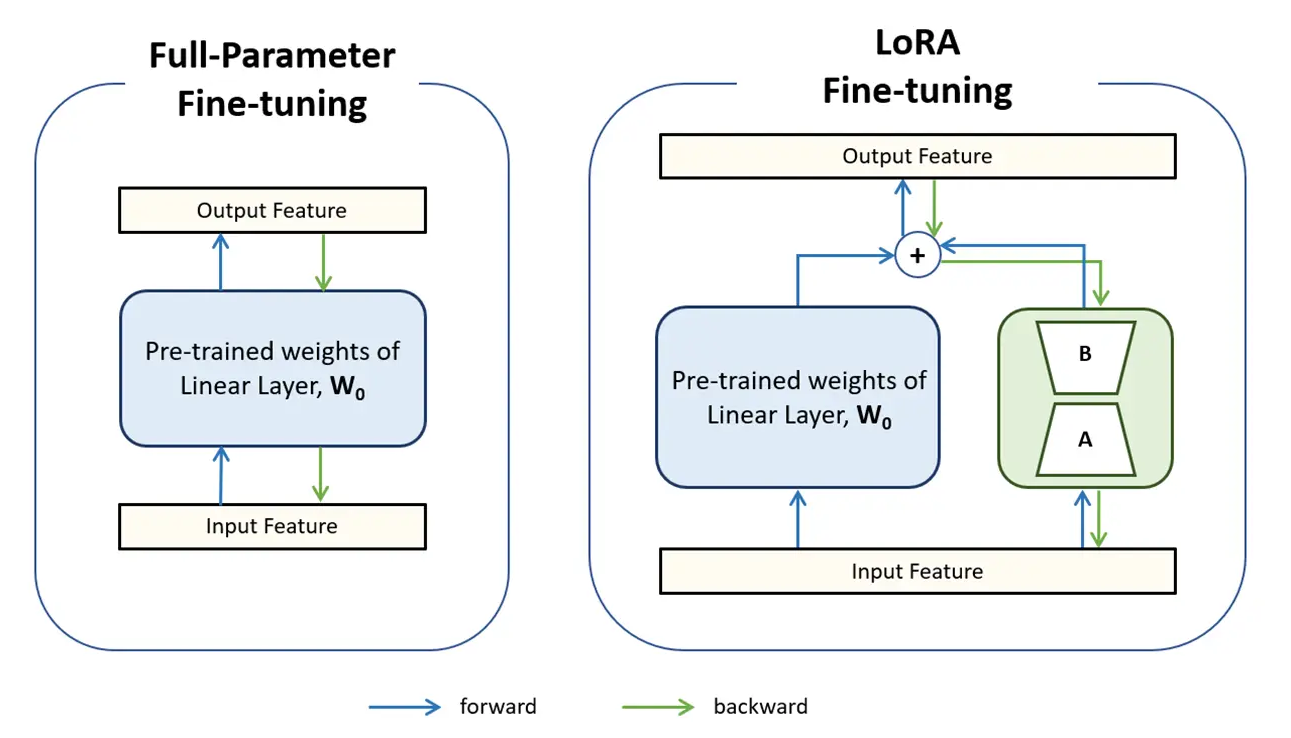
\includegraphics[width=\textwidth]{bilder/kapitel2/lora.png}
    \caption{Full-parameter fine-tuning and \ac{lora} fine-tuning. \ac{lora} adds the new matrices A and B which are trained rather than the pre-trained weights W$_0$\protect\footnotemark.}
    \label{fig:lora}
\end{figure}
\footnotetext{Image taken from \url{https://developer.habana.ai/blog/fine-tuning-llama2-70b-with-deepspeed-zero-3-and-low-rank-adaptation-lora-on-intel-gaudi2-ai-accelerator} (last visited on 2024-10-31)}

\Ac{lora} is a popular method to efficiently fine-tune \acp{lm}.
Introduced by Microsoft's Hu et al. in 2021 \cite{Hu.2022}, \ac{lora} does not directly train and alter the weights of a model.
Instead, it freezes the pre-trained weights and introduces new weights to train into the model.
This has a few advantages: Training the new weights is much less computationally intense and adding new weights lets the model keep all of its old weights intact.

It allows the training of multiple downstream tasks from a single model easily by simply saving the newly learned weights, which also saves massively on storage space the larger the model is, and it prevents \emph{catastrophic forgetting}, where weights are altered to such an extent that previously acquired knowledge is lost.
\ac{lora} configurations built onto the same model can even be swapped out at runtime, allowing a much more performant model for multiple specific tasks at reduced storage and processing costs.
\ac{lora} weights are saved as two low-ranking matrices, representing each of the dimensions of the model's weights which they aim to fine-tune \cite{Hu.2022}.
This is done because Hu et al. assert that a model's weight matrices do not need to be fully adjusted during training, and that a smaller subset of weight changes can capture the desired change equally well.
In this context, rank refers to the number of linearly independant rows or columns, and Hu et al. argue that the ranks of weight matrices are often smaller than their actual dimensions, meaning they carry superfluous information.
Given a weight matrix of a size $d \times k$ and a chosen rank $r$ between 1 and $\min(d,k)$, training with \ac{lora} would use two matrices of sizes $d \times r$ and $r \times k$, then multiply them together to get the original matrix size.
This can be expressed as

\begin{equation}
    h = W_0x + \Delta Wx = W_0x + BAx
\end{equation}

where $h$ is the fine-tuned weight matrix, $W_0 \in \mathbb{R}^{d\times k}$ is the pre-trained weight matrix and $B \in \mathbb{R}^{d\times r}, A \in \mathbb{R}^{r\times k}$ are the low-rank matrices which produce $\Delta W$ when multiplied \cite{Hu.2022}.

One might expect that finding an appropriate size for $r$ which balances performance and accuracy depends on the task.
A smaller $r$ could mean better performance as the size of the matrix is decreased, but in turn can also lead to lower accuracy as detail is lost if the chosen rank is lower than the \enquote{optimal rank} for the respective weights.
However, as the original paper finds, very small ranks, even a rank of one, are sufficient for fine-tuning in many cases, and applying \ac{lora} to more weight matrices with a lower rank is preferable to applying it to fewer matrices with a larger one \cite{Hu.2022}.

\subsubsection{QLoRA}
\label{sec:qlora}
Dettmers et al. introduced \ac{qlora} in 2023 \cite{Dettmers.2023}, building upon the low-rank approach introduced with \ac{lora}.
Quantization refers to the act of transforming a piece of information or data into a representation that holds less information.
In the case of computers, this means transforming higher-bit representations into lower-bit representation.
\ac{qlora} contains three primary contributions: NF4, double quantization and paged optimizers.
NF4 refers to 4-bit NormalFloat, a newly introduced datatype that builds on quantile quantization.
It works as follows:
It estimates $2^l+1$ quantiles from the input to create a $k$-bit quantile quantization data type, normalizes them to $[-1,1]$.
It also quantizes an input weight tensor, also normalizing it to $[-1,1]$ through absolute maximum rescaling and with the help of quantization constants.
Dettmers. et al. posit that weight tensors often follow a zero-centered normal distribution with a standard deviation $\sigma$, which allows this normalization into a fixed distribution.
Quantiles are estimated according to

\begin{equation}
    q_i = \frac{1}{2} \left( Q_{\mathrm{x}} \left( \frac{i}{2^k+1} \right) + Q_{\mathrm{x}} \left( \frac{i+1}{2^k+1} \right) \right)
\end{equation}

where $Q_{\mathrm{x}}(\cdot)$ is the quantile function of the standard normal distribution $N(0,1)$ \cite{Dettmers.2023}.
Once the input and data types are normalized, the inputs can be mapped to the closest quantized representation.
In order to represent zero, two symmetric quantile sets are estimated, one for a positive range (of size $2^{k-1}+1$) and one for a negative range (of size $2^{k-1}$).
One of the zeroes is discarded and the two sets are combined into an asymmetric set with a single zero at its center.
The resulting information-theoretically optimal data type is called $k$-bit NormalFloat (NF$k$), with \ac{qlora} using $k=4$ \cite{Dettmers.2023}.

Double quantization takes the quantization constants $c_2$\textsuperscript{FP32} of the first quantization and quantizes them to save even more memory.
It transforms them into $c_2$\textsuperscript{FP8} with its own set of quantization constants $c_1$\textsuperscript{FP32}.
The superset text refers to the bit size or data type of the respective value, in this case 8-bit or 32-bit floating point.
Dettmers et al. calculate a reduction of 0.5 bits to 0.127 bits per parameter on average for a blocksize of 64 and 32-bit floating point constants \cite{Dettmers.2023}.
Paged optimizers utilize NVIDIAs unified memory to offload processing from the GPU to the CPU when the GPU runs out of memory.
Combining everything, Dettmers et al. define the output for a single linear layer of a quantized base model with one \ac{lora} adapter using \ac{qlora} as

\begin{equation}
    \mathbf{Y}^{\text{BF16}} = \mathbf{X}^{\text{BF16}} \text{doubleDequant} (c_1^{\text{FP32}},c_2^{\text{k-bit}},\textbf{W}^{\text{NF4}}) + \mathbf{X}^{\text{BF16}} \mathbf{L}_1^{\text{BF16}} \mathbf{L}_2^{\text{BF16}}
\end{equation}
with
\begin{equation}
    \text{doubleDequant} (c_1^{\text{FP32}},c_2^{\text{k-bit}},\textbf{W}^{\text{k-bit}}) = \text{dequant}(\text{dequant}(c_1^{\text{FP32}},c_2^{\text{k-bit}}), \textbf{W}^{\text{4-bit}}) = \textbf{W}^{\text{BF16}}
\end{equation}
where $\mathbf{X}$ is the input, $\mathbf{W}$ are the quantized weights, $\mathbf{Y}$ is the output, $c_1$ and $c_2$ are the quantization constants and $L_1$ and $L_2$ are equivalent to the \ac{lora} matrices $A$ and $B$ explained in section \ref{sec:lora} \cite{Dettmers.2023}.

During evaluation, they establish that 4-bit \ac{qlora} matches 16-bit full finetuning in performance on benchmarks like GLUE \cite{Wang.2018} and T$k$-Instruct \cite{Wang.2022}.
They note that \ac{qlora} reduces the average memory requirements of finetuning a 65 B parameter model from over 780 GB GPU memory to under 48 GB without affecting the runtime or model performance when compared to full 16-bit finetuning.
They also finetune the Guanaco 65 B model on OASST1 using \ac{qlora}, producing the best open-source chatbot of its time, comparable in performance to ChatGPT on the Vicuna benchmark \cite{Chiang.2023}.
Their thesis concludes that \ac{qlora} makes the creation of performant models much more accessible because of the reduced cost for training models \cite{Dettmers.2023}.


\section{Evaluation Metrics}
\label{sec:metrics}

Because the development of code synthesis \acp{lm} has become increasingly popular, many metrics and frameworks for testing their coding ability have been developed.
This section will introduce some of these metrics and frameworks, which will be used to judge the coding ability of the TinyFuncCoder models introduced by this thesis.
Many of the presented metrics are part of the Bigcode Evaluation Harness \cite{BenAllal.2022}, a collection of metrics for assessing code synthesis ability of \acp{lm}.
The metrics of the BigCode Evaluation Harness that did not get their own sections were not considered for the following reasons:
\begin{itemize}
    \item InstructHumanEval\footnote{\url{https://huggingface.co/datasets/codeparrot/instructhumaneval} (last visited on 2024-10-31)} reformats the HumanEval prompt and is incompatible with the prompt template for TinyFuncCoder.
    \item APPS \cite{Hendrycks.2021} consists of 10.000 Python problems. Python is overrepresented in the evaluation metrics, as discussed in chapter \ref{chap:discussion}, and evaluating on 10.000 problems is not feasible within the time constraints of the thesis.
    \item Recode \cite{Wang.2022} perturbs HumanEval problems, effectively just increasing the amount of problems close to identical to HumanEval the model has to solve.
    \item PAL \cite{Gao.2023} is not compatible with TinyFuncCoder's prompt template.
    \item CodeXGLUE \cite{Lu.2021} is a code to text task, which TinyFuncCoder is not trained for.
    \item CoNaLa (Python) \cite{Yin.2018} and Concode (Java) \cite{Iyer.2018} use BLEU, which is deemed an unsuitable metric for code synthesis evaluation \cite{Chen.2021,Luo.2024}.
    \item Java complexity prediction \cite{Jeon.2023}, Java code equivalence prediction \cite{Svajlenko.2014,Wang.2020} and C code defect prediction \cite{Zhou.2019} are downstream classification tasks, which TinyFuncCoder is not trained for.
    \item SantaCoder-FIM \cite{Allal.2023} is an infilling task, which TinyFuncCoder is not trained for.
    \item Mercury \cite{Du.2024} evaluates code efficiency, which TinyFuncCoder is not capable enough to benefit from analyzing.
\end{itemize}

\subsection{HumanEval}
\label{sec:humaneval}
In their 2021 paper, Chen et al. introduce the Codex \ac{llm} and -- more importantly for this thesis -- the HumanEval evaluation framework \cite{Chen.2021}.
The HumanEval framework is a set of programming challenges with associated unit tests.
It judges the coding ability of \acp{lm} by prompting them with a challenge and then seeing if the resulting code passes its unit tests.
This method of checking functional correctness differs from previously used \ac{nlp} metrics like the BLEU score \cite{Papineni.2001}, which matches or fuzzy matches the output to an existing, expected result.
Because the BLEU score has been found as inefficient \cite{Chen.2021,Luo.2024}, Chen et al. use the pass@$k$ metric \cite{Kulal.2019}.
They deviate from the original definition where $k$ samples are generated and pass@$k$ is defined by $\frac{c}{k}$, where $c$ is the number of samples that pass all tests.
Instead, they give a mathematically less biased definition that reduces the otherwise high variance:
\begin{equation}
    \text{pass@}k := \underset{\text{Problems}}{\mathbb{E}} \left[ 1 - \frac{ \left( \begin{array}{c} n-c \\ k \end{array} \right) }{ \left( \begin{array}{c} n \\ k \end{array} \right) } \right]
    \label{eq:passk}
\end{equation}
where $n \geq k$ samples are generated and $c \leq n$ correct samples are produced \cite{Chen.2021}.
Commonly, either pass@1, pass@10 or pass@100 are used for evaluation.
Pass@$k$ has become the metric of choice for evaluating code synthesis ability on most benchmarks.

HumanEval consists of 164 hand-written challenges with an average of 7.7 tests per problem.
The problems include a function signature, docstring, the tests and a body.
They are written exclusively in Python, meaning it can only evaluate how good the Python code a model can synthesise is \cite{Chen.2021}.
As the paper focuses mainly on Codex, not much detail is given as to how the questions were written and decided on. % page 25
It is simply stated that they assess \enquote{language comprehension, reasoning, algorithms, and simple mathematics} \cite{Chen.2021}.
The appendix adds some elaboration and goes into detail about the attributes that were focused on when creating the dataset, but still does not give a proper explanation for its creation.

When evaluating on HumanEval, Chen et al. find that the temperature used for generation should be chosen in relation to $k$ when evaluating on the pass@$k$ metric.
The temperature regulates the amount of randomness in the generation, with a temperature of zero always giving the same result, and a temperature of one varying wildly in output.
They specify that $k$=1 should have a temperature of around 0.2 when generating and $k$=100 a temperature of around 0.8.
On their largest model with $10^{10}$ parameters, they achieve a pass@1 of around 30\% and a pass@100 of around 70\% using the previously given temperatures.

\subsection{MBPP}
\label{sec:mbpp}
\ac{mbpp} was introduced by Odena et al. of Google Research \cite{Odena.2021} alongside MathQA-Python.
It consists of 974 programming tasks intended to be solvable by entry-level programmers.
They are given as a natural language prompt with three example calls to the function with an expected result in the form of assertions the function should pass.
Similarly to HumanEval, these tasks are all given exclusively in Python.

When evaluating code synthesis ability, Odena et al. note that larger models perform better, with the largest at 137 B parameters synthesising solutions for 59.6\% of problems with few-shot learning.
They further note that fine-tuning on their set of only 374 problems improves performance by around ten percent across all models.

To create the dataset, crowdworkers with knowledge of Python were asked to write basic Python problems, a corresponding solution, and three test cases for the given function.
A hand-filtered subset of this dataset was also created.
This resulted in a dataset of 476 problems for which the authors ensure a standard Python signature, an unambiguous description and accurate test cases.
Both the full set and the edited set were used in their testing.


\subsection{EvalPlus}
\label{sec:evalplus}

\begin{figure}
    \centering
    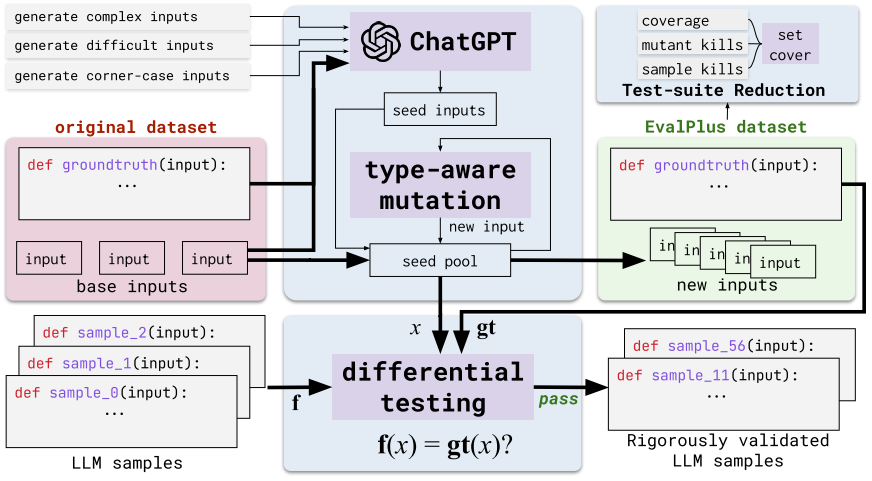
\includegraphics[width=\textwidth]{bilder/kapitel2/evalplus.png}
    \caption{Generation of new test cases using the EvalPlus framework. Image taken from \cite{Liu.2024}.}
    \label{fig:evalplus}
\end{figure}

The EvalPlus framework, introduced by Liu et al. \cite{Liu.2024}, aims to improve upon other code synthesis assessment metrics by expanding their test suites with the help of \acp{llm}.
Their paper mainly showcases this framework when applied to HumanEval, creating HumanEval+, but they have since also created MBPP+ with it.
As it only expands the test coverage, the problems are identical to the base versions but the generated results are checked more thoroughly, and by extension so is model performance on the pass@$k$ metric.

Their main points of criticism of coding metrics are that problems are given with imprecise descriptions and with an average of less than ten tests per problem.
They argue that imprecise descriptions fail to fully clarify the expected behaviours of the generated code and that a lack of proper testing leads to many false positives because edge cases are not properly covered.

The EvalPlus framework generates new test cases as follows:
First, it takes the original ground-truth implementations and one of its three test cases as an input. Together with a prompt (one of \enquote{generate [complex|difficult|corner-case] inputs}), ChatGPT is queried to generate seed inputs, only filtering out results which do not adhere to the format expected by the ground-truth implementation.

Next, type-aware input mutation \cite{Winterer.2020} is performed on the seed inputs. This means altering the provided test cases by altering the given inputs in some way. Inputs are altered differently depending on their data type, hence type-aware. The applied mutations are listed in table \ref{tab:mutation}.
%\renewcommand{\arraystretch}{1.2}

\begin{table}
    \centering
    \small
    \caption{Mutations used by the EvalPlus framework to alter inputs. \texttt{Mutate} refers to a recursive function to alter an inner type (for example, the int mutation can be applied to a random subset of a list of ints). Table taken from \cite{Liu.2024}.}
    \begin{tabular}{ll|ll}
        \hline
        Type & Mutation & Type & Mutation\\
        \hline
        \texttt{int} | \texttt{float} & Returns $x\pm1$ &
        \texttt{List} & $\left\{\begin{tabular}{@{\ }l@{}}
            Remove/repeat a random item $x[i]$ \\ Insert/replace $x[i]$ with \texttt{Mutate($x[i]$)}\end{tabular}\right.$ \\
        \texttt{bool} & Returns a random boolean &
        \texttt{Tuple} & Returns \texttt{Tuple(Mutate(List($x$)))} \\
        \texttt{NoneType} & Returns \texttt{None} &
        \texttt{Set} & Returns \texttt{Set(Mutate(List($x$)))}\\
        \texttt{str} & $\left\{\begin{tabular}{@{\ }l@{}}
            Remove a sub-string $s$ \\ Repeat a sub-string $s$  \\ Replace $s$ with \texttt{Mutate}($s$)\end{tabular}\right.$ &
    \texttt{Dict} & $\left\{\begin{tabular}{@{\ }l@{}}
            Remove a key-value pair $k\rightarrow v$ \\ Update $k\rightarrow v$ to $k\rightarrow$ \texttt{Mutate($v$)}  \\ Insert \texttt{Mutate($k$)$\rightarrow$Mutate($v$)}
    \end{tabular}\right.$ \\
        \hline
    \end{tabular}
    \label{tab:mutation}
\end{table}

Finally, a smaller subset called HumanEval+-Mini is created by reducing the HumanEval+ set by a factor of 47, focusing on keeping a similar branch coverage and pruning tests through mutation testing and \ac{llm} sample killings.
A full overview of this process is shown in figure \ref{fig:evalplus}.
To ensure that their tests work, they follow the principle of design by contract \cite{Meyer.1992}, which they implement through assert statements to ensure well-formed inputs.

Liu et al. also tested HumanEval+ with over 26 \acp{llm} and various temperature settings.
They find that performance on the pass@$k$ metric (\ref{eq:passk}) sank across the board in all tests, with drops of 19.3\%, 24.9\% and 28.9\% for $k$ = 1, 10 and 100 respectively.
HumanEval+-Mini achieves similar results, with the drop in performance being slightly less than with the full suite.
They also found that around 11\% of the original ground-truth implementations were incorrect and reimplemented them.

\subsection{MultiPL-E}
\label{sec:multiple}
MultiPL-E, introduced by Cassano et al. \cite{Cassano.2023}, extends HumanEval and \ac{mbpp} to 18 programming languages, the first massively multilingual code generation benchmark according to the paper.
It does this by writing a compiler for each language that translates the function head and tests from Python to the language.
Each compiler is around 200 lines of code.
Python-specific description vocabulary is also altered manually, and typing discrepancies between languages are taken into consideration, such as translating Python tuples and lists into JavaScript arrays.
Having a compiler for each language also makes the benchmark easily extendible.

When testing MultiPL-E with Codex \cite{Chen.2021}, CodeGen \cite{Nijkamp.2022} and InCoder \cite{Fried.2023}, Cassano et al. replicate the findings on Python performance from these three models and achieve surprisingly good results on most languages, even those that were not included in the original training sets for the models.
They also find that performance on JavaScript and TypeScript problems is similarly high to, and sometimes exceeds, performance on Python problems.

\subsection{HumanEvalPack}
\label{sec:octopack}
Similarly to MultiPL-E, the HumanEvalPack, introduced by Muennighoff et al. \cite{Muennighoff.2024}, aims to expand HumanEval by multiple languages.
Rather than the 18 of MultiPL-E, HumanEvalPack extends to six languages and does not include MBPP.
Like most other problem packs, it evaluates on the pass@$k$ metric and features three sets of problems: HumanEvalFix for repairing buggy code, HumanEvalExplain for explaining given code and then generating a solution this explanation, and HumanEvalSynthesize for generating new code (corresponding to the original HumanEval).
For HumanEvalFix, a bug was manually added to each of the 164 HumanEval problems for each of the six languages for the model to solve.
This gives an equivalent size of $164\cdot6$ for all three sections, or a total of 2952.
All the new content of the HumanEvalPack is created by humans, unlike MultiPL-E, which compiles problems to new languages or EvalPlus, which generates new problems through mutation.


\subsection{DS-1000}
\label{sec:ds1000}
DS-1000 is a set of 1000 data science problems to evluate code synthesis performance.
It was introduced by Lai et al. \cite{Lai.2023}.
The problems are all given in Python, like MBPP and HumanEval, and span seven Python libraries: NumPy\footnote{\url{https://numpy.org/} (last visited on 2024-10-31)}, Pandas\footnote{\url{https://pandas.pydata.org/} (last visited on 2024-10-31)}, TensorFlow\footnote{\url{https://www.tensorflow.org/} (last visited on 2024-10-31)}, PyTorch\footnote{\url{https://pytorch.org/} (last visited on 2024-10-31)},
SciPy\footnote{\url{https://scipy.org/} (last visited on 2024-10-31)}, Scikit-learn\footnote{\url{https://scikit-learn.org/stable/} (last visited on 2024-10-31)} and Matplotlib\footnote{\url{https://matplotlib.org/} (last visited on 2024-10-31)}.
The problems in DS-1000 are collected from StackOverflow.
They were then manually curated and altered to adhere to three principles:
First, problems that are diverse in form and content, rather than highly structured, were chosen to better reflect real-world applications.
Second, five of the paper's authors adapted these natural problems by writing new code, adapting them to be more unambiguous, executable and testable, and writing tests for them.
Third, to prevent models from simply memorizing solutions from StackOverflow, they took active measures to perturb each problem.
Perturbations include paraphrasing a problem and altering semantic components \cite{Lai.2023}.
DS-1000 presents the problems in an infilling context, though many models lack this feature and can only generate left-to-right, meaning generating new tokens at the end of a sequence, rather than in the middle.
To address this, they offer a prompt to reformat the questions for left-to-right models, while acknowledging that these will still lack behind models with infilling capabilities.

Models from three families were also tested on DS-1000, with the best results coming from codex-davinci-002 (from the Codex family which was introduced alongside HumanEval \cite{Chen.2021}) at a pass@1 of 43.3\% when infilling and 39.2\% when generating left-to-right.
This leaves much room for improvement, with even the current best model, Claude 3.5 Sonnet, achieving a pass@1 of 54.3\%.
Many models have improved on codex-002 however, with it being in 29th place on the DS-1000 leaderboard\footnote{\url{https://ds1000-code-gen.github.io/model_DS1000.html} (last visited on 2024-10-31)}.


\subsection{LeetCode Contest Benchmark}
\label{sec:leetcode}
LeetCode\footnote{\url{https://leetcode.com/} (last visited on 2024-10-31)} is a website offering coding challenges for programmers to test and expand their skills in various categories and languages, with some of these being notoriously difficult.
It also offers code interview crash courses.
In their paper introducing DeepSeek-Coder, Guo et al. \cite{Guo.2024} also introduce the LeetCode Contest Benchmark\footnote{\url{https://github.com/deepseek-ai/DeepSeek-Coder/tree/main/Evaluation/LeetCode} (last visited on 2024-10-31)}, a collection of 180 LeetCode Contest challenges from July 2023 to January 2024, with 100 test cases per challenge.
These problems are formatted in the same way as HumanEval problems and are also only given in Python.
They gather these challenges to further evaluate DeepSeek-Coder, choosing 180 challenges that at the time of the papers release would not have appeared in their training data.
This is the only benchmark mentioned that is not featured in Bigcode's evaluation harness.

When evaluating model performance, their 6.7 B parameter model achieves a pass@1 of 19.4\% with the 33 B version achieving 27.8\%.
They further note that \ac{cot} prompting improved model performance on this benchmark, especially with more challenging problems.

\section{The Stack Dataset}
\label{sec:thestack}

Bigcode's The Stack \cite{Kocetkov.2023} is a 6.4 TB dataset encompassing permissively licensed GitHub files in 358 programming languages (the paper lists 3.1 TB with 30 languages, but the set has since expanded).
It is part of the BigCode project\footnote{\url{https://www.bigcode-project.org/} (last visited on 2024-10-31)}, a scientific collaboration to openly and transparently develop and share results in the code synthesis field.

There are various versions of The Stack\footnote{\url{https://huggingface.co/datasets/bigcode/the-stack} (last visited on 2024-10-31)}, including The Stack v2\footnote{\url{https://huggingface.co/datasets/bigcode/the-stack-v2} (last visited on 2024-10-31)} at 67.5 TB, as well as near-deduplicated versions\footnote{\url{https://huggingface.co/datasets/bigcode/the-stack-dedup}}\footnote{\url{https://huggingface.co/datasets/bigcode/the-stack-v2-dedup} (last visited on 2024-10-31)} of both.
Further, there is The Stack smol\footnote{\url{https://huggingface.co/datasets/bigcode/the-stack-smol} (last visited on 2024-10-31)}, a scaled-down version with 10.000 randomly sampled files per language, totalling 2.6 GB of data.

This thesis will work with the original The Stack's 3 TB deduplicated version.
The Stack v2 currently does not include the code as a string, for which the original has the \enquote{content} column, and the deduplicated version is recommended for training by the authors.
The Stack smol was used in preparation of the codebase for this thesis before The Stack was used for dataset creation.

The Stack dataset has the following data fields, as explained on huggingface:
\begin{itemize}
    \item \texttt{content} (\texttt{string}): the content of the file.
    \item \texttt{size} (\texttt{integer}): size of the uncompressed file.
    \item \texttt{lang} (\texttt{string}): the programming language.
    \item \texttt{ext} (\texttt{string}): file extension
    \item \texttt{avg\_line\_length} (\texttt{float}): the average line-length of the file.
    \item \texttt{max\_line\_length} (\texttt{integer}): the maximum line-length of the file.
    \item \texttt{alphanum\_fraction} (\texttt{float}): the fraction of characters in the file that are alphabetical or numerical characters.
    \item \texttt{hexsha} (\texttt{string}): unique git hash of file
    \item \texttt{max\_\{stars|forks|issues\}\_repo\_path} (\texttt{string}): path to file in repo containing this file with maximum number of \{stars|forks|issues\}
    \item \texttt{max\_\{stars|forks|issues\}\_repo\_name} (\texttt{string}): name of repo containing this file with maximum number of \{stars|forks|issues\}
    \item \texttt{max\_\{stars|forks|issues\}\_repo\_head\_hexsha} (\texttt{string}): hexsha of repository head
    \item \texttt{max\_\{stars|forks|issues\}\_repo\_licenses} (\texttt{string}): licenses in repository
    \item \texttt{max\_\{stars|forks|issues\}\_count} (\texttt{integer}): number of \{stars|forks|issues\} in repository
    \item \texttt{max\_\{stars|forks|issues\}\_repo\_\{stars|forks|issues\}\_min\_datetime} \\(\texttt{string}): first timestamp of a \{stars|forks|issues\} event
    \item \texttt{max\_\{stars|forks|issues\}\_repo\_\{stars|forks|issues\}\_max\_datetime} \\(\texttt{string}): last timestamp of a \{stars|forks|issues\} event
\end{itemize}
Of these, \texttt{content}, \texttt{lang}, \texttt{hexsha} and \texttt{max\_stars\_count} are used in this thesis, as further explained in section \ref{sec:data}.

The stack was created by first gathering a list of 220.92 M unique, active GitHub repository names from GHArchive\footnote{\url{http://www.gharchive.org/} (last visited on 2024-10-31)}, of which 137.36 M were succesfully downloaded.
Of the files contained in the repositories, binary files and files exceeding 1 MB are removed, resulting in 5.28 B files in total.
Next, the files were checked for their license using GHArchive and the go-license-detector\footnote{\url{https://github.com/src-d/go-license-detector} (last visited on 2024-10-31)} and only files with a permissive license were kept.
These files are then deduplicated \cite{He.2010} and near-deduplicated, removing all files that are copies or mostly overlapping, keeping a total remained of 3.1 TB of data \cite{Kocetkov.2023}.
Note that these numbers are from the time of the paper's release and the dataset has since grown.

A further filtered Python subset of The Stack was also used to train a 350 M parameter decoder-only transformer from scratch, achieving middling results with a pass@1 of 13.94 and pass@100 of 37.00 on HumanEval, and pass@1 of 15.94 and pass@100 of 54.69 on MBPP, but outperforming the similarly-sized Codex \cite{Chen.2021} and CodeGen \cite{Nijkamp.2022} \cite{Kocetkov.2023}.
How The Stack is filtered into TinyFuncData in this thesis is explained in section \ref{sec:data}.


\section{Base Models}
\label{sec:basemodels}

This section will introduce the base models that were considered for fine-tuning to create the TinyFuncCoder series.
It will explore possible options and present their up- and downsides.

\subsection{TinyLlama}
\label{sec:tinyllama}

TinyLlama\footnote{\url{https://huggingface.co/TinyLlama/TinyLlama-1.1B-Chat-v1.0} (last visited on 2024-10-31)} is a 1.1 B parameter model pre-trained on both natural language through SlimPajama \cite{Soboleva.2023} and code through Starcoderdata \cite{Li.2023b} at a ratio of about 7:3.
It was developed by Zhang et al. \cite{Zhang.2024} as a response to \ac{nlp} research focusing on increasingly larger models, aiming to show that small models can also achieve solid performance.
To achieve this, they pre-train a decoder-only transformer architecture on almost 3 T tokens -- 950 B tokens for three epochs.
The idea behind TinyLlama -- to squeeze as much performance as possible out of a small model -- makes it an obvious pick as a base model for TinyFuncCoder.
What makes it even more suited as a choice is that it is entirely open-source and advertises itself as an improvement in accessibility for \ac{lm} research and usage.

As stated in section \ref{sec:motivation}, being pretrained on Starcoderdata could be beneficial, but it could also be detrimental.
Having previous training on code could strengthen the new information injected during training, acting as a solid baseline to expand upon.
Because TinyFuncCoder aims to be very restrictive in its possible outputs however, prior code knowledge could also lead to unexpected behaviour and undesired answer formats.
When testing on HumanEval, TinyLlama achieves a score of 9.15.
It is unspecified for which metric, but a reasonable assumption is pass@1, placing it between Codex-85M and Codex-300M \cite{Chen.2021}.
The best Codex model, Codex-12B, achieves a pass@1 of 28.81\%.

During the writing of this thesis, a newer version of TinyLlama, TinyLlama v1.1\footnote{\url{https://huggingface.co/TinyLlama/TinyLlama_v1.1} (last visited on 2024-10-31)} was released.
It is split into three models -- a base version trained and fine-tuned only on SlimPajama, a math and code version fine-tuned on Starcoderdata and Proofpile\footnote{\url{https://huggingface.co/datasets/hoskinson-center/proof-pile} (last visited on 2024-10-31)}, and a Chinese version fine-tuned on Skypile \cite{Wei.2023}.


\subsection{Phi}
\label{sec:phi}
The Phi models\footnote{\url{https://huggingface.co/collections/microsoft/phi-3-6626e15e9585a200d2d761e3} (last visited on 2024-10-31)} (Phi-1, Phi-1.5, Phi-2 and Phi-3) were developed by Microsoft as a suite of performant, small \acp{lm} of between 1.3 B and 3.8 B parameters \cite{Gunasekar.2023,Li.2023,MojanJavaheripi.2023,Abdin.2024}.
Phi-1 is mostly trained for Python coding, achieving a pass@1 of 50.4\% on HumanEval and 55.5\% on MBPP \cite{Gunasekar.2023}.
Phi-1.5 expands Phi-1 to commonsense reasoning in natural language \cite{Li.2023}, with Phi-2 and Phi-3-mini mainly focused on scaling up the model to improve its capabilities, increasing the size to 2.7 B parameters and then to 3.8 B parameters.
Microsoft claim that Phi-3-mini can run on a smartphone, occupying only 1.8 GB of memory, while still being comparable to models like Mixtral with 8x7 B parameters.
Phi-3-mini also reaches a pass@1 of 58.5 on HumanEval and 70 on MBPP \cite{Abdin.2024}.
For TinyFuncCoder, Phi-1 and 1.5 are realistically usable as baselines, but 2 and 3 are too big for fine-tuning with limited hardware.
a Phi-1-small model also exists, which retains 45\% performance on HumanEval with only 350 M parameters, but this version is not open source.

\subsection{Gemma}
\label{sec:gemma}

The Gemma series\footnote{\url{https://huggingface.co/collections/google/gemma-2-release-667d6600fd5220e7b967f315} (last visited on 2024-10-31)} is Googles open-source implementation of small decoder-only \acp{lm}, built from the same technology as Gemini \cite{GemmaTeam.2024}.
Google, similarly to Microsoft and TinyLlama, state their intent to make \acp{lm} more accessible.
The Gemma family encompasses a collection of models ranging from 2 B parameters to 27 B.
They are trained on a diverse dataset including web content, code and math, and the models were trained with between 2 T and 13 T tokens.
On HumanEval, the 2 B model achieves a pass@1 of 22 and on MBPP 29.2.
CodeGemma\footnote{\url{https://huggingface.co/collections/google/codegemma-release-66152ac7b683e2667abdee11} (last visited on 2024-10-31)}, an offshoot specifically trained for coding, improves on this, with the 2 B variant achieving 31 on HumanEval and 43.6 on MBPP \cite{CodeGemmaTeam.2024}.
The base version of Gemma being trained on a wide variety of data is promising as a base model for TinyFuncCoder, but 2 B parameters could already be too big for fine-tuning.

\begin{comment}
    \subsection{Qwen X}
    \label{sec:qwen}
    Developed by the Alibaba Group, Qwen is a series of models ranging from 0.5 B parameters to 72 B parameters \cite{Team.2024,Bai.28.09.2023,Yang.2024}.
    All of these models are trained on an 18 T token dataset, including 5.5 T tokens of code-related data.
\end{comment}
\chapter{Related Work}
\label{chap:related}

This chapter will showcase similar or relevant research to this thesis.
Section \ref{sec:starcoder} will show Starcoderdata, a dataset used by various code synthesis models for training or further data extraction.
Section \ref{sec:synthmodels} will show other models trained for code synthesis and their approach to dataset creation, architecture and training.

\section{Starcoderdata}
\label{sec:starcoder}
The Starcoderdata dataset\footnote{\url{https://huggingface.co/datasets/bigcode/Starcoderdata} (last visited on 2024-10-31)} is the dataset used for training the StarCoder code synthesis model.
Both were introduced by Li et al. \cite{Li.2023} as part of the BigCode umbrella, like The Stack dataset.
In fact, Starcoderdata is derived from The Stack (v1.2), which was introduced in section \ref{sec:thestack}.
To create Starcoderdata, Li et al. first chose all languages with over 500 MB of data, as well as the top 50 popular languages on GitHub as of December 2022\footnote{\url{https://web.archive.org/web/20221229040526/https://www.tiobe.com/tiobe-index/} (last visited on 2024-10-31)}, excluding unsupported and configuration languages, and including dialects of selected languages.
They then apply many -- often language- or language group-specific -- filters to their data, such as excluding files that begin with an XML header or files that have less than 25\% alphabetic characters.
This first pass gives them 815 GB of data, or close to 306 million files of code.

Next, they individually process all Jupyter Notebooks, GitHub issues and Git commits, and then deduplicate the dataset.
To deduplicate, they follow Allal et al.'s pipeline \cite{Allal.2023}.
They apply this pipeline to everything except for GitHub issues and Git commits.
Finally, they re-weigh JSON and YAML to 1 GB and CSS to 3 GB, arguing that all other languages are properly represented and balanced.
This results in the Starcoderdata dataset, with 207 M rows of data.


\section{Code Synthesis Models}
\label{sec:synthmodels}

This section will showcase code synthesis models introduced in other works, exploring how and on what data they have been trained and how well they perform.
This list is by no means exhaustive, as training code models is very popular at the moment (CodeLlama \cite{Roziere.2023}, CodeQwen \cite{Bai.2023}, WaveCoder \cite{Yu.2024} and many more are listed on the EvalPlus leaderboard\footnote{\url{https://evalplus.github.io/leaderboard.html} (last visited on 2024-10-31)} alone).


\subsection{WizardCoder}
\label{sec:wizardcoder}
WizardCoder, developed by Luo et al. \cite{Luo.2024}, is a code synthesis model trained with WizardLM's Evol-Instruct approach \cite{Xu.2024}.
It was fine-tuned from StarCoder, the model originally trained on Starcoderdata.

Evol-Instruct (as in Evolution) takes predefined instructions for training \acp{lm} and generates more instructions by prompting another \ac{lm} with the original instruction and a prompt template to evolve it based on certain metrics.
Luo et al. adapt this method for coding with the prompt template shown in fig \ref{fig:evolinst}, where \texttt{\{question\}} is a code question to be evolved and \texttt{\{method\}} consists of five methods, such as providing buggy code or adding ten additional words.

\begin{figure}[!h]
    \centering
    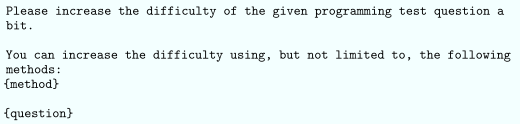
\includegraphics[width=\textwidth]{bilder/kapitel3/evolinst.png}
    \caption{The Evol-Instruct prompt template from \cite{Luo.2024}.}
    \label{fig:evolinst}
\end{figure}

They apply this template to 20.000 samples of the CodeAlpaca dataset\footnote{\url{https://huggingface.co/datasets/theblackcat102/evol-codealpaca-v1} (last visited on 2024-10-31)} to generate their training dataset.
They train iteratively, applying evol-instruct for every epoch and evaluating on HumanEval until they see a decline in pass@1.

At the time of release, WizardCoder was the most prolific open-source code synthesis model, reaching 57\% on HumanEval and 52\% on MBPP, as well as between 33\% and 55\% on DS-1000.


\subsection{Magicoder}
\label{sec:magicoder}
The Magicoder series, introduced by Wei et al. \cite{Wei.2024}, comprise four models trained with the OSS-Instruct approach also first introduced by them.
OSS-Instruct works as follows:
First, a set of seed code snippets is chosen. Wei et al. use Starcoderdata as a base and select 80.000 seed snippets, 40.000 from Python and 5.000 each from C++, Java, TypeScript, Shell, C\#, Rust, PHP and Swift.
A seed snippet in this case refers to 1-15 consecutive lines extracted from a random position in a file of the dataset.
Each seed snippet comes from a different file.
The seed snippets are then applied to the prompt shown in figure \ref{fig:magicoder}.
The prompt in sent to a teacher model, in their case gpt-3.5-turbo-1106, which responds with a problem and a solution.

\begin{figure}[!h]
    \centering
    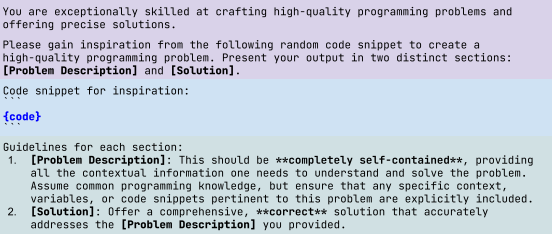
\includegraphics[width=\textwidth]{bilder/kapitel3/magicoder.png}
    \caption{The OSS-Instruct prompt template from \cite{Wei.2024}.}
    \label{fig:magicoder}
\end{figure}

Next, extensive data decontamination is done, disgarding samples that are identical, as well as removing samples containing docstrings, prompts, questions or solutions from HumanEval, MBPP, DS-1000, APPS and GSM8K \cite{Cobbe.2021}.
The final corpus results in around 75.000 rows of data.

To train the model, Wei et al. use CodeLlama-Python-7B and DeepSeek-Coder-Base 6.7 B as base models.
They fine-tune the models for two epochs on the gathered data, giving them two Magicoder models, MagicoderCL and MagicoderDS.
They further fine-tune these into Magicoder$\mathcal{S}$-CL and Magicoder$\mathcal{S}$-DS with the evol-codealpaca-v1 dataset, the same used by WizardCoder, for another two epochs.

These models perform very well on various benchmarks, reaching between 60 (55) and 77 (70) percent on HumanEval(+), between 64 (53) and 76 (64) percent on MBPP(+), as well as results between 28 and 56 percent on DS-1000 and 40 to 58 percent on MultiPL-E.


\subsection{DeepSeekCoder}
\label{sec:deepseek}

The current best-performing open-source model and second best model overall behind GPT-4 on the EvalPlus leaderboard is DeepSeek-Coder -- specifically DeepSeekCoder-V2-Instruct.
The DeepSeekCoder models were originally introduced by Guo et al. \cite{Guo.2024} and improved into the DeepSeekCoder-V2 models five months later \cite{DeepSeekAI.2024}.
The DeepSeekCoder models range from 1. 3B to 33 B and have a base version and an instruct version for each size.
They are trained on 2 T tokens from a dataset created similarly to Starcoderdata, comprising code from 87 languages gathered from GitHub and decontaminated just like Starcoderdata is.
Code comprises 87\% of the training dataset, with the other 13\% consisting of English code-related text and Chinese articles.
DeepSeekCoder aims to develop in the opposite direction of TinyFuncCoder -- where it aims to limit the scope from a file level to a function level, DeepSeekCoder aims to expand the scope from a file level to a repository level.
Training is done both for left-to-right generation and fill-in-the-middle.
On HumanEval, these models achieve between 34.8\% for the base 1.3 B parameter model and 79.3\% on the instruct-33B model.
On MBPP, these two models achieve 46.2\% and 70\% respectively.

The DeepSeekCoder-V2 series comprises models between 1 B and 236 B tokens, marking the first release of an open-source model with a size of over 100 B tokens.
The series was trained on a new dataset comprised of 60\% code, 10\% math and 30\% natural language.
Training is done on 10 T tokens in total and, unlike in the original series, uses reinforcement learning to further improve model performance.
The 236 B parameter V2-Instruct model achieves an impressive 90.2\% on HumanEval and 76.2\% on MBPP+.
\chapter{TinyFuncCoder}
\label{chap:tinycoder}
This chapter presents the contributions made by this thesis, namely the TinyFuncCoder series of \acp{lm} as well as the TinyFuncData dataset.
It explains the dataset creation in section \ref{sec:data}, model architecture in section \ref{sec:architecture} and the training and evaluation processes in sections \ref{sec:training} and \ref{sec:eval} respectively.
A link to the source code is provided in section \ref{sec:repo} alongside an explanation of the repository structure.
Most work in the following sections was done using Jupyter Notebooks\footnote{\url{https://jupyter.org/} (last visited on 2024-10-31)}, a common tool for working with \acp{lm} and data science in general.

\section{Dataset Creation}
\label{sec:data}

This section will describe the process for gathering and preparing the TinyFuncData dataset used to train the TinyFuncCoder series.
The starting point for dataset creation was the deduplicated version of The Stack dataset \cite{Kocetkov.2023}.
It consists of 3 TB of open source GitHub files spread among 358 programming languages.
Further details about this dataset are explained in section \ref{sec:thestack}.

The dataset was loaded into the notebook using \texttt{load\_dataset} from huggingface's \texttt{data}-\texttt{sets} package, using the \texttt{streaming=True} option, which prevents the whole dataset from being downloaded at once, but rather loading it into memory in chunks.
This is done to limit the storage cost of working with large datasets such as The Stack.

Of the columns included in The Stack, the ones used in data extraction were
\begin{itemize}
    \item \texttt{hexsha}: A unique git hash, used as an id
    \item \texttt{lang}: The language of the file
    \item \texttt{max\_stars\_count}: The number of stars of the repository
    \item \texttt{content}: The code in the file
\end{itemize}

Two filters were applied to the dataset:
First, only GitHub's top ten languages as of Q4 2023 were kept \cite{GitHub.2024}, excluding Makefile and Dockerfile as they do not support functions.
To replace them, C\# and Ruby, the languages in 11th and 12th place, were included.
GitHub's top languages were chosen as the data from The Stack is also gathered from it.
As the model is mainly aimed at students, a lot of programming languages are a low priority or entirely obsolete for training.
Instead, focus should be set on the most popular programming languages with which they are most likely to interact.
The language count is set to ten to have a varied amount of popular languages while keeping the scope of the data limited.
Loading the data was done using the \texttt{data\_dir} parameter to stream only the data of each language individually, reducing the amount of data that must be processed drastically.
Next, any file from a repository with a ranking of lower than three stars was excluded.
Stars indicate that the repository has been marked as a favorite and measure popularity.
Three stars is set to exclude repositories with little to no traction.

The next step was to extract all function definitions out of all code files of each language, including the function head, body, and optionally parameters and a docstring.
This is done to train TinyFuncCoder on pure function definitions -- training it on whole code files would introduce overarching knowledge of class or file structures which is not desired.
To extract function definitions, every language had to be treated individually.

\paragraph{Python} was the easiest language to filter.
Since all of the preparation was done in a jupyter notebook, the Python library \texttt{ast} could be used to parse python code from a string into an \ac{ast}.
This \ac{ast} object has built-in functionality to extract all above listed attributes of all functions in a given file.

For all other languages, a \ac{regex} was written to extract the functions from the content string.
\Ac{regex} is a structured language used in pattern recognition and extraction of these patterns from strings.

\paragraph{Languages with a function keyword} including PHP (\texttt{function}), JavaScript (\texttt{function}) and TypeScript (\texttt{function}), but excluding Ruby (\texttt{def}), which will be filtered uniquely, were straightforward to parse, as the \ac{regex} can center around the keyword and be certain to only capture functions.
For example, the \ac{regex} for PHP looks as follows:

\begin{verbatim}
(?<doc>(?:\/\*\*.*?\*\/|\/\/.*?\n)?)\s*

(?<name>(public|protected|private)*\s*function\s+\w+)\s*

(?<args>\((?:[^()]+|(?&args))*\))\s*

(?<body>\{(?:[^{}]+|(?&body))*\})
\end{verbatim}

This regex is seperated into the groups \texttt{(?<doc>)}, \texttt{(?<name>)}, \texttt{(?<args>)} and \texttt{(?<body>)}, corresponding to the four desired elements to extract.
The regex is applied as a whole, with the linebreaks only serving to show each group individually and aiding readability.
Each group besides the last is also capped with optional whitespaces (\texttt{$\backslash$s*}).

The doc group captures a docstring by looking for the start and end of a multiline comment (//* \dots */) or a one-line comment and line break (\texttt{// \dots $\backslash$n}). It is marked as optional with a question mark, as a docstring is not necessarily given.

The name group captures the function definition up to the parameters, including an optional access modifier (\texttt{public}, \texttt{protected} or \texttt{private}), the word \texttt{function} and any user-given name (\texttt{$\backslash$w+}).

The args group captures all arguments given, starting with the opening bracket after the function name and ending with the closing bracket just before the opening curly bracket for the body.
It is the first group where a recursive search has to be done to match an open bracket to the same closing bracket.
This has to be done as if there is a closing bracket anywhere within the parameter list, the \ac{regex} will assume that it ends at that point.
For this reason, all open-close bracket pairs have to be detected, and it must be assumed that the code is well formed (meaning that all opening brackets have to have a closing bracket).
To do this, a recursive block is used that matches either any character that is not an opening or closing bracket, or if a bracket is found, a recursive search of the same pattern within that bracket up to the next closing bracket.
As a function may not have parameters, only one set of brackets is necessary for the function declaration.

Finally, the body group captures the function body from the opening curly bracket to the corresponding closing bracket.
This syntax also requires a recursive search, even moreso than the args block, as the body is much more likely to contain opening and closing brackets within itself, for any nested blocks like \texttt{if}s, \texttt{while}s and more.
These two recursive searches also necessitate the naming of the blocks, as they should be recursively searched individually, not the entire pattern including the docstring and name.

The other two languages require mild variations depending on language specifics but look mostly the same.

\paragraph{Languages without a function keyword} including C, C++, C\#, Java and Shell are slightly more complicated to parse, while functioning broadly the same as the previous group.
The main difference is the name block, as it cannot center around a keyword.
For Java, the \ac{regex} looks as follows:

\begin{verbatim}
    (?<doc>(?:\/\*\*.*?\*\/|\/\/.*?\n)?)\s*
    
    (?<name>(?:public|private|protected)?\s*(?:static)?\s*\w+\s+\w+)\s*
    
    (?<paren>\((?:[^()]+|(?&paren))*\))\s*
    
    (?<brace>\{(?:[^{}]+|(?&brace))*\})
\end{verbatim}

Besides the slightly altered access modifiers, the name is now matched as two words, namely a return type and a user-given name (the easiest example would be \texttt{public static void main}).

This \ac{regex} pattern also matches certain blocks of code that are not function definitions, such as an if-else block -- \texttt{if else (\dots) \{\dots\}} also matches the word-word-args-body pattern.
To combat this, the captured functions then check their name against a list of keywords, removing those that exactly match keywords from these languages.
As keywords are banned from verbatim use as user-defined names, this will filter out all undesired matches without removing real functions.
The regex for the other languages works similarly, with minor adjustments for language specific syntax.

\paragraph{Ruby} was the most complex language to parse as it is the only one besides Python that does not use curly brackets to open and close blocks, without having the benefit of a library like \ac{ast}.
This means Ruby files have to be prepared before they can be given to the \ac{regex}.
As Ruby also uses a function keyword (\texttt{def}), the easiest way to prepare it is to simply insert curly brackets next to all keywords that start and end code blocks and then apply a \ac{regex} like the one already defined.
All keywords that open a block like \texttt{do}, \texttt{class} or \texttt{if} are given an opening bracket directly after the word.
\texttt{end}, the universal signifier of the end of a block, is given a closing bracket directly after it.
The keyword \texttt{def} has to be treated differently, as the curly bracket cannot directly follow the keyword to be matched by the \ac{regex}.
It has to come after the user-given name and the parameter list.
To accomplish this, another \ac{regex} is used to find the entire def-name-args block and add the curly bracket at the end of it.
After all functions are extracted, these added brackets are removed again to keep the code in line with actual Ruby syntax.
\newline

Gathered functions were appended into an array.
When reaching 2.5 M entries, the gathered data was uploaded into a huggingface dataset and the array wiped to prevent a memory overflow.
After all files are parsed, the remaining entries in the array are also uploaded and the data gathering is done.
The resulting dataset has the columns
\begin{itemize}
    \item \texttt{name: string}
    \item \texttt{params: string}
    \item \texttt{body: string}
    \item \texttt{docstring: string}
    \item \texttt{file\_id: string}
    \item \texttt{language: string}
\end{itemize}
where \texttt{file\_id} is the hexsha value of the original dataset.
The uploaded files are saved as parquet files, an efficient way to store data which is recommended for datasets by huggingface\footnote{\url{https://huggingface.co/docs/hub/en/datasets-adding\#which-file-format-should-i-use} (last visited on 2024-10-31)}.
This resulting first iteration of the dataset, TinyFuncData\footnote{\url{https://huggingface.co/datasets/JanDkff/TinyFuncData} (last visited on 2024-10-31)}, has 90 M entries.
Its language distribution is shown in table \ref{tab:default-distribution}.
Creating this initial set took around a week of constant data parsing.

\begin{table}[h!]
    \centering
    \caption{Language distribution of TinyFuncData.}
    \begin{tabular}{|>{\raggedright\arraybackslash}m{4cm}|>{\raggedleft\arraybackslash}m{4cm}|>{\raggedleft\arraybackslash}m{4cm}|}
        \hline
        \textbf{Language} & \textbf{Function Count} & \textbf{Percentage (\%)} \\
        \hline
        Total & 90,214,500 & \makebox[\widthof{90,214,500}][r]{100.0000} \\
        \hline
        Java & 26,157,106 & \makebox[\widthof{26,157,106}][r]{28.9943} \\
        \hline
        C & 16,519,085 & \makebox[\widthof{16,519,085}][r]{18.3109} \\
        \hline
        Python & 16,472,714 & \makebox[\widthof{16,472,714}][r]{18.2595} \\
        \hline
        JavaScript & 14,798,610 & \makebox[\widthof{14,798,610}][r]{16.4038} \\
        \hline
        C\# & 7,446,313 & \makebox[\widthof{7,446,313}][r]{8.2540} \\
        \hline
        PHP & 5,356,751 & \makebox[\widthof{5,356,751}][r]{5.9378} \\
        \hline
        C++ & 1,583,611 & \makebox[\widthof{1,583,611}][r]{1.7554} \\
        \hline
        Ruby & 867,301 & \makebox[\widthof{867,301}][r]{0.9614} \\
        \hline
        TypeScript & 630,778 & \makebox[\widthof{630,778}][r]{0.6992} \\
        \hline
        Shell & 382,231 & \makebox[\widthof{382,231}][r]{0.4237} \\
        \hline
    \end{tabular}
    \label{tab:default-distribution}
\end{table}

Next, the complete dataset is loaded back into the notebook.
As it is considerably smaller than the original, consisting of only ten of the languages and having applied various filters, the whole dataset can be loaded into memory at once.
It is then deduplicated using pandas' \texttt{deduplicate()} method for DataFrames.
The resulting dataset is then also uploaded to huggingface under the name TinyFuncData-dedup\footnote{\url{https://huggingface.co/datasets/JanDkff/TinyFuncData-dedup} (last visited on 2024-10-31)}, with the same 2.5 M chunk size for each uploaded file.
It has a size of 84 M entries.
Its language distribution is shown in table \ref{tab:dedup-distribution}.

\begin{table}[h!]
    \centering
    \caption{Language distribution of TinyFuncData-dedup.}
    \begin{tabular}{|>{\raggedright\arraybackslash}m{4cm}|>{\raggedleft\arraybackslash}m{4cm}|>{\raggedleft\arraybackslash}m{4cm}|}
        \hline
        \textbf{Language} & \textbf{Function Count} & \textbf{Percentage (\%)} \\
        \hline
        Total & 84,101,961 & \makebox[\widthof{84,101,961}][r]{100.0000} \\
        \hline
        Java & 26,077,227 & \makebox[\widthof{26,077,227}][r]{31.0067} \\
        \hline
        Python & 16,248,323 & \makebox[\widthof{16,248,323}][r]{19.3198} \\
        \hline
        JavaScript & 14,088,493 & \makebox[\widthof{14,088,493}][r]{16.7517} \\
        \hline
        C & 11,530,315 & \makebox[\widthof{11,530,315}][r]{13.7099} \\
        \hline
        C\# & 7,400,280 & \makebox[\widthof{7,400,280}][r]{8.7992} \\
        \hline
        PHP & 5,319,176 & \makebox[\widthof{5,319,176}][r]{6.3247} \\
        \hline
        C++ & 1,571,530 & \makebox[\widthof{1,571,530}][r]{1.8686} \\
        \hline
        Ruby & 858,255 & \makebox[\widthof{858,255}][r]{1.0205} \\
        \hline
        TypeScript & 627,370 & \makebox[\widthof{627,370}][r]{0.7460} \\
        \hline
        Shell & 380,992 & \makebox[\widthof{380,992}][r]{0.4530} \\
        \hline
    \end{tabular}
    \label{tab:dedup-distribution}
\end{table}

Next, all rows which do not contain a docstring -- or contain an empty one -- are filtered out, resulting in a final dataset, TinyFuncData-docstring\footnote{\url{https://huggingface.co/datasets/JanDkff/TinyFuncData-docstring} (last visited on 2024-10-31)}.
This is done both to limit the size of the dataset and because the correlation between natural language description and function code is important context for a model that has not previously seen much code data.
This version of the dataset is much smaller, containing only 7.5 M entries.
Its language distribution is shown in table \ref{tab:docstring-distribution}.
\begin{table}[h!]
    \centering
    \caption{Language distribution of TinyFuncData-docstring.}
    \begin{tabular}{|>{\raggedright\arraybackslash}m{4cm}|>{\raggedleft\arraybackslash}m{4cm}|>{\raggedleft\arraybackslash}m{4cm}|}
        \hline
        \textbf{Language} & \textbf{Function Count} & \textbf{Percentage (\%)} \\
        \hline
        Total & 7,535,293 & \makebox[\widthof{7,535,293}][r]{100.0000} \\
        \hline
        Python & 3,987,109 & \makebox[\widthof{3,987,109}][r]{52.9125} \\
        \hline
        C & 991,275 & \makebox[\widthof{991,275}][r]{13.1551} \\
        \hline
        C\# & 810,354 & \makebox[\widthof{810,354}][r]{10.7541} \\
        \hline
        Java & 501,827 & \makebox[\widthof{501,827}][r]{6.6597} \\
        \hline
        JavaScript & 425,887 & \makebox[\widthof{425,887}][r]{5.6519} \\
        \hline
        Ruby & 397,823 & \makebox[\widthof{397,823}][r]{5.2795} \\
        \hline
        PHP & 191,508 & \makebox[\widthof{191,508}][r]{2.5415} \\
        \hline
        C++ & 142,663 & \makebox[\widthof{142,663}][r]{1.8933} \\
        \hline
        Shell & 70,669 & \makebox[\widthof{70,669}][r]{0.9378} \\
        \hline
        TypeScript & 16,178 & \makebox[\widthof{16.178}][r]{0.2147} \\
        \hline
    \end{tabular}
    \label{tab:docstring-distribution}
\end{table}

Finally, for training, all rows with an empty body or a body greater than a length of 20.000 are filtered out, reducing the dataset down to 6.4 M entries.
20.000 is the nearest round number to the 99.95th percentile of all function lengths for TinyFuncCoder-docstring, which is 19.330.
The entire distribution of body line counts and length
is shown in figure \ref{fig:bodydist}.

\begin{figure}[!h]
    \centering
    \begin{minipage}{0.5\textwidth}
        \centering
        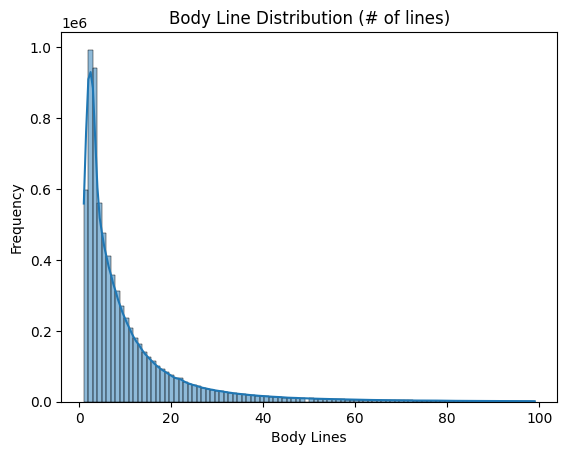
\includegraphics[width=\textwidth]{kapitel4/bodyline.png}
    \end{minipage}\hfill
    \begin{minipage}{0.5\textwidth}
        \centering
        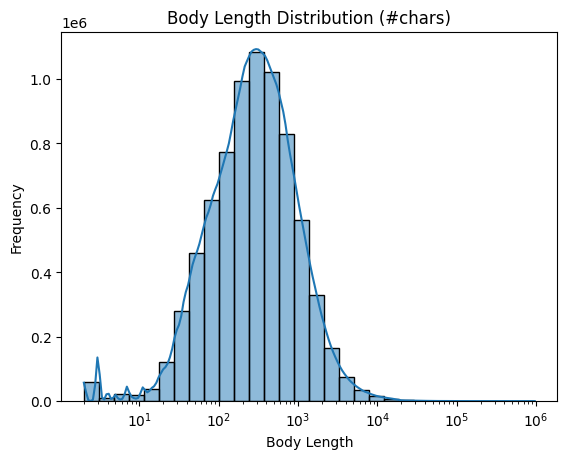
\includegraphics[width=\textwidth]{kapitel4/bodylen.png}
    \end{minipage}
    \caption{Distribution of the number of body lines and body length in TinyFuncData-docstring. The x-axis for the body length distribution is scaled logarithmically.}
    \label{fig:bodydist}
\end{figure}

This version is saved locally as it is the primary version used for training.
Its language distribution is shown in table \ref{tab:final-distribution}.
\begin{table}[h!]
    \centering
    \caption{Language distribution of the final TinyFuncData training set.}
    \begin{tabular}{|>{\raggedright\arraybackslash}m{4cm}|>{\raggedleft\arraybackslash}m{4cm}|>{\raggedleft\arraybackslash}m{4cm}|}
        \hline
        \textbf{Language} & \textbf{Function Count} & \textbf{Percentage (\%)} \\
        \hline
        Total & 6,401,534 & \makebox[\widthof{6,401,534}][r]{100.0000} \\
        \hline
        Python & 3,407,994 & \makebox[\widthof{3,407,994}][r]{53.2371} \\
        \hline
        C & 785,642 & \makebox[\widthof{785,642}][r]{12.2727} \\
        \hline
        C\# & 694,098 & \makebox[\widthof{694,098}][r]{10.8427} \\
        \hline
        Java & 440,217 & \makebox[\widthof{440,217}][r]{6.8767} \\
        \hline
        Ruby & 370,542 & \makebox[\widthof{370,542}][r]{5.7883} \\
        \hline
        JavaScript & 350,351 & \makebox[\widthof{350,351}][r]{5.4729} \\
        \hline
        PHP & 161,854 & \makebox[\widthof{161,854}][r]{2.5284} \\
        \hline
        C++ & 114,124 & \makebox[\widthof{114,124}][r]{1.7828} \\
        \hline
        Shell & 62,993 & \makebox[\widthof{62,993}][r]{0.9840} \\
        \hline
        TypeScript & 13,719 & \makebox[\widthof{13,719}][r]{0.2143} \\
        \hline
    \end{tabular}
    \label{tab:final-distribution}
\end{table}

Figure \ref{fig:language-distributions} shows the percentage changes of each language in relation to the total number of functions for each variant of the dataset.
It can be observed that the most drastic changes occur when filtering by functions with docstring.
The most noticeable change is Python, jumping from under 20\% to over 50\% of data.
Python is perhaps the most prevalent language in \ac{nlp} and \ac{ml} in general.
As will be discussed in chapter \ref{chap:discussion}, Python is also the primary language used for evaluating model code synthesis performance.
This could imply that a lot of Python data found on GitHub is also \ac{ai}-generated, which could also explain why so much Python code has a docstring.
\ac{ai} code is typically heavily commented.
This raises questions about the merit of training a \ac{lm} on \ac{lm}-generated data for this use case, but this topic falls outside the scope of this thesis.

Also notable is that JavaScript and especially Java have a sharp dropoff when filtering for docstrings, with Java dropping by around 15\% and JavaScript by 10\%.
This is surprising, especially considering Java's robust docstring support.

Finally, it should be noted that the ordering of the languages for the original dataset does not match GitHub's ranking from which the languages were selected.
This is most likely due to the fact that some languages are much more function reliant than others.
This may explain some of the previous observations as well -- a language like Java is almost entirely built on functions, and many of them might be simple enough as to need no explicit documentation (like a getter), not to mention main functions.
Languages like Python, which often have logic outside of functions, may have docstrings more commonly as functions are rarer and used more purposefully.
This does not explain why JavaScript, which can also place logic outside of functions, has a steep dropoff as well.

% total amount figure
\begin{comment}
\begin{figure}
    \centering
    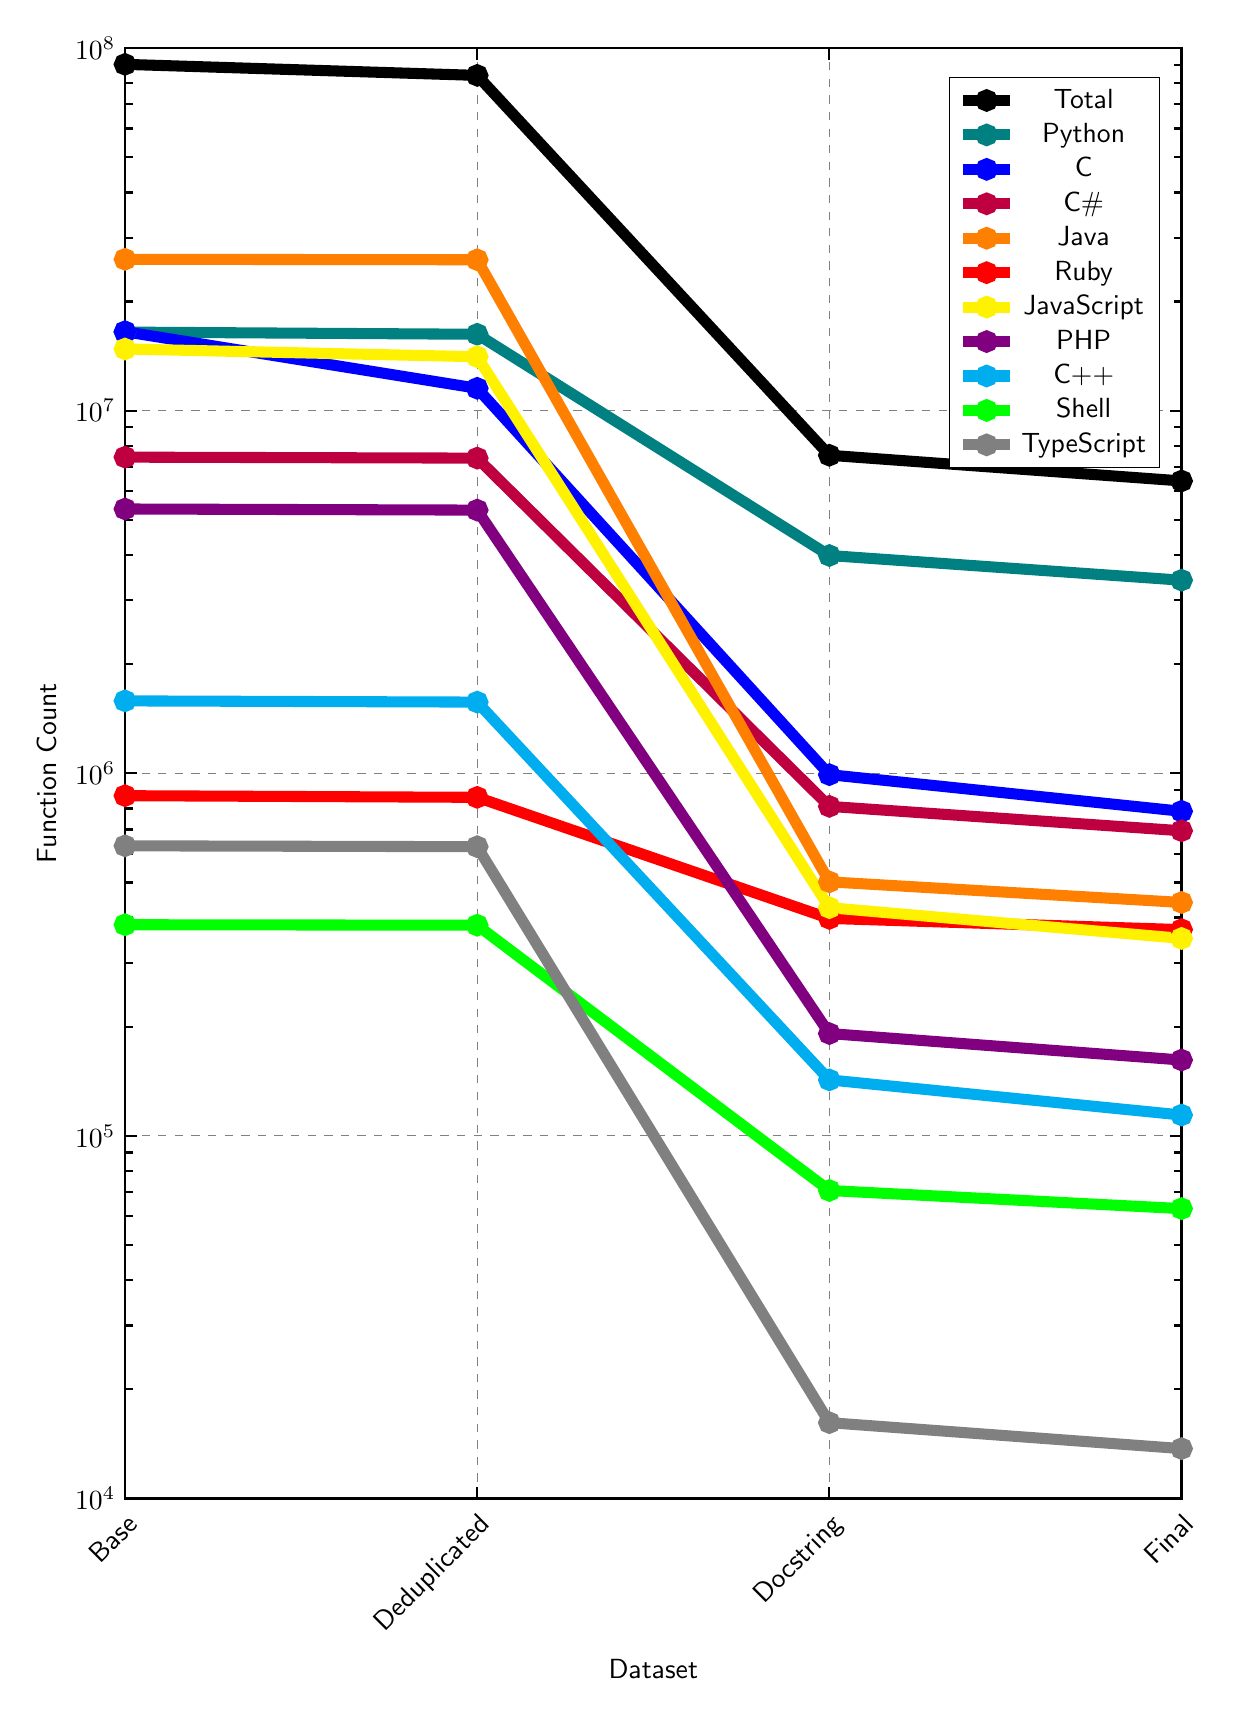
\begin{tikzpicture}
        \begin{axis}[
            width=15cm, height=20cm,
            xlabel={Dataset},
            ylabel={Function Count},
            xtick={1,2,3,4},
            xticklabels={Base, Deduplicated, Docstring, Final},
            xticklabel style={rotate=45, anchor=north east},
            ymode=log,
            log basis y={10},
            ymin=1e4, ymax=1e8,
            grid=major,
            every axis plot/.append style={thick, mark=*, line width=4pt},
            clip=false,
            axis line style={thick, black},
            tick style={thick, black},
            grid style={dashed, gray},
            %legend style={at={(1.05,1)},anchor=north west},
            %legend cell align={left},
            font=\sffamily,
            xmin=1,
            xmax=4
        ]
        % Data for each language
        \addplot[color=black,mark=*] coordinates {(1,90214500) (2,84101961) (3,7535293) (4,6401534)};
        %\node[right] at (axis cs:4.2,6401534) {Total};
        \addlegendentry{Total};
    
        \addplot[color=teal,mark=*] coordinates {(1,16472714) (2,16248323) (3,3987109) (4,3407994)};
        %\node[right] at (axis cs:4.2,3407994) {Python};
        \addlegendentry{Python};
    
        \addplot[color=blue,mark=*] coordinates {(1,16519085) (2,11530315) (3,991275) (4,785642)};
        %\node[right] at (axis cs:4.2,785642) {C};
        \addlegendentry{C};
    
        \addplot[color=purple,mark=*] coordinates {(1,7446313) (2,7400280) (3,810354) (4,694098)};
        %\node[right] at (axis cs:4.2,694098) {C\#};
        \addlegendentry{C\#};

        \addplot[color=orange,mark=*] coordinates {(1,26157106) (2,26077227) (3,501827) (4,440217)};
        %\node[right] at (axis cs:4.2,440217) {Java};
        \addlegendentry{Java};
    
        \addplot[color=red,mark=*] coordinates {(1,867301) (2,858255) (3,397823) (4,370542)};
        %\node[right] at (axis cs:4.2,370542) {Ruby};
        \addlegendentry{Ruby};

        \addplot[color=yellow,mark=*] coordinates {(1,14798610) (2,14088493) (3,425887) (4,350351)};
        %\node[right] at (axis cs:4.2,350351) {JavaScript};
        \addlegendentry{JavaScript};

        \addplot[color=violet,mark=*] coordinates {(1,5356751) (2,5319176) (3,191508) (4,161854)};
        %\node[right] at (axis cs:4.2,161854) {PHP};
        \addlegendentry{PHP};

        \addplot[color=cyan,mark=*] coordinates {(1,1583611) (2,1571530) (3,142663) (4,114124)};
        %\node[right] at (axis cs:4.2,114124) {C++};
        \addlegendentry{C++};

        \addplot[color=green,mark=*] coordinates {(1,382231) (2,380992) (3,70669) (4,62993)};
        %\node[right] at (axis cs:4.2,62993) {Shell};
        \addlegendentry{Shell};

        \addplot[color=gray,mark=*] coordinates {(1,630778) (2,627370) (3,16178) (4,13719)};
        %\node[right] at (axis cs:4.2,13719) {TypeScript};
        \addlegendentry{TypeScript};
        \end{axis}
    \end{tikzpicture}
    \caption{Language distributions among the four versions of the dataset. The y-axis is scaled logarithmically.}
    \label{fig:language-distributions}
\end{figure}
\end{comment}

% percentage amount figure
\begin{figure}[H]
    \centering
    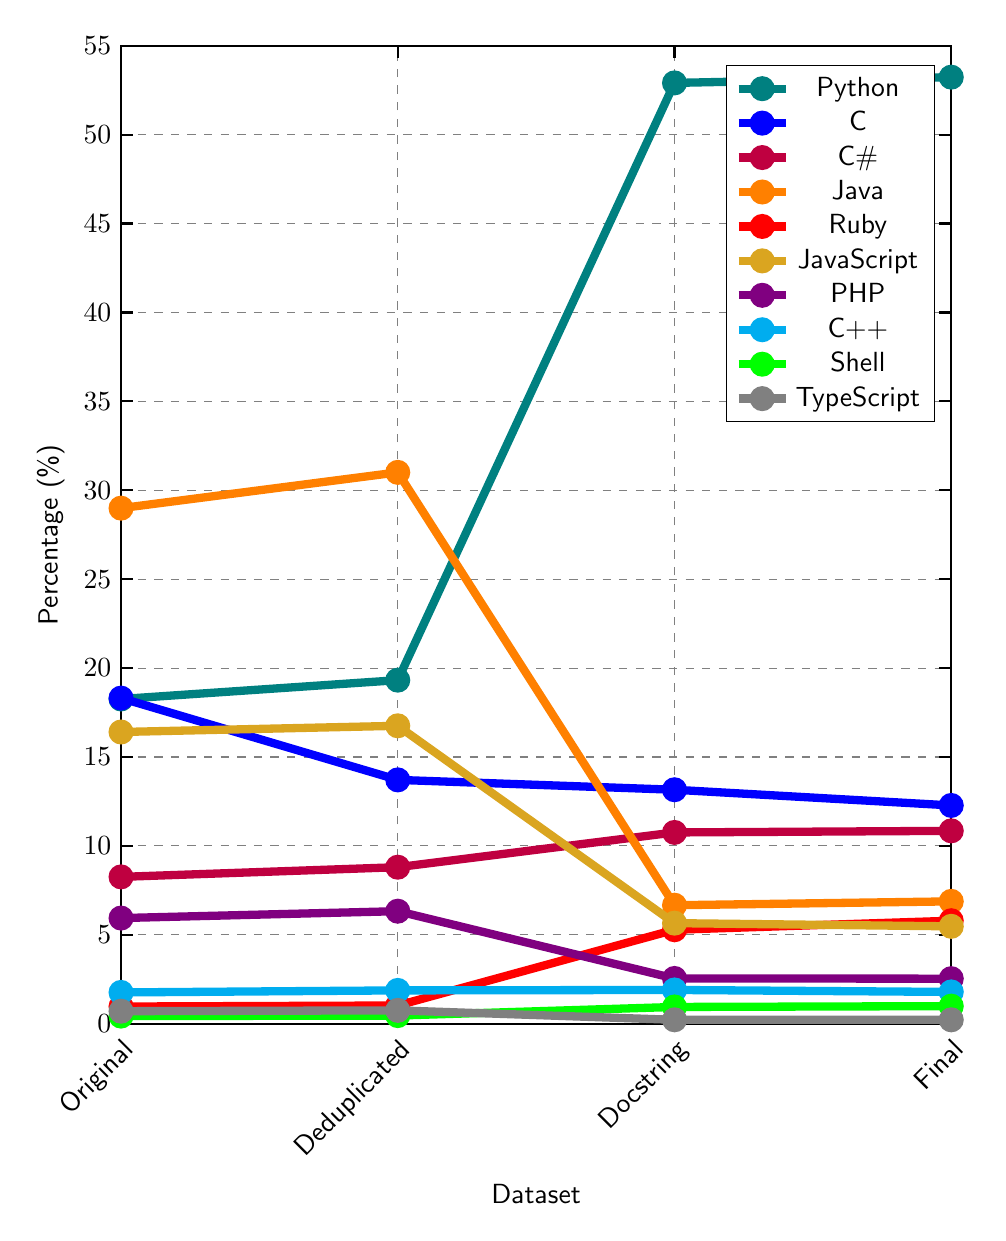
\begin{tikzpicture}
        \begin{axis}[
            width=\textwidth, height=14cm,
            xlabel={Dataset},
            ylabel={Percentage (\%)},
            xtick={1,2,3,4},
            xticklabels={Original, Deduplicated, Docstring, Final},
            xticklabel style={rotate=45, anchor=north east},
            ymode=linear,
            ymin=0, ymax=55,
            xmin=1, xmax=4,
            grid=major,
            every axis plot/.append style={thick, mark=*, line width=3pt},
            clip=false,
            clip mode=individual,
            axis line style={thick, black},
            tick style={thick, black},
            grid style={dashed, gray},
            font=\sffamily
        ]
    
        \addplot[color=teal, mark=*, mark size=3pt] coordinates {(1,18.2595) (2,19.3198) (3,52.9125) (4,53.2371)};
        \addlegendentry{Python};
    
        \addplot[color=blue, mark=*, mark size=3pt] coordinates {(1,18.3109) (2,13.7099) (3,13.1551) (4,12.2727)};
        \addlegendentry{C};

        \addplot[color=purple, mark=*, mark size=3pt] coordinates {(1,8.2540) (2,8.7992) (3,10.7541) (4,10.8427)};
        \addlegendentry{C\#};

        \addplot[color=orange, mark=*, mark size=3pt] coordinates {(1,28.9943) (2,31.0067) (3,6.6597) (4,6.8767)};
        \addlegendentry{Java};

        \addplot[color=red, mark=*, mark size=3pt] coordinates {(1,0.9614) (2,1.0205) (3,5.2795) (4,5.7883)};
        \addlegendentry{Ruby};
    
        \addplot[color=Goldenrod, mark=*, mark size=3pt] coordinates {(1,16.4038) (2,16.7517) (3,5.6519) (4,5.4729)};
        \addlegendentry{JavaScript};
    
        \addplot[color=violet, mark=*, mark size=3pt] coordinates {(1,5.9378) (2,6.3247) (3,2.5415) (4,2.5284)};
        \addlegendentry{PHP};
    
        \addplot[color=cyan, mark=*, mark size=3pt] coordinates {(1,1.7554) (2,1.8686) (3,1.8933) (4,1.7828)};
        \addlegendentry{C++};
    
        \addplot[color=green, mark=*, mark size=3pt] coordinates {(1,0.4237) (2,0.4530) (3,0.9378) (4,0.9840)};
        \addlegendentry{Shell};
    
        \addplot[color=gray, mark=*, mark size=3pt] coordinates {(1,0.6992) (2,0.7460) (3,0.2147) (4,0.2143)};
        \addlegendentry{TypeScript};
    
        \end{axis}
    \end{tikzpicture}
    \caption{Language distributions among the four versions of the dataset.}
    \label{fig:language-distributions}
\end{figure}

\section{Architecture}
\label{sec:architecture}

To finetune a \ac{llm} on a dataset as large as TinyFuncData on limited hardware, many efficiency-boosting tactics have to be used when designing the model and training architecture.
This section will explain the entire architecture for fine-tuning on the TinyFuncData-docstring dataset in detail, explaining all concepts, libraries and parameters used, as well as their purpose.
Many of the libraries used come from the huggingface hub\footnote{\url{https://huggingface.co/} (last visited on 2024-10-31)}, a website focused on hosting \acp{lm}, datasets for model training, \ac{nlp} libraries and documentation, as well as a space for community discussions surrounding the topic.
It hosts over a million models and over 235.000 datasets and is free for anyone to use, download from, and upload their own work to.
\enquote{The hub} will be used interchangably as a shorthand for the full name.

\paragraph{Data Loading:}
The dataset is loaded using the \texttt{load\_dataset()} function from huggingface's \texttt{datasets} library, which can download datasets hosted on the site.
The dataset was saved on the hub during creation, and using this function is the intended way of loading it into a notebook.


\paragraph{Tokenization:}
The \texttt{AutoTokenizer}\footnote{\url{https://huggingface.co/docs/transformers/v4.42.0/en/model_doc/auto\#transformers.AutoTokenizer} (last visited on 2024-10-31)} from huggingface's \texttt{transformers} library is used for tokenization.
\texttt{AutoTokenizer.from\_pretrained()} is used to create a tokenizer for each base model used.
This class automatically loads the appropriate tokenizer for a provided model name.

\paragraph{Configs:}
Two configs are used in order to train the model with \ac{qlora}:
a \texttt{BitsAndBytes\\Config}\footnote{\url{https://huggingface.co/docs/transformers/en/main_classes/quantization\#transformers.BitsAndBytesConfig} (last visited on 2024-10-31)} from \texttt{transformers}, and a \texttt{LoraConfig}\footnote{\url{https://huggingface.co/docs/peft/en/package_reference/lora\#peft.LoraConfig} (last visited on 2024-10-31)} from the \texttt{peft} library.

The \texttt{BitsAndBytesConfig} is used for quantization of models, and it is later passed as an argument when loading the model.
The most important parameters are as follows:
\begin{itemize}
    \item \texttt{load\_in\_4bit} is set to \texttt{True}, causing the model to be 4-bit quantized, as explained in section \ref{sec:qlora}. It does this by replacing the models linear layers with \texttt{bitsandbytes}' quantized layers.
    \item \texttt{bnb\_4bit\_compute\_dtype} is set to \texttt{bfloat16} (brain floating point 16), which changes the computation type, speeding up calculations.
    \item \texttt{bnb\_4bit\_use\_double\_quant} is set to \texttt{True}, causing nested quantization for quantized parameters, saving even more space per parameter.
\end{itemize}

The \texttt{LoraConfig}'s purpose is to turn the model into a \ac{peft} model through the \texttt{get\_peft\_\\model()} function, a model that utilizes \ac{lora}.
The most important parameters are as follows:
\begin{itemize}
    \item \texttt{r}, the rank, is set to 64.
    \item \texttt{lora\_alpha}, used for \ac{lora} parameter scaling, is set to 16. Scaling is used to weigh the new \ac{lora} parameters against the old model parameters. Rank and alpha were decided on after some hyperparameter testing, as explained in section \ref{sec:pretrain}.
    \item \texttt{lora\_dropout} acts like regular dropout and is set to 0.1, a standard value.
\end{itemize}

\paragraph{Model Initialization:}
The different models are loaded using \texttt{transformers}' \texttt{AutoModel\\ForCausalLM.from\_pretrained()}\footnote{\url{https://huggingface.co/docs/transformers/v4.42.0/en/model_doc/auto\#transformers.AutoModelForCausalLM} (last visited on 2024-10-31)}, a class and function designed to easily load pretrained models directly from huggingface for causal language modeling -- predicting the next token given a sequence of tokens.
The most important parameters are as follows:
\begin{itemize}
    \item \texttt{model\_name} is the base models name
    \item \texttt{quantization\_config} takes the \texttt{BitsAndBytesConfig} created earlier.
    \item \texttt{device\_map} is set to \texttt{"auto"} to automatically distribute the model across the server's \acp{gpu}.
\end{itemize}

After initializing the model, \texttt{peft}'s \texttt{prepare\_model\_for\_kbit\_training()} and \texttt{get\_\\peft\_model()} are called to transform the model into a \ac{peft} model.
This is also where the \texttt{LoraConfig} is given to the model.
The first function prepares the model for low-rank training by converting model weights.
The second wraps the model with the new \ac{lora} layers that will be trained, according to the given configuration.

\paragraph{Data Collation:}
for data collation, a \texttt{DataCollatorForLanguageModeling}\footnote{\url{https://huggingface.co/docs/transformers/en/main_classes/data_collator\#transformers.DataCollatorForLanguageModeling} (last visited on 2024-10-31)} from \\\texttt{transformers} is used.
The \texttt{mlm} flag is set to \texttt{False} to disable masked training due to its high resource cost.

\section{Training}
\label{sec:training}

This section describes the training process used to fine-tune the TinyFuncCoder models.
Section \ref{sec:setup} shows the libraries and parameters used in the training pipeline.
Section \ref{sec:hardware} gives a brief explanation of the hardware used for training.
Section \ref{sec:pretrain} describes the various steps in creating the training pipeline, culminating in the final pipeline explained in \ref{sec:finaltrain}.
Figure \ref{fig:architecture} shows a full diagram of the used architecture and training pipeline.
The details of its component are described in section \ref{sec:architecture} as well as the upcoming sections.

\begin{figure}[H]
    \centering
    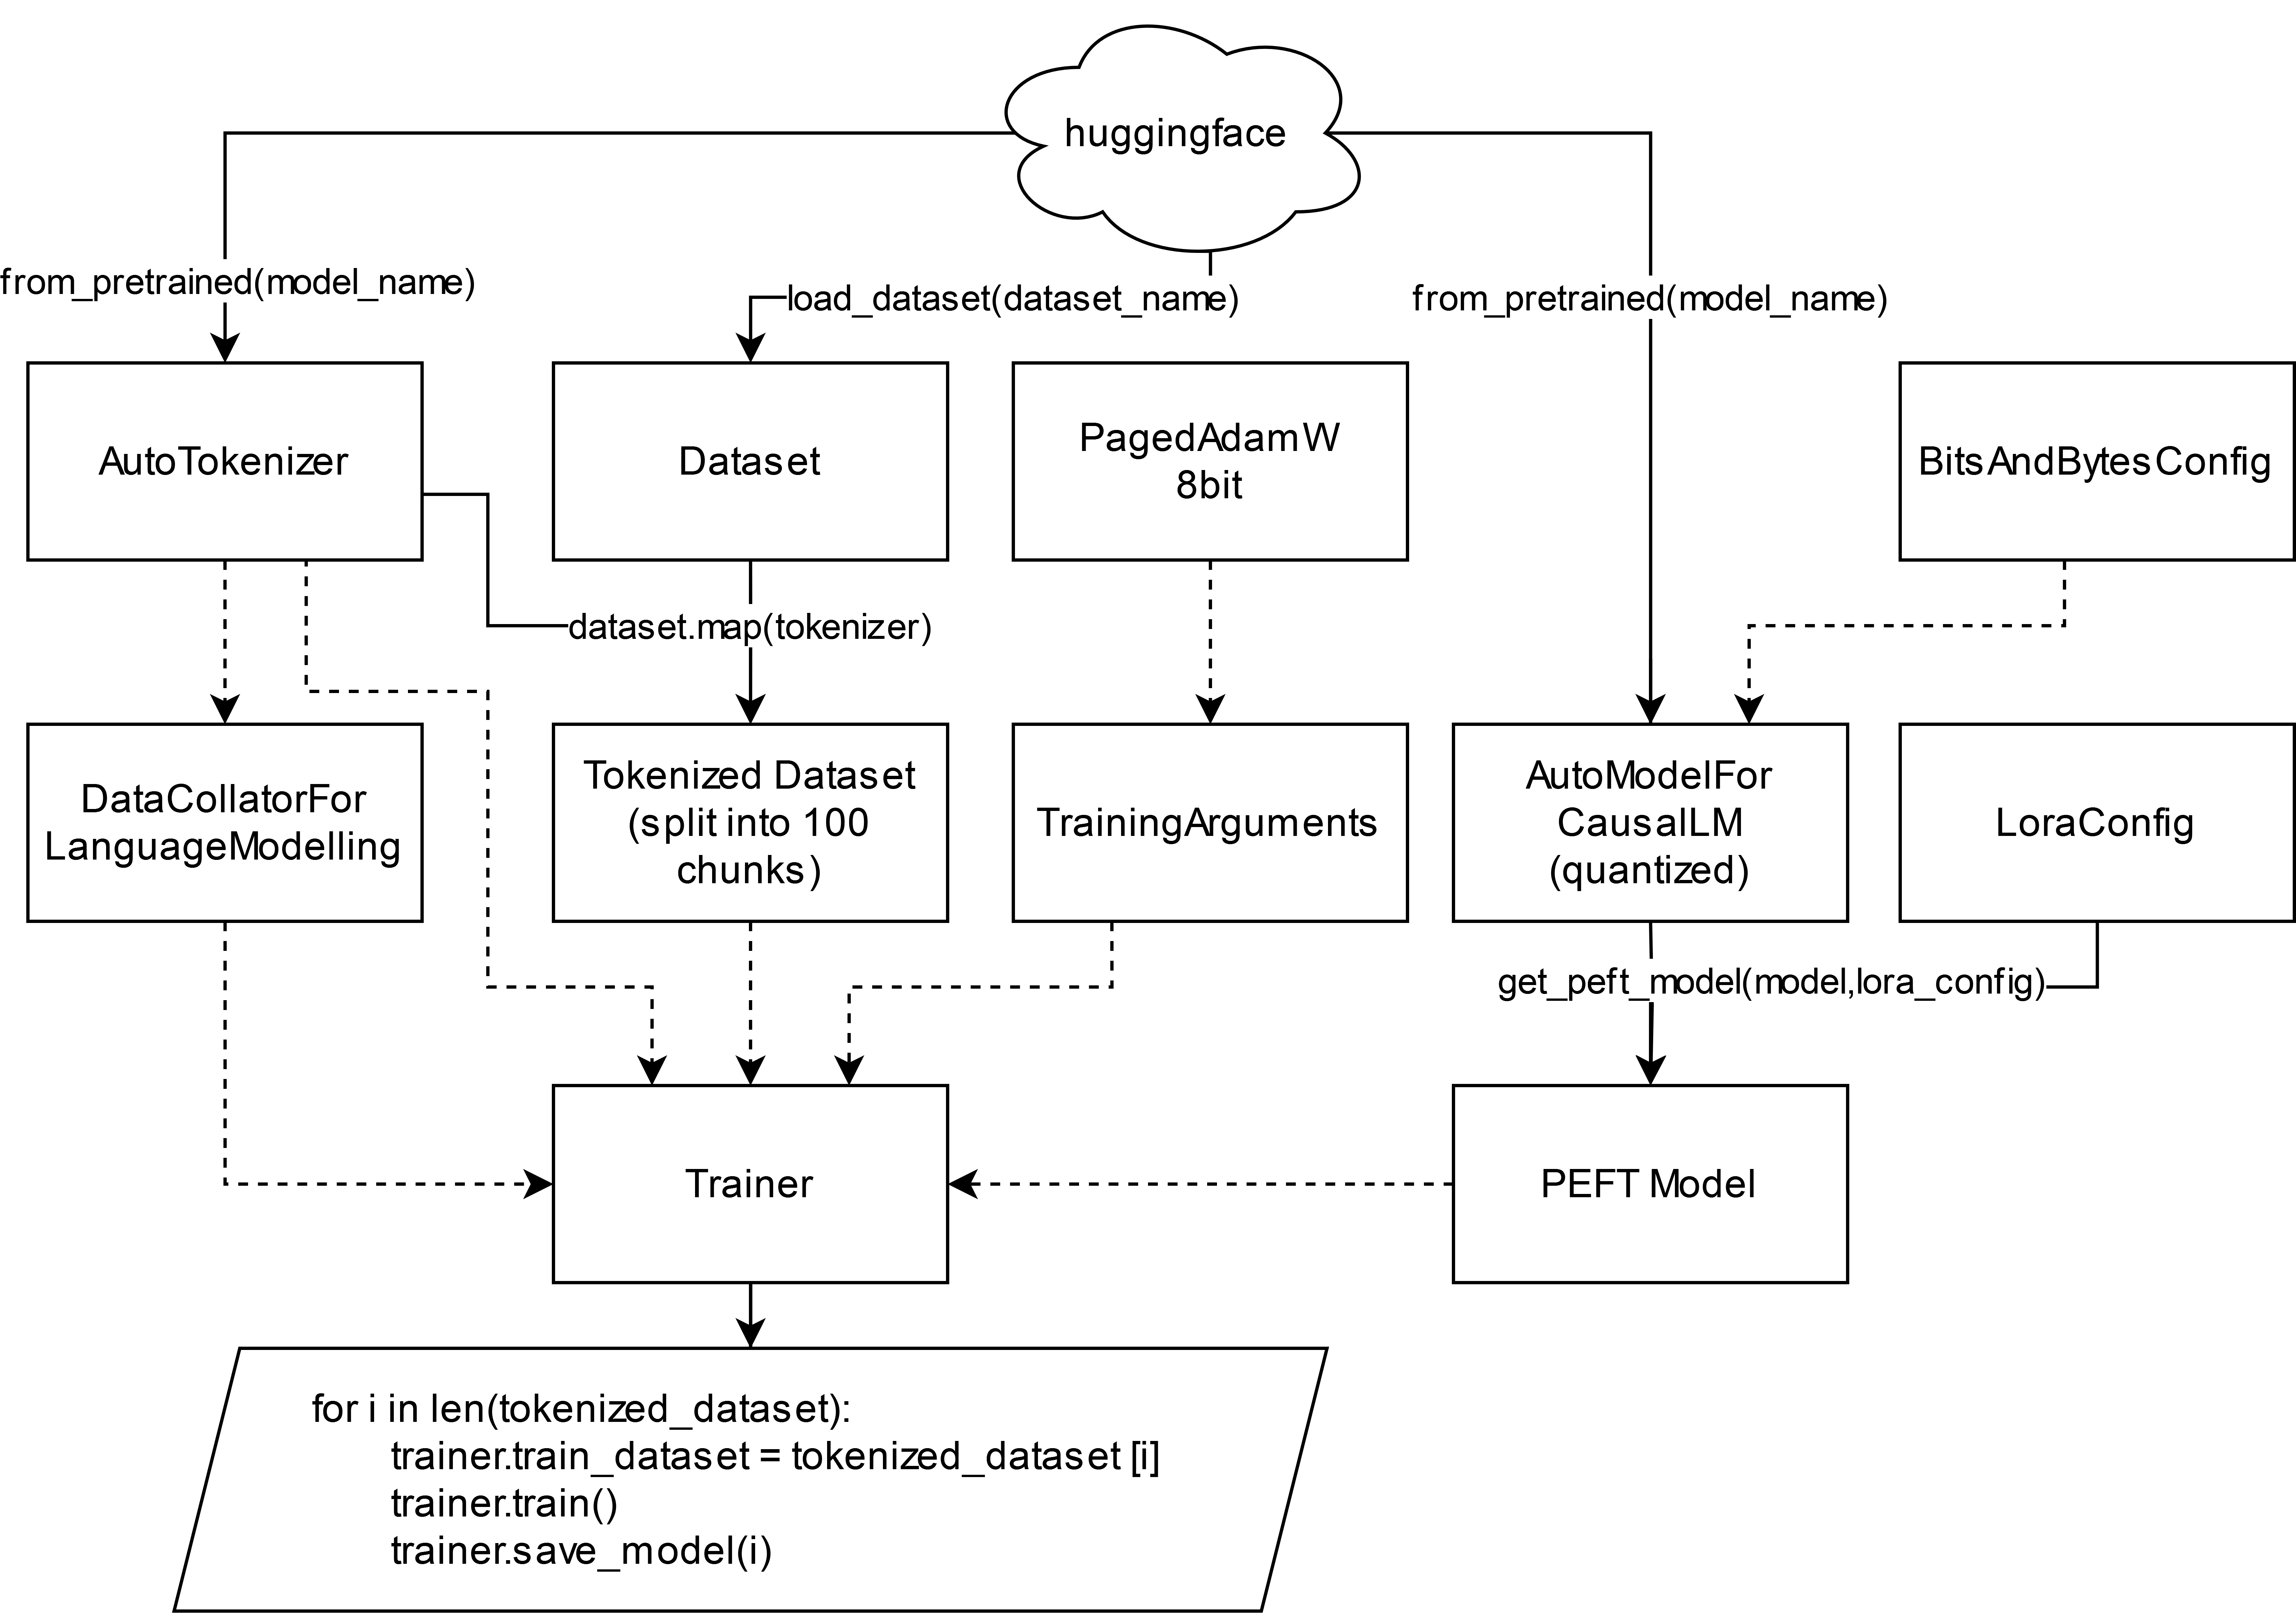
\includegraphics[width=\textwidth]{bilder/kapitel4/architecture.png}
    \caption{The full training pipeline of TinyFuncCoder. Boxes indicate object instances. Solid arrows indicate function calls using the connecting instances. Dotted arrows indicate use of an instance as a variable for another object. Arrows coming from the cloud indicate loading data for instancing from the huggingface hub.}
    \label{fig:architecture}
\end{figure}

\subsection{Training Setup}
\label{sec:setup}
For training the model, \texttt{transformers}' \texttt{Trainer}\footnote{\url{https://huggingface.co/docs/transformers/en/main_classes/trainer\#transformers.Trainer} (last visited on 2024-10-31)} and \texttt{TrainingArguments}\footnote{\url{https://huggingface.co/docs/transformers/en/main_classes/trainer\#transformers.TrainingArguments} (last visited on 2024-10-31)} are used, which allow for easy configuration of a training loop for the model.

\paragraph{Training Arguments:}
The most important training arguments are as follows:
\begin{itemize}
    \item \texttt{per\_device\_\{train/eval\}\_batch\_size}: The batch size for training and evaluation. Both are set to 1, as crashes because of memory issues were the biggest concern during training.
    \item \texttt{gradient\_accumulation\_steps}: The number of steps before a backpropagation is done through the model. This is set to 8 to further reduce memory cost by limiting backpropagation.
    \item \texttt{dataloader\_num\_workers}: This denotes the number of subprocesses to be used in data loading. This is set to 4.
    \item \texttt{learning\_rate}: The learning rate is set to 1e-5.
    \item \texttt{fp16}: Setting this to True will enable 16-bit precision training, rather than the default 32-bit.
    \item \texttt{optim}: The optimizer used by the model. In this case, a PagedAdamW optimizer, which is more memory-efficient than a regular AdamW, is used.
    \item \texttt{\{eval/logging/save\}\_strategy}: is set to \texttt{"steps"} for \texttt{eval}, so that results can be seen at every x training steps. As the dataset is large and training takes long, setting it to \texttt{"epoch"} would not provide sufficient information to monitor and evaluate the training process.
    Important to note is that a step is counted as a backwards pass when using gradient accumulation, so this is only done once each \texttt{\{eval/logging/save\}\_steps $\cdot$ gradient\_accumulation\_steps}. Eval is set to 3200, or half of an epoch, logging arbitrarily to 250, and saving to once per epoch.
    \item \texttt{seed}: The seed used for random number generation, assuring reproducability of the results. It is set to 42.
\end{itemize}

\paragraph{Trainer:}
Finally, to begin training, the \texttt{Trainer} class is initialized with the other objects that have been created so far: the model, training arguments, training and evaluation datasets and the tokenizer and data collator.
Once the trainer has been created, \texttt{trainer.train()} can be called to begin fine-tuning the model.
For TinyLlama, new parameters of around 1.44\% of the total amount of model parameters are trainable using the LoraConfig described earlier.


\subsection{Hardware and Software}
\label{sec:hardware}
Dataset creation, training and evaluation were split between two devices: a personal computer used mainly for filtering the function definitions from The Stack, as well as evaluating the results generated by the models.
Model training, further dataset filtering and result generation was done on a server provided and maintained by Prof. Dr. Oliver Hummel of the faculty of computer science, University of Applied Sciences Mannheim as part of TransforMA\footnote{\url{https://www.hs-mannheim.de/die-hochschule/forschung-und-transfer/transforma.html} (last visited on 2024-31-10)}.
Table \ref{tab:architecture} shows the specs of both machines.

Connection to the TransforMA server was achieved through VS Code's Remote-SSH extension, opening an SSH tunnel to the server.
A VPN connection to the university is also required.
Code was run in VSCode's Jupyter extension.

To prevent having to keep a connection to the server, as it automatically closes after a timeout period, most time intensive tasks were done using papermill\footnote{\url{https://papermill.readthedocs.io/en/latest/} (last visited on 2024-10-31)}.
To this end, the command
\begin{lstlisting}[language=bash]
    nohup papermill notebook.ipynb notebook-out.ipynb 1>>notebook.out 2>> notebook.out &
\end{lstlisting}
is run, executing the notebook using papermill while using nohup to force the code to keep running even when the connection is closed.
1>{}> and 2>{}>, referring to the standard and error output, are saved in <notebook>.out while <notebook>-out.ipynb is a copy of the original notebook that is updated close to real time with the cell outputs.

\begin{table}[!h]
    \centering
    \caption{Specs of the machines used in the creation of TinyFuncCoder and TinyFuncData.}
    \begin{tabular}{l|l|l|l|l}
        \hline
        & \textbf{CPU} & \textbf{RAM} & \textbf{GPU} & \textbf{GPU RAM} \\
        \hline
        \textbf{PC} & $1\times$ AMD Ryzen 5 & 16 GB & $1\times$ NVIDIA GeForce & $1\times$ 8 GB \\
        & 5600X 6-Core & & RTX 3060 Ti & \\
        \hline
        \textbf{TransforMA} & $48\times$ AMD EPYC & 256 GB & $2\times$ NVIDIA GeForce & $2\times$ 24 GB \\
        & 7443P 24-Core & & RTX 4090 & \\
        \hline
    \end{tabular}
    \label{tab:architecture}
\end{table}

\subsection{Exploratory Training}
\label{sec:pretrain}

Creation of the TinyFuncCoder series was an iterative process of testing multiple approaches to maximize model performance within the constraints of the hardware.
The results of the approaches will be more thoroughly presented in section \ref{sec:eval} and only briefly mentioned here to explain decisions made for each iteration.
Every model checkpoint was evaluated on HumanEval and HumanEval+ to compare performance.
While this is not an exhaustive comparison, it is a comparatively quick way to assess model performance, as using multiple metrics would take much longer and slow down the speed of iteration.
HumanEval was chosen as it is the most popular and relatively quick to generate for. It takes around 45 minutes to fully generate all answers, and under a minute to assess them. TinyLlama was chosen for testing because it is the smallest of the models considered (see section \ref{sec:basemodels}) and thus quickest to fine-tune.

The first step to fine-tuning the model was deciding on how to format the functions.
A simple first choice is simply feeding the entire function into the model, in the order \enquote{docstring -- function head -- function body}.
To help the model use appropriate syntax, a custom line is added to the start of the docstring specifying the language in which the function is written.
This simplistic approach quickly proved error-prone, as when using a model trained this way it will not stop generating when the function end is reached, instead generating more comments or functions or even text attempting to explain what the function does.
To stop this behaviour, a start and end token are added before the first and at the end of the last line of all training data.
These are \enquote{<func>} and \enquote{<$\backslash$func>}, similar to opening and closing tags for HTML. 
Tags of a similar form are often used in training.
For example, Gemma uses the pad token \enquote{\texttt{<pad>}}, Magicoder uses \enquote{\texttt{<|end\_of\_sentence|>}} and WizardCoder uses \enquote{\texttt{[PAD]}}.
This way, the model learns a starting point for all functions, the comment clarifying the language, as well as an end point for each of the training functions.
Allowing the model to generate an end token opens the possibility to ignore all generated text past that point, resulting in better results.

Fine-tuning on the entire dataset was not feasible, as even with optimized settings, it was projected to take 300 hours and typically crashed due to memory issues before then.
Instead, multiple subsets of 1\% size were created.
Half of these were done with stratified sampling by language, meaning an equal number of rows for each language, the other half with a fixed size of .1\% of the total per language.
This splitting is done with pandas'
These were split 80/20 into training and validation data, with validation being further split into a valdiation and testing set.
Attempting to use the testing set always resulted in a crash and the second split was eventually deemed unnecessary because the model would be tested on the metrics introduced in \ref{sec:metrics}.
Training and evaluating with these sets of 1\% took around 9.5 hours each for one epoch.
Attempting to train on a 5\% stratified subset also resulted in a crash due to memory issues.

As all of these produced comparably middling results, a next attempt was to fine-tune multiple epochs on a single one of these subsets, which often yielded worse performance. Experimenting with different \ac{lora} parameters also worsened performance on the same data.

This lead to the decision to instead attempt to fine-tune on multiple subsets of the full dataset, swapping each epoch to see more functions to learn from.
Trying to build an architecture to facilitate a single training loop swapping out its dataset for every epoch took four iterations:

For all iterations, a loop was run over the desired epoch count (100).
At this point, the testing set was discarded because it was not being used, increasing the size of the validation set to a full 20\% of the total.
In the first attempt, all relevant classes to the model (tokenizer, training arguments, trainer, model, etc.) were created inside of the training loop.
The dataset was also split at runtime.
At the end of the epoch, a checkpoint was saved, which was used with the trainer's \texttt{resume\_from\_checkpoint} flag to continue training.
However, this changes the training arguments and dataset of the trainer, changing the desired outcome.
Datasets were generated as a stratified sample by language with a seed corresponding to the epoch number.

For the second iteration, most classes were initialized outside of the loop, with only the trainer and dataset being created inside.
This has the desired effect of changing the dataset, but the trainer saves other important values during training which are continuously reset this way.

In the third attempt, the trainer was given a callback function that attempted to change the dataset at the start of each epoch.
This did not work because the trainer kept training before the dataset had time to finish loading.

Finally, the dataset was split into 100 evenly-sized stratified chunks which were saved on disk.
This prevents overlap in the random sampling and allows fast loading because it does not first have to be split at runtime.
The dataset is then simply swapped out through a property call on the trainer at the start of the training loop.
This allows the trainer to be created outside of the loop, retaining its learned properties.
For all iterations, the remnants of dataset loading had to be manually deleted using Python's garbage collection library \texttt{gc}.
A big problem was also setting the training arg's epoch counter.
The issue was that setting an epoch amount of one and saving and resuming from checkpoints did not work because the model thought it was done training (1/1 had been completed).
Setting it higher made the trainer train multiple epochs on the same data.
Previous approaches often could not account for this discrepancy.
Attempts were even made to dynamically alter the epoch counter for every new dataset.
In this fourth iteration, the configuration allows setting the epoch count to one because checkpoints are not being used, solving the issue. With around 9.5 hours per epoch, the total time spent training was around 180 hours, or 7.5 days.

\subsection{Final Training}
\label{sec:finaltrain}

The final training for the TinyFuncCoder series was done on TinyLlama-1.1B-Chat-v1.0 and TinyLlama\_v1.1, resulting in TinyFuncCoder-v1.0 and TinyFuncCoder-v1.1.
All other models on which training was considered (described in section \ref{sec:basemodels}) ran into issues that could not be resolved, including problems with model and data distribution to devices, matrix size mismatches or errors that gave no specific information at all.
Both were trained with the final, successful approach described in section \ref{sec:pretrain}, initially iterating over all 100 chunks of data.
The training was still prone to crashes due to memory issues.
These were consistent and happened at the same points of the same chunks every time, and the offending chunks were simply skipped.
Training was resumed from the most recent checkpoint on the next chunk.
Due to time constraints, training per model was limited to 25 chunks, exactly a quarter of the entire set.
These chunks are 0, 1, 2, 5, 6, 7, 8, 10, 12, 14, 15, 16, 17, 18, 21, 24, 26, 29, 30, 31, 32, 33, 34, 35 and 37, counting up from 0 and skipping all chunks with memory issues. V1.1 additionally skips chunk 21 due to memory issues.
During training for v1.0, a few epochs were erroneously trained starting from the wrong checkpoint.
This was eventually discovered and the model retrained from the proper checkpoint.
Training loss remained close to 1.3 for the entirety of training, as will be more closely examined in \ref{sec:loss}.

Training a single epoch on v1.0, including two evaluations, took around 9.5 hours.
Training v1.1 was initially started with identical parameters, which resulted in a training time of around 2.5 hours.
During this training, the loss jumped to over nine from around two in the third epoch.
Training was restarted, loading the model in 8-bit quantization instead of 4-bit, which improved the loss drastically and prevented it from rapidly increasing, but also increased the training time of an epoch to around twelve hours as much of the \ac{qlora} costs and benefits are reduced with the change to a larger data type.
This puts the total training time for v1.0 to 237.5 hours and for v1.1 to 288 hours, around 10 days and 12 days respectively.
This is ignoring time spent restarting training or the erroneously trained chunks.

\section{Evaluation}
\label{sec:eval}

For the evaluation of the test steps, the EvalPlus GitHub\footnote{\url{https://github.com/evalplus/evalplus} (last visited on 2024-10-31)} repository was downloaded and its code used to generate and evaluate the HumanEval and HumanEval+ benchmarks.
To generate and run the code, a Docker container was used to prevent the potentially harmful code generated by a \ac{lm} to be run without protection.
To this end, VSCode's \ac{wsl} support was used, which in turn connected to Docker Desktop through its built in support for \ac{wsl}.
The command
\begin{lstlisting}[language=bash]
    docker run -v \$(pwd):/app ganler/evalplus:latest --dataset humaneval --samples samples.jsonl
\end{lstlisting}
was used, taken directly from the EvalPlus GitHub page.
To run this command on Windows, \texttt{\$(pwd)} can be swapped for \texttt{\$\{PWD\}}.

For a full evaluation run, the Bigcode Evaluation Harness code\footnote{\url{https://github.com/bigcode-project/bigcode-evaluation-harness} (last visited on 2024-10-31)} was used instead.
It offers a prebuilt evaluation pipeline that allows much customization for how models are loaded, how many generations should be generated, if a peft model is used, if generations should be saved and many more.
This pipeline was used for generating the final outputs for the TinyFuncCoder series, as well as the base TinyLlama models used.
To not have to manually start the generation and evaluation for every model and every metric manually, a notebook was written that has a nested loop for tasks and models and runs the bash command
\begin{lstlisting}[language=bash]
    !accelerate launch main.py --model={name_map[name]} --tasks={eval_type} --save_generations --save_generations_path=save/{name}/{reformatted_path} --n_samples=1 --allow_code_execution --trust_remote_code --prompt=continue --temperature=0.2 --generation_only
\end{lstlisting}

for the base Llama models, or the command

\begin{lstlisting}[language=bash]
    !accelerate launch main.py --model={name_map["llama."+name]} --tasks={eval_type} --save_generations --save_generations_path=save/{name}/{reformatted_path} --peft_model={name_map[name]} --eos="</func>" --n_samples=1 --trust_remote_code --prompt=continue --temperature=0.2 --precision=fp16 --generation_only
\end{lstlisting}

for the TinyFuncCoder series to generate the results.
For evaluation, using Docker containers, the commands are

\begin{lstlisting}[language=bash]
    !docker run -v $(pwd)/{path}:/app/{path}:ro -it evaluation-harness-multiple --model={name_map[name]} --tasks={eval_type} --load_generations_path=/app/{path} --n_samples=1 --allow_code_execution --trust_remote_code --temperature=0.2 --prompt=continue
\end{lstlisting}

and

\begin{lstlisting}[language=bash]
    !docker run -v $(pwd)/{path}:/app/{path}:ro -it evaluation-harness-multiple --model={name_map[name]} --tasks={eval_type} --load_generations_path={path} --n_samples=1 --allow_code_execution --trust_remote_code --temperature=0.2 --peft_model={name_map[name]} --eos="</func>" --precision=fp16 --prompt=continue
\end{lstlisting}

for TinyLlama and TinyFuncCoder respectively.

The specialized call for TinyFuncCoder loads the model as a \ac{peft} model with fp16 rather than fp32 precision, defines its base model and the custom end token \enquote{<$\backslash$func>}.
Further, because TinyFuncCoder expects a certain format for the input (start token, language, docstring, function head), some of the code for getting the problem definitions was altered to reformat it.
All Llama models and all TinyFuncCoder models were evaluated with the base prompt as well as with the reformated prompt.
Evaluation is done with only one sample per problem per model, with a temperature of 0.2 as recommended by previous works \cite{Chen.2021,Luo.2024,Wei.2024}.

For DS-1000, many specific library versions have to be used in support of a deprecated library that is in use.
Because of this, DS-1000 was evaluated last, to prevent potential version conflicts with the other evaluations.
Even when trying to resolve the version conflicts, DS-1000 could not be generated or evaluated with the Bigcode evaluation pipeline.
Instead, a custom generator was written to generate the results, and code taken directly from the DS-1000 GitHub repository\footnote{\url{https://github.com/xlang-ai/DS-1000} (last visited on 2024-10-31)} was taken and altered to evaluate it.

While code was generated for LeetCode with a custom pipeline, no Docker environment is offered to execute this code.
This is unfortunate but makes evaluating the generated code too risky.
The generated files will still be included in the repository.

\section{Code and Repository Structure}
\label{sec:repo}

All code and data created and used by this thesis is made available on GitHub\footnote{\url{https://github.com/JanDiekhoff/Masterarbeit} (last visited on 2024-11-07)} and huggingface\footnote{\url{https://huggingface.co/JanDkff} (last visited on 2024-11-07)}.
The repository is split into six main directories:
\begin{itemize}
    \item \texttt{data} for all code related to dataset creation, including gathering and reuploading, filtering, cleanup, analysis and processing, as well as a parquet copy of the datasets.
    \item \texttt{train} for all code related to training.
    \item \texttt{eval} for all code related to evaluation, including all generated data and altered code from the evaluation metrics.
    \item \texttt{appendix} for all code and data used in the error analysis.
    \item \texttt{thesis} for the \LaTeX code of this thesis.
    \item \texttt{other} for any other code files, mainly test files from the start of the thesis to experiment with the various libraries and other code used.
\end{itemize}
\chapter{Results}
\label{chap:results}

In this chapter, the results of evaluating the TinyFuncCoder series on the various metrics introduced in section \ref{sec:metrics} will be presented in section \ref{sec:metricresults}, with an overview of the total results in section \ref{sec:resoverview}.
Further, results of the exploratory training tests of section \ref{sec:pretrain} are given in section \ref{sec:pretrainres} and the loss progression during training is given in section \ref{sec:loss}.

\section{Exploratory Training Results}
\label{sec:pretrainres}
This section will present the results of the exploratory training done in section \ref{sec:pretrain}.
These models are only evaluated on HumanEval and HumanEval+ as a starting point, to see which training methods are viable.
Later, the TinyFuncCoder models will be evaluated on a bigger test suite.
Testing the initial batch of models trained on 1\% of the dataset (fixed and stratified) on HumanEval resulted in a pass@1 of under 10\% for each model, with the best performing reaching 9.1\% and the worst 2.4\%.
HumanEval+ reduced these to 6.7\% and 1.8\% respectively.
Important to note is that during generation of the worst results, the start token was not appended to the start of the problem, strongly strengthening the assumption that tokens are important for the model.
Calculating pass@10 for the best model results in minor improvements, with HumanEval rising to 9.8\% from 9.1\% and HumanEval+ rising to 7.9\% from 6.9\%. Fine-tuning models for multiple epochs seems to have no further learning effect when using the 1\% datasets.
The full results for the first batch of seeded training can be seen in figure \ref{fig:pretrainone}.
As can be seen, the results hover around the same percentage ranges of around 7-10\% for HumanEval and 6-8\% for HumanEval+, with the main outlier being the model that did not use start and end tokens for the functions.
This shows the importance of the tokens, but also that all chosen chunks of data seem to provide a similar learning effect.
Further fine-tuning on the same data also seems to have little to no effect on performance, decreasing it if anything.
It is also notable that the best performing model was the one trained on two seperate chunks of data.
This, combined with the fact that same-chunk multi-episode tuning did not improve, inspired the experiments with multi-chunk training to come.

\begin{figure}[H]
    \centering
    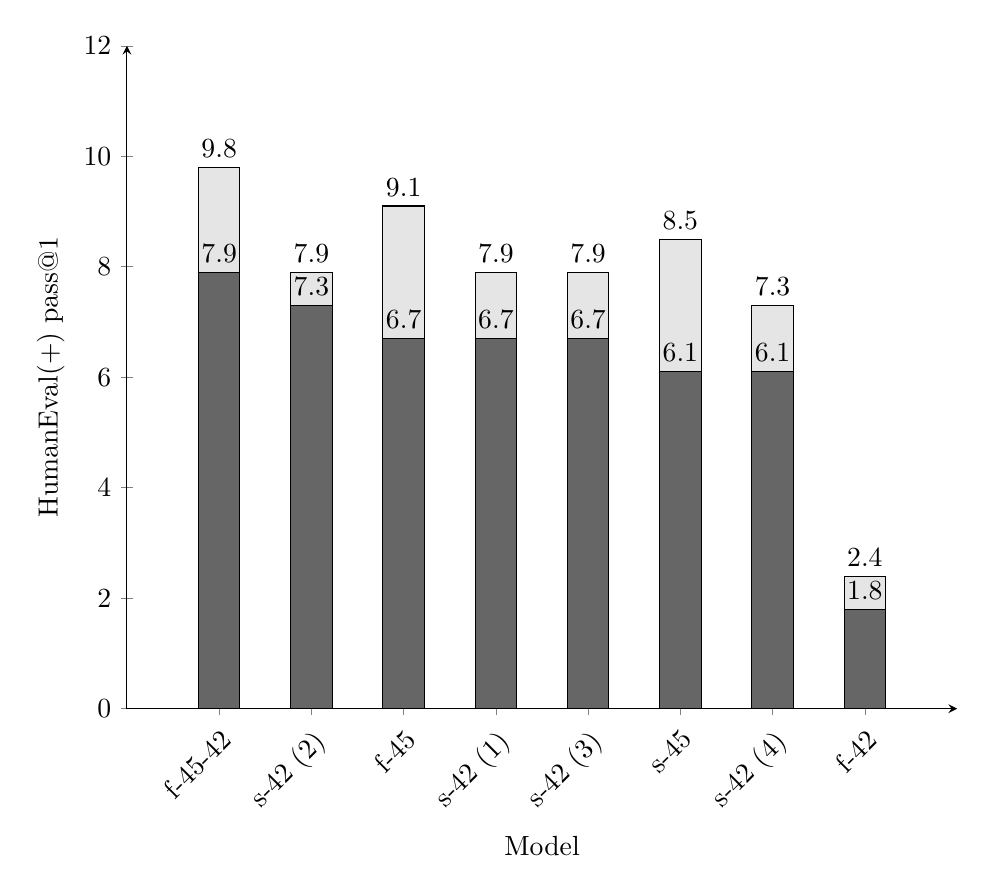
\begin{tikzpicture}
        \begin{axis}[
            ybar,
            xtick={0,1,2,3,4,5,6,7}, % Set xticks to match data points
            xticklabels={f-45-42, s-42 (2), f-45, s-42 (1), s-42 (3), s-45, s-42 (4), f-42},
            ylabel={HumanEval(+) pass@1},
            xlabel={Model},
            ymin=0,
            ymax=12,
            bar width=15pt,
            nodes near coords,
            width=\textwidth,
            height=10cm,
            enlarge x limits=0.15,
            x tick label style={rotate=45, anchor=north east},
            axis x line=bottom,
            axis y line=left,
            every axis plot/.append style={bar shift=0pt},
            xmin=-1,
            xmax=8
        ]
    
        % HumanEval
        \addplot[ybar,fill=black!10] plot coordinates {(0, 9.8) (1, 7.9) (2, 9.1) (3, 7.9) (4, 7.9) (5, 8.5) (6, 7.3) (7, 2.4)};
    
        % HumanEval+
        \addplot[ybar,fill=black!60] plot coordinates {(0, 7.9) (1, 7.3) (2, 6.7) (3, 6.7) (4, 6.7) (5, 6.1) (6, 6.1) (7, 1.8)};
    
        \end{axis}
    \end{tikzpicture}
    \caption{Pass@1 rates for HumanEval (light bar) and HumanEval+ (dark bar) with TinyLlama-v1.0 fine-tuned on various dataset samples. f and s refer to stratified and fixed sampling, the number after the dash to the seed used for sampling. The number in the brackets refers to the epoch count, if it was trained for multiple (on the same dataset). f-42 did not use the start and end tokens. f-45-42 was trained on the fixed-45 sample, then the fixed-42 sample (with tokens).}
    \label{fig:pretrainone}
\end{figure}

The second round of testing was to see if altering the \ac{lora} rank and alpha values could improve performance.
Starting here, fine-tuning was done with stratified sampled chunks with seeds counting up from 0.
In this case, where only one episode was trained, the data was seeded with 0.
The combinations tested were the original rank 64 alpha 16 as well as two adaptations for the double and half rule: rank 64 alpha 32 and rank 8 alpha 16.
As can be seen in figure \ref{fig:pretraintwo}, the other variants performed worse than the original.

\begin{figure}[H]
    \centering
    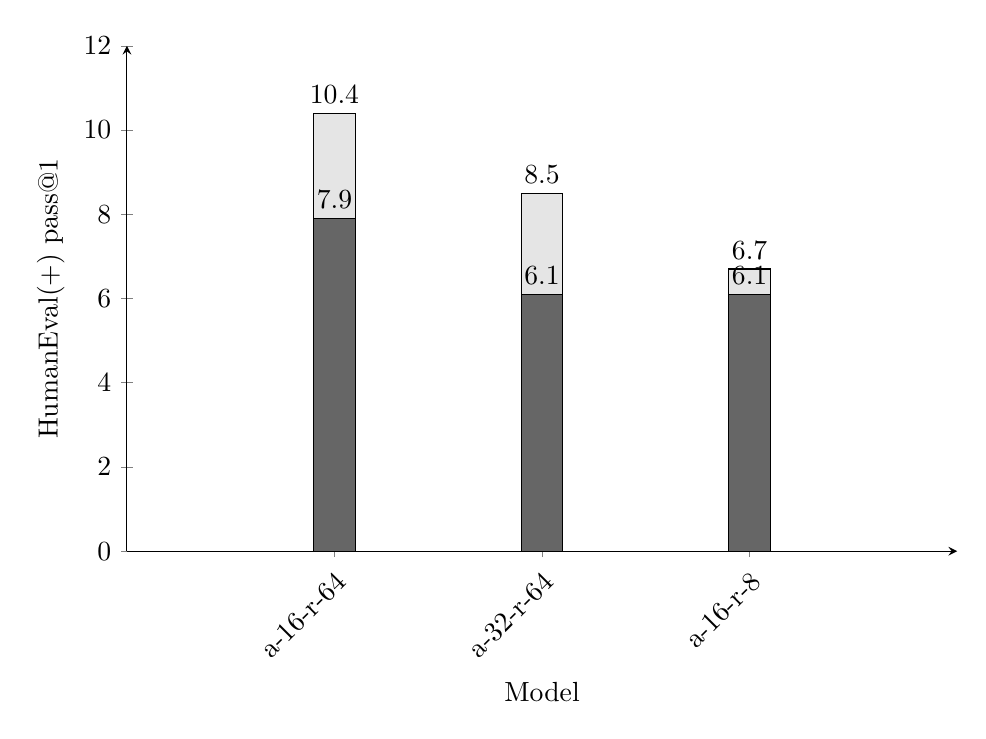
\begin{tikzpicture}
        \begin{axis}[
            ybar,
            xtick={0,1,2}, % Set xticks to match data points
            xticklabels={a-16-r-64, a-32-r-64, a-16-r-8}, % Corresponding labels
            ylabel={HumanEval(+) pass@1},
            xlabel={Model},
            ymin=0,
            ymax=12,
            bar width=15pt, % Adjust bar width
            nodes near coords,
            width=\textwidth, % Adjust width
            height=8cm, % Adjust height
            enlarge x limits=0.15, % Adjust x limits for spacing
            x tick label style={rotate=45, anchor=north east}, % Rotate labels if needed
            axis x line=bottom, % Ensure x-axis is drawn at the bottom
            axis y line=left, % Ensure y-axis is drawn on the left
            every axis plot/.append style={bar shift=0pt}, % Remove any default bar shift
            xmin=-1,
            xmax=3
        ]

        % HumanEval
        \addplot[ybar,fill=black!10] plot coordinates {(2, 6.7) (0, 10.4) (1, 8.5)};

        % HumanEval+
        \addplot[ybar,fill=black!60] plot coordinates {(2, 6.1) (0, 7.9) (1, 6.1)};

        \end{axis}
    \end{tikzpicture}
    \caption{Pass@1 rates for HumanEval (light bar) and HumanEval+ (dark bar) with TinyLlama-v1.0 fine-tuned on the first data chunk. a and r refer to alpha and rank, the number after the dash to their value.}
    \label{fig:pretraintwo}
\end{figure}

The final step of pre-testing was the experimentation for swapping out datasets mid-training.
The third iteration is not shown as it was visibly faulty when starting training and never finished an epoch, while the fourth iteration led into final training, the results of which are presented in the upcoming sections.
As seen in \ref{fig:pretrainthree}, the results are still concentrated around the same percentage values, while not necessarily improving with multiple epochs.
Also notable is that the HumanEval and HumanEval+ results improved over the results from the same configuration in figure \ref{fig:pretraintwo} (a-16-r-64 and v1 (1) are trained identically).
This is due to the temperature of the generator pipeline, resulting in slight variations in score when generating.
The temperature is taken from the model, in this case 1.0.
This is a discrepancy that was not noticed until final training began.
As there are no major outliers in evaluation so far, it can be assumed that this had no major impact on the results for final training.

Because results did not improve with training, and because using seeded sampling could still cause overlap in data trained on, leading to unpredictable training data and results, the data was split into 100 stratified chunks that were saved locally.
These chunks contain no overlap, instead being an even division of the data.
This, along with the other changes of the fourth iteration, were hoped to result in better performance when training for more epochs.

\begin{figure}[H]
    \centering
    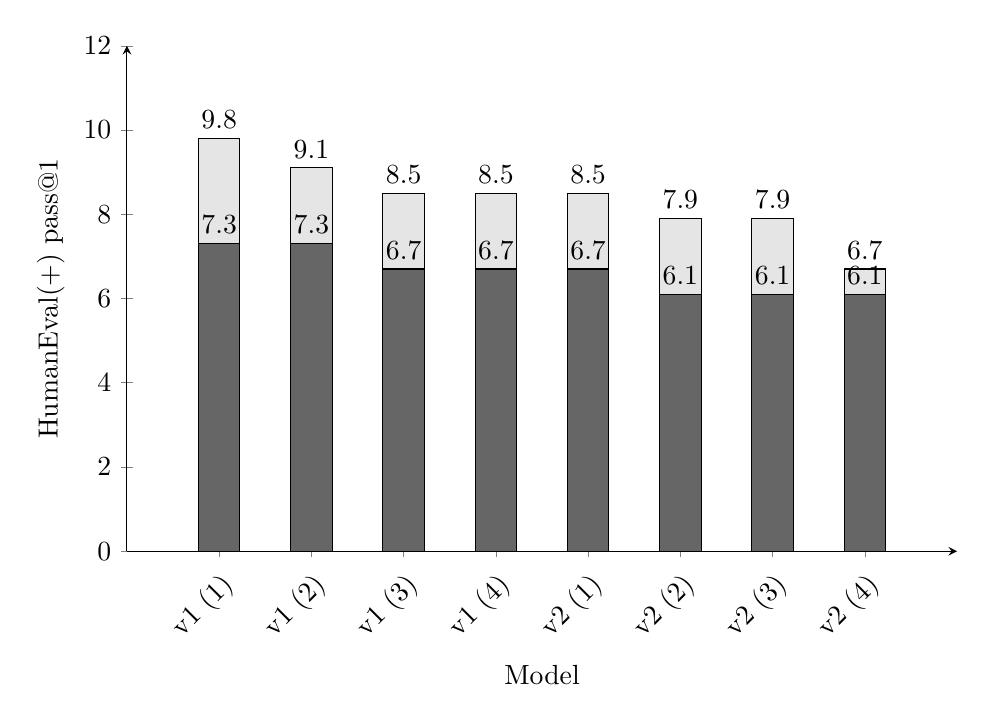
\begin{tikzpicture}
        \begin{axis}[
            ybar,
            xtick={0,1,2,3,4,5,6,7},
            xticklabels={v1 (1), v1 (2), v1 (3), v1 (4), v2 (1), v2 (2), v2 (3), v2 (4)},
            ylabel={HumanEval(+) pass@1},
            xlabel={Model},
            ymin=0,
            ymax=12,
            bar width=15pt,
            nodes near coords,
            width=\textwidth,
            height=8cm,
            enlarge x limits=0.15,
            x tick label style={rotate=45, anchor=north east},
            axis x line=bottom,
            axis y line=left,
            every axis plot/.append style={bar shift=0pt},
            xmin=-1,
            xmax=8
        ]

        % HumanEval
        \addplot[ybar,fill=black!10] plot coordinates {(7, 6.7) (5, 7.9) (1, 9.1)(2, 8.5) (0,9.8) (6,7.9) (3, 8.5) (4,8.5)};

        % HumanEval+
        \addplot[ybar,fill=black!60] plot coordinates {(7, 6.1) (5, 6.1) (1, 7.3)(2, 6.7) (0,7.3) (6,6.1) (3,6.7) (4,6.7)};

        \end{axis}
    \end{tikzpicture}
    \caption{Pass@1 rates for HumanEval (light bar) and HumanEval+ (dark bar) with TinyLlama-v1.0 fine-tuned on various dataset samples. v1 and v2 refer to the first and second iteration described in section \ref{sec:pretrain}, the bracketed number to the epoch count. As seeds count up from 0, epoch 4 is trained on data from seeds 0, 1, 2 and 3.}
    \label{fig:pretrainthree}
\end{figure}


\section{Results on Code Synthesis Metrics}
\label{sec:metricresults}

This section will show the results on all chosen metrics individually, with an overview of all results in section \ref{sec:resoverview}.
In this section, the TinyLlama models will be abbreviated as TL and the TinyFuncCoder models as TFC.
Reformatted prompts (R) indicate prompts that have been altered to fit TinyFuncCoder's data scheme from training, namely <func>, the language as a comment, the docstring, then the head and parameters.
Any extra information such as imports or class structures is put before the function tag.

\subsection{Results Overview}
\label{sec:resoverview}
This section will provide an overview of the main results, compiling all individual metrics into a single table.
For metrics that are divided into multiple categories, like DS-1000, the average of all categories is given.
Each metric is discussed individually in the upcoming sections.

\begin{table}[h]
    \centering
    \small
    \caption{Pass@1 comparison between the TinyFuncCoder series and TinyLlama series on all metrics. TinyLlama values were calculated alongside TinyFunc-
    Coder. (R) indicates a reformatted prompt for evaluation. For the multi-value metrics, DS-1000, MultiPL-E and HumanEvalPack, the average was taken. HumanEvalPack was not included as it is equivalent to HumanEval, as discussed in section \ref{sec:humanevalpackres}.}
    \begin{tabular}{l|rrrrrr}
        \hline
        Model & Human & MBPP(+) & MultiPL-E & MultiPL-E & DS-1000 & Avg. \\
         & Eval(+) & & (featured) & (other) & \\
        \hline
        TL-v1.0 & 12.20 (10.98) & 0.60 (0.53) & 3.76 & 6.64 & 1.60 & 5.19 \\
        \textbf{TFC-v1.0} & \textbf{9.76 (8.54)} & \textbf{8.20 (9.26)} & \textbf{7.52} & \textbf{8.68} & \textbf{0.70} & \textbf{7.45} \\
        TL-v1.1 & 1.22 (1.22) & 2.60 (3.17) & 2.46 & 6.57 & 0.70 & 2.56 \\
        TL-v1.1\_mc & 6.70 (4.88) & 13.00 (17.20) & 5.55 & 9.08 & 1.80 & 8.32 \\
        \textbf{TFC-v1.1} & \textbf{0.00 (0.00)} & \textbf{0.00 (0.00)} & \textbf{0.00} & \textbf{0.00} & \textbf{0.00} & \textbf{0.00} \\
        \hline
        TL-v1.0 (R) & 7.93 (7.32) & 12.00 (15.08) & 4.46 & - & 0.10 & 7.82 \\
        \textbf{TFC-v1.0 (R)} & \textbf{9.76 (8.54)} & \textbf{12.80 (19.58)} & \textbf{11.07} & \textbf{-} & \textbf{1.00} & \textbf{10.46} \\
        TL-v1.1 (R) & 3.66 (3.66) & 3.00 (4.50) & 2.82 & - & 0.20 & 2.97 \\
        TL-v1.1\_mc (R) & 14.02 (12.20) & 8.20 (10.85) & 6.89 & - & 0.10 & 8.71 \\
        \textbf{TFC-v1.1 (R)} & \textbf{0.00 (0.00)} & \textbf{0.00 (0.26)} & \textbf{0.00} & \textbf{-} & \textbf{0.00} & \textbf{0.04} \\
        \hline
    \end{tabular}
    \label{tab:resoverview}
\end{table}

As can be seen in table \ref{tab:resoverview}, TinyFuncCoder-v1.0 improves over TinyLlama-v1.0 in some metrics while worsening in others, and TinyFuncCoder-v1.1 is broadly unsuccessful in generating correct solutions.
The TinyFuncCoder-v1.0 average sits above TinyLlama-v1.0, and even above TinyLlama-v1.1\_math\_code when taking the reformatted prompt into consideration.
However, this is likely inflated due to PHP and Go, as will be discussed in section \ref{sec:multipleres}.


\subsection{Results on HumanEval(+)}
\label{sec:humanevalres}

This section will showcase TinyFuncCoder performance on HumanEval.
Because this is the most well-known and commonly used evaluation metric for code synthesis models, it was also used for evaluating TinyFuncCoder-v1.0 after each training epoch to see if model improvements could be monitored.
The results to this are shown in figure \ref{fig:humaneval}.

\begin{figure}[!h]
    \centering
    \begin{tikzpicture}
        \begin{axis}[
            xlabel={Chunk (Epoch)},
            ylabel={pass@1},
            ymin=6,
            ymax=12,
            xmin=0,
            xmax=37,
            xtick distance=2,
            ytick distance=1,
            grid=major,
            width=\textwidth,
            height=\textwidth/2,
            legend pos=south east,
            every axis plot/.append style={thick, line width=3pt},
        ]
        
        \addlegendimage{black, thick, line width=2pt}
        \addlegendentry{TinyLlama-v1.0}
        
        \addlegendimage{blue, thick, mark=square, line width=3pt}
        \addlegendentry{HumanEval}

        \addlegendimage{red, thick, mark=square, line width=3pt}
        \addlegendentry{HumanEval+}

        \addplot[
            color=black,
            thick,
            domain=0:37,
            line width=2pt
        ]
        {9.15};

        %%%%%%%%%%%%%%%%%%%%%%%%%%%%%%%%%%%%%%%%%%%%%%%%%%%%%%%%%
        \addplot[color=blue!30,mark=square]
        coordinates {
            (10,9.8)
            
            (12,9.1)
            
            (14,9.1) (15,10.4) (16,10.4) (17,11) (18,9.8)
        };
        %%%%%%%%%%%%%%%%%%%%%%%%%%%%%%%%%%%%%%%%%%%%%%%%%%%%%%%%%
        \addplot[color=red!30,mark=square]
        coordinates {
            (10,7.9)
            
            (12,7.9)
            
            (14,7.3) (15,9.1) (16,8.5) (17,9.8) (18,8.5)
        };
        %%%%%%%%%%%%%%%%%%%%%%%%%%%%%%%%%%%%%%%%%%%%%%%%%%%%%%%%%
        \addplot[color=blue!100,mark=square]
        coordinates {
            (0,8.5) (1,9.1) (2,8.5)
        
            (5,9.8) (6,10.4) (7,10.4) (8,10.4)
            
            (10,10.4)
            
            (12,9.1)
            
            (14,9.8) (15,10.4) (16,10.4) (17,9.8) (18,9.8)
            
            (21,9.1)
            
            (24,11)
            
            (26,9.1)
            
            (29,10.4) (30,10.4) (31,9.8) (32,9.8) (33,9.8)
            
            (35,9.8)
            
            (37,9.8)
        };
        %%%%%%%%%%%%%%%%%%%%%%%%%%%%%%%%%%%%%%%%%%%%%%%%%%%%%%%%%
        \addplot[color=red!100,mark=square]
        coordinates {
            (0,7.3) (1,8.5) (2,7.3)
            
            (5,8.5) (6,9.1) (7,9.1) (8,9.1)
            
            (10,9.1)
            
            (12,8.5)
            
            (14,7.9) (15,9.1) (16,8.5) (17,9.1) (18,8.5)
            
            (21,7.9)
            
            (24,9.8)
            
            (26,7.9)
            
            (29,9.1) (30,8.5) (31,9.1) (32,8.5) (33,8.5)
            
            (35,8.5)
            
            (37,8.5)
        };
        %%%%%%%%%%%%%%%%%%%%%%%%%%%%%%%%%%%%%%%%%%%%%%%%%%%%%%%%%

        \begin{comment}
            % experimental vals
            %%%%%%%%%%%%%%%%%%%%%%%%%%%%%%%%%%%%%%%%%%%%%%%%%%%%%%%%%
            \addplot[color=blue!30,mark=square]
            coordinates {
                (10,9.8)
                
                (12,9.1)
                
                (14,9.1) (15,10.4) (16,10.4) (17,11) (18,9.8)
            };
            %%%%%%%%%%%%%%%%%%%%%%%%%%%%%%%%%%%%%%%%%%%%%%%%%%%%%%%%%
            \addplot[color=red!30,mark=square]
            coordinates {
                (10,7.9)
                
                (12,7.9)
                
                (14,7.3) (15,9.1) (16,8.5) (17,9.8) (18,8.5)
            };
            %%%%%%%%%%%%%%%%%%%%%%%%%%%%%%%%%%%%%%%%%%%%%%%%%%%%%%%%%
            \addplot[color=blue!100,mark=square]
            coordinates {
                (0,9.8) (1,9.8) (2,7.3)
            
                (5,9.1) (6,9.8) (7,9.8) (8,8.5)
                
                (10,7.9)
                
                (12,9.1)
                
                (14,9.1) (15,8.5) (16,9.8) (17,9.1) (18,11)
                
                (21,8.5)
                
                (24,10.4)
                
                (26,7.9)
                
                (29,9.1) (30,10.4) (31,9.8) (32,9.1) (33,9.8)
                
                (35,9.8)
                
                (37,8.5)
            };
            %%%%%%%%%%%%%%%%%%%%%%%%%%%%%%%%%%%%%%%%%%%%%%%%%%%%%%%%%
            \addplot[color=red!100,mark=square]
            coordinates {
                (0,8.5) (1,8.5) (2,6.7)
                
                (5,8.5) (6,9.1) (7,8.5) (8,7.9)
                
                (10,6.7)
                
                (12,8.5)
                
                (14,8.5) (15,7.9) (16,7.9) (17,8.5) (18,9.8)
                
                (21,7.3)
                
                (24,8.5)
                
                (26,7.3)
                
                (29,7.9) (30,8.5) (31,8.5) (32,8.5) (33,9.8)
                
                (35,9.1)
                
                (37,7.3)
            };
            %%%%%%%%%%%%%%%%%%%%%%%%%%%%%%%%%%%%%%%%%%%%%%%%%%%%%%%%%
        \end{comment}

        \end{axis}
    \end{tikzpicture}
    \caption{Pass@1 on HumanEval and HumanEval+ for each epoch TinyLlama-v1.0 was fine-tuned. Chunks without a point have been skipped due to memory crashes. The black line shows TinyLlama's performance on HumanEval without any fine-tuning.
    The lighter lines are performance of the checkpoints trained from the wrong starting point, as mentioned in section \ref{sec:finaltrain}. If the blue line goes below the black, the model's performance has worsened from fine-tuning. Model performance was evaluated with the EvalPlus implementation, not the Bigcode Evaluation Harness implementation.}
    \label{fig:humaneval}
\end{figure}

While model performance on HumanEval(+) is unstable, the tendancy does trend upwards. The earliest epochs perform worse than the base model, but improve to be equal to or better than TinyLlama-v1.0 after just a few epochs.
It can also be noted that HumanEval and HumanEval+ performance is not directly linked.
For example, at chunk 17 HumanEval performance drops, but HumanEval+ performance rises.
This makes sense -- HumanEval+ expands the test suite for HumanEval.
A generation that HumanEval judged as correct could be rejected by HumanEval+, improving the former while keeping the latter the same.
Conversely, a task that was already correct according to HumanEval could be improved to also be approved by HumanEval+, keeping the former the same while improving the latter.
Also of note is that the training from a wrong starting checkpoint, shown in the lighter lines, match the best epoch of evaluation, 24.
Another important factor is the temperature used for generating.
For all results in this section, it is set to 0.2.
While this relatively low, it will still lead to some variance when generating answers.
Even when prompting an identical model multiple times with the same question, results may differ.
Performance can only improve or worsen in steps of $1/164$, or about 0.6\%, so correctly or incorrectly generating one or two questions due to variations caused by the temperature can already shift pass@1 by a percentage point.
Also interesting is that there are two sections where performance stays broadly consistens -- chunks six to ten and chunks 31 to 37.


\begin{table}[!h]
    \centering
    \caption{HumanEval(+) pass@1 comparison between the TinyFuncCoder series and contemporary models. Values taken from the EvalPlus leaderboard. Models without a size are closed-source. TinyLlama values were calculated alongside TinyFuncCoder. (R) indicates a reformatted prompt for evaluation.}
    \begin{tabular}{l|rr|r}
        \hline
        Model & HumanEval & HumanEval+ & Size \\
        \hline
        GPT-4-Turbo (April 2024) & 90.20 & 86.60 & - \\ claude-3-opus (Mar 2024) & 82.90 & 77.40 & - \\
        \hline
        DeepSeek-Coder-V2-Instruct & 88.40 & 82.30 & 236 B \\
        OpenCodeInterpreter-DS-33B & 79.30 & 73.80 & 33 B \\
        WizardCoder-33B-V1.1 & 79.90 & 73.20 & 33 B \\
        Magicoder-S-DS-6.7B & 76.80 & 71.30 & 6.7 B \\
        DeepSeek-Coder-1.3B-Base & 28.70 & 25.60 & 1.3 B \\
        \hline
        TL-v1.0 & 12.20 & 10.98 & 1.1 B \\
        \textbf{TFC-v1.0} & \textbf{9.76} & \textbf{8.54} & \textbf{1.1 B} \\
        TL-v1.1 & 1.22 & 1.22 & 1.1 B \\
        TL-v1.1\_mc & 6.70 & 4.88 & 1.1 B \\
        \textbf{TFC-v1.1 (R)} & \textbf{0.00} & \textbf{0.00} & \textbf{1.1 B} \\
        \hline
        TL-v1.0 (R) & 7.93 & 7.32 & 1.1 B \\
        \textbf{TFC-v1.0 (R)} & \textbf{9.76} & \textbf{8.54} & \textbf{1.1 B} \\
        TL-v1.1 (R) & 3.66 & 3.66 & 1.1 B \\
        TL-v1.1\_mc (R) & 14.02 & 12.20 & 1.1 B \\
        \textbf{TFC-v1.1 (R)} & \textbf{0.00} & \textbf{0.00} & \textbf{1.1 B} \\
        \hline
    \end{tabular}
    \label{tab:humaneval}
\end{table}

Table \ref{tab:humaneval} shows the pass@1 rates of TinyFuncCoder in comparison to other models presented in this thesis.
The rates of the other models come from the EvalPlus leaderboard\footnote{\url{https://evalplus.github.io/leaderboard.html} (last visited on 2024-10-31)}.
A few things become quickly apparent: pass@k rates seem to be proportional to model size, with bigger models having massively better results than smaller models.
This trend continues to the closed-source models as well -- GPT4 has been estimated to have 1.8 T parameters by multiple experts\footnote{\url{https://www.youtube.com/watch?v=K5iDUZPx60E&t=2989s} (last visited on 2024-10-31),
\\\url{https://www.semianalysis.com/p/gpt-4-architecture-infrastructure} (last visited on 2024-10-31),
\\\url{https://preview.redd.it/d-same-param-count-for-gpt4-from-nvidia-gtc24-as-the-leak-v0-vyzfx2sel5pc1.png?width=1764&format=png&auto=webp&s=58b33f4fe36915163f74ff9dea329af58be3ce51} (last visited on 2024-10-31),
\\\url{https://x.com/soumithchintala/status/1671267150101721090} (last visited on 2024-10-31)}.
As for the TinyLlama and the TinyFuncCoder series, the following is of note:
First, TinyFuncCoder-v1.0 is worse than its respective base model, and TinyFuncCoder-v1.1 has a pass rate of zero.
TinyLlama-v1.0 actually performs better than listed in their paper, scoring 12.2 rather than the 9.15 listed.
TinyFuncCoder-v1.0 does improve on the 9.15 listed, scoring 9.76 which is equivalent to one extra problem solved correctly, but not on the newly calculated 12.2.
It is also notable that reformatting the prompt to the TinyFuncCoder template has inconsistent effects among the models, with some improving (even drastically, like TinyLlama-v1.1\_math\_code, which more than doubles its pass@1), some becoming worse (like TinyLlama-v1.0), and TinyFuncCoder-v1.0 not being affected at all.
Surprisingly, even TinyLlama-v1.1 can generate some correct code without being explicitly trained on code, which makes the fact that TinyFuncCoder-v1.1 cannot even more surprising.
Overall, TinyFuncCoder does not improve on TinyLlama.
Further, DeepSeekCoder-1.3B-Base achieves between double and triple the performance with only an extra 200 M parameters.


\subsection{Results on MBPP(+)}
\label{sec:mbppres}

On MBPP(+), overall results -- shown in table \ref{tab:mbpp} -- are very similar to HumanEval, with increasing model size broadly translating to better performance.
DeepSeek-Coder-1.3B-Base also outperforms the TinyLlama and TinyFuncCoder models by a wide margin and TinyFuncCoder-v1.1 sits at zero again.
There are some unexpected results for this metric, starting with TinyLlama-v1.0, which performs surprisingly bad, even worse than v1.1 without code training.
Results were generated multiple times with unchanged performance.
Using the reformatted prompt, TinyLlama-v1.0 suddenly performs normally.
It is unclear what causes this behaviour.
Notably, TinyFuncCoder-v1.0 outperforms TinyLlama-v1.0 with a reformatted prompt, and is even comparable to TinyLlama-v1.1\_math\_code.
Next, performance on MBPP+ improves for the models evaluated for this thesis (TinyLlama and TinyFuncCoder), but worsens on all others.
This may be related to the fact that MBPP+ has 378 questions, while MBPP has 500.
$378/500$ gives a ratio of around 1.32 which is broadly consistent with the difference in MBPP to MBPP+ scores of the manually evaluated models (avg. 1.27, med. 1.29), but does not explain why the other models do not also experience this improvement.
MBPP+ also marks the only time where TinyFuncCoder-v1.1 generates a correct solution to any question in any metric.
Because of this, all discussions of TinyFuncCoders performance in upcoming chapters will focus on v1.0.
In summary, the best TinyFuncCoder results improve over the best TinyLlama results on MBPP and MBPP+.

\begin{table}[!h]
    \centering
    \caption{MBPP(+) pass@1 comparison between the TinyFuncCoder series and contemporary models. Values taken from the EvalPlus leaderboard. Models without a size are closed-source. TinyLlama values were calculated alongside TinyFuncCoder. (R) indicates a reformatted prompt for evaluation.}
    \begin{tabular}{l|rr|r}
        \hline
        Model & MBPP & MBPP+ & Size \\
        \hline
        claude-3-opus (Mar 2024) & 89.4 & 73.3 & - \\
        GPT-4-Turbo (Nov 2023) & 85.7 & 73.3 & - \\
        \hline
        DeepSeek-Coder-V2-Instruct & 89.40 & 75.10 & 236 B \\
        WizardCoder-Python-34B-V1.0 & 75.10 & 63.20 & 34 B \\
        OpenCodeInterpreter-DS-33B & 80.2 & 68.5 & 33 B \\
        Magicoder-S-DS-6.7B & 79.40 & 69.00 & 6.7 B \\
        DeepSeek-Coder-1.3B-Base & 56.9 & 47.9 & 1.3 B \\
        \hline
        TL-v1.0 & 0.60 & 0.53 & 1.1 B \\
        \textbf{TFC-v1.0} & \textbf{8.20} & \textbf{9.26} & \textbf{1.1 B} \\
        TL-v1.1 & 2.60 & 3.17 & 1.1 B \\
        TL-v1.1\_mc & 13.00 & 17.20 & 1.1 B \\
        \textbf{TFC-v1.1} & \textbf{0.00} & \textbf{0.00} & \textbf{1.1 B} \\
        \hline
        TL-v1.0 (R) & 12.00 & 15.08 & 1.1 B \\
        \textbf{TFC-v1.0 (R)} & \textbf{12.80} & \textbf{19.58} & \textbf{1.1 B} \\
        TL-v1.1 (R) & 3.00 & 4.50 & 1.1 B \\
        TL-v1.1\_mc (R) & 8.20 & 10.85 & 1.1 B \\
        \textbf{TFC-v1.1 (R)} & \textbf{0.00} & \textbf{0.26} & \textbf{1.1 B} \\
        \hline
    \end{tabular}
    \label{tab:mbpp}
\end{table}


\subsection{Results on MultiPL-E}
\label{sec:multipleres}

\subsubsection{Featured Languages}
\label{sec:multiplefeatured}
On MultiPL-E, a pass@1 score is calculated for each language individually.
MultiPL-E consists of more languages than those listed, but only languages which TinyFuncCoder was trained on are evaluated in this section.
Results can be seen in table \ref{tab:multiplefeat}.
Of the models mentioned in this paper, only WizardCoder and Magicoder provided results on this metric, and not for all languages.
Languages without a pass rate were marked with a dash.
On MultiPL-E, TinyFuncCoder broadly matches or outperforms TinyLlama-v1.0 and even TinyLlama-v1.1\_math\_code, especially on C++, C\# and Java.
It is also the only model to generate a correct solution for a Shell problem.

\begin{table}[!h]
    \centering
    \caption{MultiPL-E pass@1 comparison between the TinyFuncCoder series and contemporary models. Values for Magicoder and WizardCoder from \cite{Wei.2024}. TinyLlama values were calculated alongside TinyFuncCoder. (R) indicates a reformatted prompt for evaluation.}
    \scriptsize
    \begin{tabular}{l|rrrrrrrrr|r}
        \hline
        Model & C++ & C\# & Java & JavaScript & PHP & Ruby & Shell & TypeScript & Avg. & Size \\
        \hline
        WizardCoder-CL & 47.20 & - & 44.90 & 55.30 & 47.20 & - & - & - & 48.65 & 34 B \\
        Magicoder$\mathcal{S}$-CL & 44.40 & - & 42.90 & 57.50 & 47.60 & - & - & - & 48.10 & 7 B \\
        \hline
        TL-v1.0 & 6.83 & 3.80 & 6.96 & 0.62 & 6.21 & 6.21 & 0.00 & 1.89 & 3.76 & 1.1 B \\
        \textbf{TFC-v1.0} & \textbf{9.94} & \textbf{3.40} & \textbf{7.59} & \textbf{6.21} & \textbf{21.12} & \textbf{5.60} & \textbf{0.63} & \textbf{5.66} & \textbf{7.52} & \textbf{1.1 B} \\
        TL-v1.1 & 4.35 & 3.16 & 4.43 & 1.86 & 3.73 & 1.24 & 0.00 & 1.26 & 2.46 & 1.1 B \\
        TL-v1.1\_mc & 6.21 & 4.43 & 4.43 & 9.94 & 9.94 & 1.24 & 0.00 & 8.18 & 5.55 & 1.1 B \\
        \textbf{TFC-v1.1} & \textbf{0.00} & \textbf{0.00} & \textbf{0.00} & \textbf{0.00} & \textbf{0.00} & \textbf{0.00} & \textbf{0.00} & \textbf{0.00} & \textbf{0.00} & \textbf{1.1 B} \\
        \hline
        TL-v1.0 (R) & 8.07 & 5.70 & 7.59 & 0.62 & 7.45 & 4.97 & 0.00 & 1.26 & 4.46 & 1.1 B \\
        \textbf{TFC-v1.0 (R)} & \textbf{9.94} & \textbf{6.33} & \textbf{7.59} & \textbf{9.32} & \textbf{45.34} & \textbf{5.60} & \textbf{0.00} & \textbf{4.40} & \textbf{11.07} & \textbf{1.1 B} \\
        TL-v1.1 (R) & 4.35 & 2.53 & 2.00 & 4.35 & 3.73 & 1.86 & 0.00 & 3.77 & 2.82 & 1.1 B \\
        TL-v1.1\_mc (R) & 6.21 & 6.96 & 8.86 & 8.07 & 8.70 & 4.35 & 0.00 & 11.95 & 6.89 & 1.1 B \\
        \textbf{TFC-v1.1 (R)} & \textbf{0.00} & \textbf{0.00} & \textbf{0.00} & \textbf{0.00} & \textbf{0.00} & \textbf{0.00} & \textbf{0.00} & \textbf{0.00} & \textbf{0.00} & \textbf{1.1 B} \\
        \hline
    \end{tabular}
    \label{tab:multiplefeat}
\end{table}

Of note is that the evaluation for PHP was troublesome. It often took much longer than the other languages and caused the WSL integration to crash during evaluation.
It generated incredibly good scores (as high as 99) because of an incorrectly reformatted prompt (removing \texttt{<?php} at the start), and PHP results on TinyFuncCoder still seem unreasonably high when compared to the other languages and models.
This raises concerns -- if the result was correct despite an important piece of syntax missing, the evaluation for at least PHP can be seen as unreliable, and it being an outlier seems to confirm this.
Similar issues did not occur for other languages.
No correlation between the performance of the regular and reformatted prompt and the extent of prompt reformatting seems to exist.
C++, C\# and Java had extensive reformatting while JavaScript, PHP, Ruby, Shell and TypeScript remained relatively the same.
Among both groups, models perform broadly similar, with occasional outliers in both.
Overall, MultiPL-E shows the success of training TinyFuncCoder for multiple languages, as it broadly improves on TinyLlama.

With MultiPL-E expanding the testing suite to an additional eight languages, the only language on which TinyFuncCoder was trained that has not been evaluated is C.
Unfortunately, none of the other metrics evaluate C either, leaving it completely untested.
Interesting to note is that MultiPL-E, while adapting the original 164 HumanEval questions into multiple languages, does not have the same amount of problems for each language.
The number of questions fluctuates between 164 and as low as 154 for Go, presumably due to language-specific questions falling away.


\subsubsection{Other Languages}
\label{sec:multipleother}
This section evaluates all MultiPL-E languages which TinyFuncCoder was not fine-tuned on at all.
As the main focus of TinyFuncCoder are the ten languages it was trained on, these results can be seen as secondary.
Poor performance on these languages is much less relevant than on the featured languages.
On the flipside, good performance on these languages could showcase good transfer learning from TinyFuncCoder, especially if it performs better than TinyLlama, which was trained on these languages.
Because of the lesser importance of these tests, generations will only be produced with the basic template.
No adjusted template for TinyFuncCoder was created.
Unfortunately, evaluation for Clojure, Dart, Elixir, Haskell and ML was not possible.
Code for these languages has been generated and will be uploaded to the repository, but could not be evaluated because the respective metrics do not exist yet within the Bigcode framework.
Results are shown in table \ref{tab:multipleother}.

\begin{table}[!h]
    \centering
    \small
    \caption{MultiPL-E pass@1 comparison between the TinyFuncCoder series and TinyLlama series on languages TinyFuncCoder was not trained on.}
    \begin{tabular}{l|rrrrrrrr|r}
        \hline
        Model & Clojure & D & Dart & Elixir & Go & Haskell & Julia & Lua & Size \\
        \hline
        TL-v1.0 & - & 1.28 & - & - & 31.82 & - & 3.77 & 2.48 & 1.1 B\\
        \textbf{TFC-v1.0} & \textbf{-} & \textbf{4.49} & \textbf{-} & \textbf{-} & \textbf{58.44} & \textbf{-} & \textbf{0.00} & \textbf{0.62} & \textbf{1.1 B} \\
        TL-v1.1 & - & 2.56 & - & - & 49.35 & - & 0.63 & 1.86 & 1.1 B \\
        TL-v1.1-mc & - & 5.13 & - & - & 48.70 & - & 6.92 & 5.59 & 1.1 B \\
        \textbf{TFC-v1.1} & \textbf{-} & \textbf{0.00} & \textbf{-} & \textbf{-} & \textbf{0.00} & \textbf{-} & \textbf{0.00} & \textbf{0.00} & \textbf{1.1 B} \\
        &&&&&&&&\\
        \hline
        Model & ML & Perl & R & Racket & Rust & Scala & Swift & Avg. & Size \\
        \hline
        WizardCoder-CL & - & - & - & - & 46.20 & - & 44.30 & 45.25 & 34 B \\
        Magicoder$\mathcal{S}$-CL & - & - & - & - & 40.30 & - & 44.10 & 42.20 & 7 B \\
        \hline
        TL-v1.0 & - & 1.86 & 4.35 & 3.10 & 6.41 & 7.50 & 3.80 & 6.64 & 1.1 B \\
        \textbf{TFC-v1.0} & \textbf{-} & \textbf{1.24} & \textbf{4.35} & \textbf{2.48} & \textbf{5.77} & \textbf{5.00} & \textbf{4.43} & \textbf{8.68} & \textbf{1.1 B} \\
        TL-v1.1 & - & 2.48 & 1.24 & 0.00 & 1.92 & 3.13 & 2.53 & 6.57 & 1.1 B \\
        TL-v1.1-mc & - & 2.48 & 5.59 & 2.48 & 2.56 & 5.63 & 5.70 & 9.08 & 1.1 B \\
        \textbf{TFC-v1.1} & \textbf{-} & \textbf{0.00} & \textbf{0.00} & \textbf{0.00} & \textbf{0.00} & \textbf{0.00} & \textbf{0.00} & \textbf{0.00} & \textbf{1.1 B} \\
        \hline
    \end{tabular}
    \label{tab:multipleother}
\end{table}

While it can be seen that TinyFuncCoder improves on three languages when compared to TinyLlama-v1.0, namely D, Go and Swift, it does perform worse on all others, but does not change for R.
Especially Julia and Lua experience a large performance drop.
The only language where it is the best among all models is Go, where all models have a suspiciously high pass rate.
This could imply that Go, similarly to PHP before, might accept false positive solutions.
The fact that it improves on D and Swift does strengthen the hypothesis that the model learns deeper coding knowledge that can be applied even to unseen languages \cite{Wei.2024}, especially considering the lack of an adapted prompt template for these problems.
Reformatting the prompts would likely improve performance even further on these languages.


\subsection{Results on HumanEvalPack}
\label{sec:humanevalpackres}

HumanEvalPack, unfortunately, was completely unreliable as a metric, with all other languages than Python resulting in a pass@1 of zero as shown in table \ref{tab:humevpack}.
As this metric was evaluated identically to the other metrics, with the BigCoder Evaluation Harness' built-in pipeline, this seems to be an issue inherent to the metric, and not caused by any work of this thesis.
Unfortunately, the papers of the other models presented in this thesis do not use this metric.
Had other models used it, it would have been more clear if it is a viable metric or not.
HumanEvalPack is also the only metric that cannot be run in a Docker container because it requires allowing remote code.
This would usually be done with the parameter \texttt{--trust\_remote\_code}, but HumanEvalPack gives an error message requesting that \texttt{--trust\_remote\_code=True} is used.
However, when calling with \texttt{True}, a warning message is given that the boolean value is explicitly set and will be ignored, causing the program to stop due to lacking permissions.
To evaluate, the argument was manually set to \texttt{True} in code, but this does not work when using a Docker container.
Due to these concerns, no reformatted prompt template was created for these tasks, as it is highly unlikely that changing the prompt would give different results.

Fortunately, all languages used in this metric have already been evaluated on MultiPL-E.
Since both are based on HumanEval, not much is lost by this metric failing, but a point of comparison would have been nice to have.
Results on HumanEvalPack-Python, which should be equivalent to base HumanEval, closely resemble the results of section \ref{sec:humanevalres}, with any deviations being explainable through generation variations due to temperature.

\begin{table}[!h]
    \centering
    \caption{HumanEvalPack pass@1 comparison between the TinyFuncCoder series and TinyLlama series. TinyLlama values were calculated alongside TinyFuncCoder. (R) indicates a reformatted prompt for evaluation.}
    \begin{tabular}{l|rrrrr|r}
        \hline
        Model & C++ & Java & JavaScript & Python & Size \\
        \hline
        TL-v1.0 & - & - & - & 12.80 & 1.1 B \\
        \textbf{TFC-v1.0} & \textbf{-} & \textbf{-} & \textbf{-} & \textbf{10.98} & \textbf{1.1 B} \\
        TL-v1.1 & - & - & - & 1.22 & 1.1 B \\
        TL-v1.1\_mc & - & - & - & 7.93 & 1.1 B \\
        \textbf{TFC-v1.1} & \textbf{-} & \textbf{-} & \textbf{-} & \textbf{0.00} & \textbf{1.1 B} \\
        \hline
    \end{tabular}
    \label{tab:humevpack}
\end{table}


\subsection{Results on DS-1000}
\label{sec:ds1000res}

For DS-1000, pass@$k$ is calculated for each of the seven Python libraries being evaluated, as well as an overall score.
The distribution of problems per library is uneven.
For the TinyLlama and TinyFuncCoder series, they only achieve results on Matplotlib.
While it is possible that this is due to an error, as the generation and evaluation pipelines are custom-written, it is also possible that the models simply do not perform well on DS-1000, a metric focused on library-specific data science problems.
With these models not performing well in general, these more specific tasks may be too challenging.
It is also noteworthy that among the models shown for comparison, Matplotlib sits about 10 to 15 points above NumPy, the next best library.
Assuming that this difference is consistent and subtracting these points from Matplotlib would place all models at zero, indicating that model performance is simply too poor to score above zero on the other libraries.
DS-1000 is also especially tricky for TinyFuncCoder, as many of the questions do not expect answers in a function format, or no function head is given to work off of.
The reformatted prompt does improve performance a bit for TinyFuncCoder, but it also vastly decreases performance of the other models.

\begin{table}[!h]
    \centering
    \caption{DS-1000 pass@1 comparison between the TinyFuncCoder series and contemporary models. Values taken from the respective papers \cite{Wei.2024,Luo.2024,Guo.2024}. Models without a size are closed-source. TinyLlama values were calculated alongside TinyFuncCoder. (R) indicates a reformatted prompt for evaluation.}
    \scriptsize
    \begin{tabular}{l|rrrrrrrr|r}
        \hline
        Model & Matplotlib & NumPy & Pandas & PyTorch & SciPy & SciKit-L. & T.Flow & Avg. & Size \\
        \hline
        WizardCoder & 55.20 & 33.60 & 16.70 & 26.20 & 24.20 & 24.90 & 26.70 & 29.20 & 34 B \\
        Magicoder$\mathcal{S}$-CL & 55.90 & 40.60 & 28.40 & 40.40 & 28.80 & 35.80 & 37.60 & 37.50 & 7 B \\
        DeepSeek-Coder-Base & 56.10 & 49.60 & 25.80 & 36.80 & 36.80 & 40.00 & 46.70 & 40.20 & 33 B \\
        \hline
        TL-v1.0 & 10.30 & 0.00 & 0.00 & 0.00 & 0.00 & 0.00 & 0.00 & 1.60 & 1.1 B \\
        \textbf{TFC-v1.0} & \textbf{4.50} & \textbf{0.00} & \textbf{0.00} & \textbf{0.00} & \textbf{0.00} & \textbf{0.00} & \textbf{0.00} & \textbf{0.70} & \textbf{1.1 B} \\
        TL-v1.1 & 2.60 & 0.00 & 0.00 & 0.00 & 0.00 & 0.00 & 0.00 & 0.70 & 1.1 B \\
        TL-v1.1\_mc & 11.60 & 0.00 & 0.00 & 0.00 & 0.00 & 0.00 & 0.00 & 1.80 & 1.1 B \\
        \textbf{TFC-v1.1} & \textbf{0.00} & \textbf{0.00} & \textbf{0.00} & \textbf{0.00} & \textbf{0.00} & \textbf{0.00} & \textbf{0.00} & \textbf{0.00} & \textbf{1.1 B} \\
        \hline
        TL-v1.0 (R) & 0.60 & 0.00 & 0.00 & 0.00 & 0.00 & 0.00 & 0.00 & 0.10 & 1.1 B \\
        \textbf{TFC-v1.0 (R)} & \textbf{6.50} & \textbf{0.00} & \textbf{0.00} & \textbf{0.00} & \textbf{0.00} & \textbf{0.00} & \textbf{0.00} & \textbf{1.00} & \textbf{1.1 B} \\
        TL-v1.1 (R) & 1.30 & 0.00 & 0.00 & 0.00 & 0.00 & 0.00 & 0.00 & 0.20 & 1.1 B \\
        TL-v1.1\_mc (R) & 0.60 & 0.00 & 0.00 & 0.00 & 0.00 & 0.00 & 0.00 & 0.10 & 1.1 B \\
        \textbf{TFC-v1.1 (R)} & \textbf{0.00} & \textbf{0.00} & \textbf{0.00} & \textbf{0.00} & \textbf{0.00} & \textbf{0.00} & \textbf{0.00} & \textbf{0.00} & \textbf{1.1 B} \\
        \hline
    \end{tabular}
    \label{tab:ds1000}
\end{table}


\section{Training and Evaluation Loss}
\label{sec:loss}

The loss for the training of the TinyFuncCoder series, seen in figures \ref{fig:v1.0loss} and \ref{fig:v1.1loss}, follows an unusual path, especially for v1.0.
Typically, it is expected for the loss to decrease during training until hitting a threshold.
In v1.0, it also often jumps back up to a much higher value, while in v1.1 such a large jump occurs only once.
It appears that the jumps occur after a crash during the training process.
For v1.0, in sections with continuous training, the loss falls relatively consistently, while resuming after one or more skipped chunks often increases the loss again.
This becomes even more apparent in v1.1, because only one chunk led to the restart of training -- chunk 21.
All other \enquote{problem chunks} were removed before training started, so training was only interrupted at chunk 21.
In v1.0, training was restarted after each problem chunk.
This worsening in loss suggests that training was not properly restarted.
It is likely that the trainer or optimizer states were not carried over during training, leading to a suboptimal training routine.
Despite this, results on the code synthesis metrics are broadly positive, as discussed in the previous sections.

\begin{figure}[!h]
    \centering
    \begin{tikzpicture}
        \begin{axis}[
            xlabel={Chunk (Epoch)},
            ylabel={Loss},
            ymin=1.325,
            ymax=1.425,
            xmin=0,
            xmax=37.5,
            xtick distance=2,
            ytick distance=.025,
            grid=major,
            width=\textwidth,
            height=\textwidth/2,
            legend pos=north east,
            every axis plot/.append style={thick, line width=2pt},
        ]
        \addlegendimage{color=blue,width=2.5pt}
        \addlegendentry{Training Loss}

        \addlegendimage{color=red,width=2.5pt}
        \addlegendentry{Evaluation Loss}

        \addplot[color=blue,width=2.5pt]
        coordinates {
            (0,1.3963) (0.5,1.3873)
            (1,1.3622) (1.5,1.3836)
            (2,1.3488) (2.5,1.3716)

            (5,1.3949) (5.5,1.3817)
            (6,1.3679) (6.5,1.3632)
            (7,1.3583) (7.5,1.362)
            (8,1.3672) (8.5,1.3344)

            (10,1.3978) (10.5,1.3804)

            (12,1.3537) (12.5,1.3737)

            (14,1.3692) (14.5,1.3707)
            (15,1.3478) (15.5,1.3538)
            (16,1.3518) (16.5,1.3371)
            (17,1.3444) (17.5,1.3456)
            (18,1.3365) (18.5,1.3313)

            (21,1.3642) (21.5,1.334)

            (24,1.3768) (24.5,1.3684)

            (26,1.3849) (26.5,1.3575)

            (29,1.3813) (29.5,1.3686)
            (30,1.3790) (30.5,1.3475)
            (31,1.3673) (31.5,1.3489)
            (32,1.3462) (32.5,1.3369)
            (33,1.3567) (33.5,1.3367)
            (34,1.3548) (34.5,1.3337)
            (35,1.3479) (35.5,1.3462)

            
            (37,1.3842) (37.5,1.3998)
        };
        
        \addplot[color=red,width=2.5pt]
        coordinates {
            (0,1.390331) (0.5,1.377969)
            (1,1.365294) (1.5,1.35903)
            (2,1.36579) (2.5,1.36084)

            (5,1.38661) (5.5,1.375187)
            (6,1.369149) (6.5,1.362550)
            (7,1.353013) (7.5,1.348094)
            (8,1.352039) (8.5,1.347676)

            (10,1.388913) (10.5,1.377946)

            (12,1.367609) (12.5,1.361577)

            (14,1.364034) (14.5,1.359353)
            (15,1.352301) (15.5,1.347427)
            (16,1.352557) (16.5,1.348598)
            (17,1.345666) (17.5,1.341842)
            (18,1.339967) (18.5,1.336201)

            (21,1.338737) (21.5,1.335504)

            (24,1.389106) (24.5,1.378783)

            (26,1.385275) (26.5,1.374508)

            (29,1.385681) (29.5,1.374886)
            (30,1.362271) (30.5,1.355943)
            (31,1.363110) (31.5,1.357924)
            (32,1.358887) (32.5,1.354663)
            (33,1.343644) (33.5,1.339936)
            (34,1.343717) (34.5,1.332051)
            (35,1.337070) (35.5,1.332444)
            
            (37,1.380577) (37.5,1.388650)
        };
        \begin{comment}
        \draw [dashed] (3,1.30) -- (3,1.45);
        \draw [dashed] (4,1.30) -- (4,1.45);
        \draw [dashed] (9,1.30) -- (9,1.45);
        \draw [dashed] (11,1.30) -- (11,1.45);
        \draw [dashed] (13,1.30) -- (13,1.45);
        \draw [dashed] (19,1.30) -- (19,1.45);
        \draw [dashed] (20,1.30) -- (20,1.45);
        \draw [dashed] (22,1.30) -- (22,1.45);
        \draw [dashed] (23,1.30) -- (23,1.45);
        \draw [dashed] (25,1.30) -- (25,1.45);
        \draw [dashed] (27,1.30) -- (27,1.45);
        \draw [dashed] (28,1.30) -- (28,1.45);
        \draw [dashed] (36,1.30) -- (36,1.45);
        
        \draw [dashed] (3.5,1.30) -- (3.5,1.45);
        \draw [dashed] (4.5,1.30) -- (4.5,1.45);
        \draw [dashed] (9.5,1.30) -- (9.5,1.45);
        \draw [dashed] (11.5,1.30) -- (11.5,1.45);
        \draw [dashed] (13.5,1.30) -- (13.5,1.45);
        \draw [dashed] (19.5,1.30) -- (19.5,1.45);
        \draw [dashed] (20.5,1.30) -- (20.5,1.45);
        \draw [dashed] (22.5,1.30) -- (22.5,1.45);
        \draw [dashed] (23.5,1.30) -- (23.5,1.45);
        \draw [dashed] (25.5,1.30) -- (25.5,1.45);
        \draw [dashed] (27.5,1.30) -- (27.5,1.45);
        \draw [dashed] (28.5,1.30) -- (28.5,1.45);
        \draw [dashed] (36.5,1.30) -- (36.5,1.45);
        \end{comment}

        \end{axis}
    \end{tikzpicture}
    \caption{Training and Evaluation Loss during training of TinyFuncCoder-v1.0. Loss was calculated at the midpoint and end of each chunk (at sample 3020 and 6040). Gaps represent missing evaluations due to chunks during whose training the notebook crashed.}
    \label{fig:v1.0loss}
\end{figure}

\begin{figure}[!h]
    \centering
    \begin{tikzpicture}
        \begin{axis}[
            xlabel={Chunk (Epoch)},
            ylabel={Loss},
            ymin=1.325,
            ymax=1.45,
            xmin=0,
            xmax=37.5,
            xtick distance=2,
            ytick distance=.025,
            grid=major,
            width=\textwidth,
            height=\textwidth/2,
            legend pos=north east,
            every axis plot/.append style={thick, line width=2pt},
        ]
        \addlegendimage{color=blue,width=2.5pt}
        \addlegendentry{Training Loss}

        \addlegendimage{color=red,width=2.5pt}
        \addlegendentry{Evaluation Loss}

        \addplot[color=blue,width=2.5pt]
        coordinates {
            (0,1.4460) (0.5,1.4372)
            (1,1.3978) (1.5,1.4027)
            (2,1.3796) (2.5,1.3978)

            (5,1.3906) (5.5,1.3857)
            (6,1.3755) (6.5,1.3867)
            (7,1.3693) (7.5,1.3548)
            (8,1.3809) (8.5,1.3734)

            (10,1.3743) (10.5,1.3706)

            (12,1.3467) (12.5,1.3743)

            (14,1.3701) (14.5,1.3770)
            (15,1.3523) (15.5,1.3629)
            (16,1.3579) (16.5,1.3490)
            (17,1.3531) (17.5,1.3577)
            (18,1.3452) (18.5,1.3458)

            (24,1.4266) (24.5,1.4159)

            (26,1.4008) (26.5,1.3822)

            (29,1.3848) (29.5,1.3821)
            (30,1.3833) (30.5,1.3660)
            (31,1.3855) (31.5,1.3714)
            (32,1.3659) (32.5,1.3585)
            (33,1.3773) (33.5,1.3591)
            (34,1.3661) (34.5,1.3496)
            (35,1.3512) (35.5,1.3550)

            (37,1.3606) (37.5,1.3612)
        };
        
        \addplot[color=red,line width=2.5pt]
        coordinates {
            (0,1.438632) (0.5,1.426731)
            (1,1.400746) (1.5,1.396350)
            (2,1.397224) (2.5,1.394474)
            
            (5,1.381104) (5.5,1.379080)
            (6,1.376971) (6.5,1.375409)
            (7,1.365547) (7.5,1.364547)
            (8,1.367781) (8.5,1.366631)
            
            (10,1.368127) (10.5,1.367104)
            
            (12,1.362890) (12.5,1.361735)
            
            (14,1.365506) (14.5,1.365000)
            (15,1.356881) (15.5,1.356204)
            (16,1.360979) (16.5,1.360152)
            (17,1.355664) (17.5,1.354970)
            (18,1.351019) (18.5,1.350424)
            
            (24,1.435516) (24.5,1.424140)
            
            (26,1.402376) (26.5,1.397744)
            
            (29,1.390017) (29.5,1.387251)
            (30,1.376973) (30.5,1.375233)
            (31,1.380555) (31.5,1.379118)
            (32,1.378473) (32.5,1.377577)
            (33,1.363141) (33.5,1.362092)
            (34,1.360479) (34.5,1.359551)
            (35,1.360506) (35.5,1.359730)
            
            (37,1.363418) (37.5,1.362562)
        };

        \begin{comment}
        \draw [black!50,dashed] (3,1.30) -- (3,1.45);
        \draw [black!50,dashed] (4,1.30) -- (4,1.45);
        \draw [black!50,dashed] (9,1.30) -- (9,1.45);
        \draw [black!50,dashed] (11,1.30) -- (11,1.45);
        \draw [black!50,dashed] (13,1.30) -- (13,1.45);
        \draw [black!50,dashed] (19,1.30) -- (19,1.45);
        \draw [black!50,dashed] (20,1.30) -- (20,1.45);
        \draw [black!50,dashed] (22,1.30) -- (22,1.45);
        \draw [black!50,dashed] (23,1.30) -- (23,1.45);
        \draw [black!50,dashed] (25,1.30) -- (25,1.45);
        \draw [black!50,dashed] (27,1.30) -- (27,1.45);
        \draw [black!50,dashed] (28,1.30) -- (28,1.45);
        \draw [black!50,dashed] (36,1.30) -- (36,1.45);
        
        \draw [black!50,dashed] (3.5,1.30) -- (3.5,1.45);
        \draw [black!50,dashed] (4.5,1.30) -- (4.5,1.45);
        \draw [black!50,dashed] (9.5,1.30) -- (9.5,1.45);
        \draw [black!50,dashed] (11.5,1.30) -- (11.5,1.45);
        \draw [black!50,dashed] (13.5,1.30) -- (13.5,1.45);
        \draw [black!50,dashed] (19.5,1.30) -- (19.5,1.45);
        \draw [black!50,dashed] (20.5,1.30) -- (20.5,1.45);
        \draw [dashed,thick,red] (21.5,1.30) -- (21.5,1.45);
        \draw [black!50,dashed] (22.5,1.30) -- (22.5,1.45);
        \draw [black!50,dashed] (23.5,1.30) -- (23.5,1.45);
        \draw [black!50,dashed] (25.5,1.30) -- (25.5,1.45);
        \draw [black!50,dashed] (27.5,1.30) -- (27.5,1.45);
        \draw [black!50,dashed] (28.5,1.30) -- (28.5,1.45);
        \draw [black!50,dashed] (36.5,1.30) -- (36.5,1.45);
        \end{comment}

        \draw [thick] (21,1.30) -- (21,1.45);

        \end{axis}
    \end{tikzpicture}
    \caption{Training and Evaluation Loss during training of TinyFuncCoder-v1.1. Loss was calculated at the midpoint and end of each chunk (at sample 3020 and 6040). Gaps represent missing evaluations due to skipped chunks. The black line shows chunk 21, the only new chunk to cause a crash during training.}
    \label{fig:v1.1loss}
\end{figure}
\chapter{Discussion}
\label{chap:discussion}
This chapter will discuss the main contributions of this thesis, namely the creation of the TinyFuncData dataset in section \ref{sec:datadisc} and the training of the TinyFuncCoder series in section \ref{sec:trainingdisc}.
It will also discuss the evaluation of the TinyFuncCoder models in section \ref{sec:evaldisc} and what research could build on these results in the future in section \ref{sec:future}.

\section{Dataset Creation}
\label{sec:datadisc}
This section will discuss the creation of the TinyFuncData dataset, the assumptions and decisions that were made in its creation and the problems that may have occured.
The dataset was intended to be a gathering of high-quality function definitions in common programming languages that include a natural language description in the form of a docstring.
The decisions to limit the dataset to the top ten languages of GitHub was made to ensure that only the most relevant languages that a student might interact with are trained on.
However, there is still a massive discrepancy in the amount of training data per language, with Python being over half of the data, and TypeScript not even contributing half of a percent.
A model that focuses only on a single language or fewer languages may be less confused by the varied syntax in multiple programming languages, and a hypothetical use in a classroom setting could be limited to a single programming language.
Feng et al. find that training single-language models proved to be more effective than multi-language models in their paper introducing CodeBERT \cite{Feng.2020}.
The most obvious choice here is Python, which has the majority of the data and is the most widely used in the field of \acp{lm}.
On the other hand, Wei et al. assert that learning on multiple languages can provide a deeper understanding of the code, with concepts only trained in one language being applied when prompted in another in the paper introducing Magicoder \cite{Wei.2024}.
TinyFuncData is also doubly bilingual.
Because data is taken from The Stack, a large gathering of GitHub data, many of the files contain docstrings in languages other than English.
English is the preferred language, as most \acp{lm} are trained either in English or Chinese, and the target user group is much more likely to be familiar with the former.
Having docstrings in other languages and with other alphabets than the one(s) the model is trained on could also weaken the correlation between the docstring and its code.
To remedy this, one could either filter out all non-English docstrings or translate all text into English, but both approaches come with their own downsides.
Excluding multilingual data entirely removes code content for the model to learn.
Translating all docstrings would have to be done automatically.
This is risky, as docstrings often also contain deliberate word choices, names of variables and sometimes even ASCII-art or basic separations of text through long lines of symbols, all of which could easily be translated incorrectly by an automatic process.

Next, three decisions were made when creating the \ac{regex} for data filtering.
First, imports were not included.
Imports are typically grouped at the top of a code file, with no easy way to discern which import is used in which function.
Adding a filter for which imports belong to which functions would have vastly increased the complexity of the \ac{regex} if it is possible at all.
Another option would have been to include all imports of a file with the function definition of every function of that file.
This was decided against to prevent the model from randomly including imports that are unnecessary, but it may have come at the cost of valuable information about the functions.

Second, TinyFuncCoder was intended to generate code from function descriptions while requiring the user to pre-plan an architectural context in which that function is used.
However, there is currently no intended way to tell the model which functions already exist to be called within the current function, which goes against this planning.
Using only isolated functions that do not interact is not realistic in practice.
Gathering data for which calls a function makes in its body would have also complicated dataset creation, and also created another issue.
The model should ideally know what the function that is being called can do, and thus would ideally also have a docstring to read.
Adding so much information could add a lot of extra context for the model to parse, clouding the important information with bloat.
Taking this to the extreme, there would be a wide recursion of function information for all sub-sub-sub-calls of a function.
On the other hand, providing only the called function names and perhaps parameters assumes that they are named in a self-explanatory manner, which is an optimistic assumption.

Third, and with the most direct impact on the dataset, is the decision to only consider docstrings that are given \emph{before} the function head.
During the filtering from TinyFuncData-dedup to TinyFuncData-docstring, all data points with an empty docstring column are deleted.
As the \ac{regex} only matches docstrings before the head, this deletes all functions where it lies within the body.
This is done because it is practically impossible to differentiate a first-line comment from a proper docstring if it is in the body, but it presumably excludes additional data that could have been used in training.
However, this also directly leads into problems with the evaluation, as many of the metrics format their data to have the problem description docstring after the function head.
Since TinyFuncCoder's prompt template has all training data formatted with docstrings before the function, it is reasonable to assume that the problems should be reformatted to fit TinyFuncCoder's expected data scheme.
The evaluation presented in chapter \ref{chap:results} backs this up, with TinyFuncCoder-v1.0 often performing better when the prompt is reformatted.
This may also explain why some the amount of data for some languages drops steeply and unexpectedly during the filtering from TinyFuncData-dedup to TinyFuncData-docstring.

All of these decisions can be changed without having to recreate the dataset from scratch, but would still require heavy time investment.
As the dataset still includes the id of the original file from which they were collected, a secondary run through the data could be done to collect the imports, including them as a new column in the dataset.
However, this would require another pass through most of The Stack dataset.
Function calls in a function can still be gathered through a new \ac{regex} written for this purpose applied to the body column of any of the dataset versions.
Functions with interior docstrings can be gathered from TinyFuncData-dedup, before the docstring filter is applied.
The \ac{regex} only matches the docstring before the function head optionally, so functions where it comes after should still be included in the data.
This would also require a new \ac{regex}.

Finally, an error was discovered in the dataset creation process after the training of the TinyFuncCoder models was already concluded.
The docstring group of the \ac{regex} for filtering functions only matched the last comment line when using multiple single-line comments (\enquote{// \dots$\backslash$n//\dots}) rather than a multiline comment (\enquote{/** \dots */}).
This was not discovered earlier despite sampling data because all of the sampled data included docstrings that were already only one line long.
A new version of the dataset creation script has been created to address this issue which is provided in the repository.
However, attempting to run this new script took much, much longer than the original.
The new script was run for 24 hours to collect the data for Java and it only covered 1.521 rows of The Stack and extracted 336 \enquote{proper} function definitions.
This data is available on huggingface\footnote{\url{https://huggingface.co/datasets/JanDkff/TinyFuncData-Java} (last visited on 2024-11-04)}.
Of these, 297 begin with \enquote{/**}, meaning they use a multiline comment.
Only 39 begin with \enquote{//}, which is the part of the \ac{regex} that is incorrect, around 13\% for this small sample.
Python is unaffected by this, as it was parsed using the \texttt{ast} library, not with a \ac{regex}.
While this thesis is unaware for similar Python libraries for the other programming languages, an alternative to the time-consuming \ac{regex} gathering process would be implementing new \ac{ast} libraries in Python.

With over half of the data being Python, the effects of this might be limited.
Had this been noticed during the original dataset creation, TinyFuncCoder would have been trained only on Python data.
For future work, a dataset containing only the Python data was created and made available on huggingface\footnote{\url{https://huggingface.co/datasets/JanDkff/TinyFuncData-Python} (last viewed on 2024-11-04)} alongside the other versions.


\section{Training}
\label{sec:trainingdisc}
This section will discuss the training of the TinyFuncCoder series, and how the decisions made during training could have led to the subpar model performance, especially for v1.1, which except for a single correct answer on MBPP+ scores a pass@1 of zero on all metrics.
All decisions made during training were made with the intent to make training viable with the given hardware, most critically with respect to memory.
Memory crashes were a constant issue throughout training, and many tradeoffs were made because of this.
As such, parameters were often set to very low values which likely impacted the models ability to learn.
One big issue directly caused by the memory crashes, which was already mentioned in section \ref{sec:loss}, is that crashes forced a restart of the training process from checkpoints, which presumably lead to the reset of the trainer and optimizer states, which likely effected the training process.
It is also possible that the custom code swapping out the dataset for each epoch of training effects the training process.
Another limiting factor might be creating a model that generates purely left-to-right, despite code being structured and written differently than natural language.

TinyLlama was chosen as the base model as it is a decently small model with some code knowledge, but not much.
For training TinyFuncCoder, it was deemed preferrable that only a moderate amount of code training is present to prevent the model from generating code that goes beyond the extents of its intended purpose -- a single function, written from the constraints of the input.
After TinyFuncCoder-v1.0 did not improve much on TinyLlama-v1.0, TinyLlama-v1.1 was used to test if the fine-tuning process made enough of a difference to teach the model any code knowledge, which it did not.
This is probably caused by the many tradeoffs made to be able to fine-tune this model at all, which begs the question if it was indeed the best choice as a base.
Perhaps choosing an even smaller model or fine-tuning a model purely from scratch would have yielded better results.
For comparison, the 350 M parameter CodeGen model achieves a pass@1 of 12.76 on HumanEval \cite{Nijkamp.2022}, the same as TinyLlama-v1.0.

After training concluded, some experimental training was done to see if a more promising approach could be found for future work.
One test used a more radical prompt that included tags for the programming language, docstring, function head and function body, though this quickly resulted in a model that only generated tags.
Fine-tuning Phi-1, the smallest Phi model, instead of TinyLlama did not change its performance much either, and neither did testing done with the supervised fine-tuning trainer class SFTTrainer\footnote{\url{https://huggingface.co/docs/trl/v0.12.0/sft_trainer} (last visited on 2024-10-31)} from huggingface.
All of these experiments were only a few epochs long.

Another possible point of contention is the amount of data the model is fine-tuned on.
The data that v1.0 saw during training encompasses around 1 B tokens -- 1,024 tokens per function, with 25 chunks of the dataset, with 80\% of a chunk being used for training and 6,401,534 rows in total; $6,401,534 \cdot 0.25 \cdot 0.8 \cdot 1,024 = 1,311,034,160$.
In comparison, most of the \acp{lm} discussed in sections \ref{sec:basemodels} and \ref{sec:synthmodels} were trained on over a trillion tokens.
The amount of data used in training may simply not be enough to tune the model enough for its intended task, especially if it is limited by the other concessions being made during training.
Further, TinyLlama was trained on Starcoderdata -- a derivative of The Stack.
TinyFuncData is also derived from The Stack.
While further fine-tuning on data that has already been seen by a model is not necessarily pointless, it could result in a smaller improvement than if presented with new code data.
Overall, while it is very hard to conclusively determine the cause of the suboptimal training performance, it is likely a combination of the above mentioned points.
Under the given time and hardware constraints, an extensive hyperparameter analysis and more tests with different models were not possible.
It may also simply be the case that the combination of all restraints make fine-tuning a model of the desired capabilities near impossible.

\section{Evaluation}
\label{sec:evaldisc}
This section will discuss the evaluation process of the TinyFuncCoder models and the TinyLlama models, as both were evaluated with the same metrics and through the same generation and evaluation pipeline.
The chosen metrics contain the most popular metrics currently in use to evaluate code synthesis models and also use lesser-known metrics to more fully judge the models capabilities.
All suitable metrics from the Bigcode Evaluation Harness, as well as the additional Leetcode Contest Benchmark were chosen.
Most of the code from the Bigcode Evaluation Harness could be used for evaluating most metrics, with minor adjustments, but DS-1000 and the Leetcode Contest Benchmark required more heavily altered and custom-written implementations.

One of the weakpoints of the chosen metrics is their diversity.
HumanEval(+), MBPP(+), DS-1000 and the Leetcode Contest Benchmark all only pose problems in Python.
The other two metrics, MultiPL-E and HumanEvalPack only translate the original HumanEval problems into other languages, but do not pose their own problems which may be better suited or even aiming at unique features of a language.
This is a large bias towards a single programming language that even leaves C, the second largest language of the dataset, completely untested.
Interestingly, this heavy bias towards Python is also reflected in the training data, where over half of all function definitions come from Python.
This bias towards Python is likely caused by its prominence as a language in the \ac{nlp} field.
As posited in chapter \ref{sec:data}, it may be the case that a sizeable chunk of the Python data used in the TinyFuncData dataset could also be \ac{lm}-generated, raising concerns over the quality of the data and creating an \ac{ai} feedback loop.
An indicator of this could be Python data with a single-line docstring, as code synthesis \acp{lm} only rarely generate multiline comments, but this is hard to definitively prove.
For Python, 1.65 M of 3.41 M rows have a docstring of just one line, or about 48\%.

\begin{comment}
The entire distribution of docstring line counts and length is shown in figure \ref{fig:docdist}.
\begin{figure}[h]
    \centering
    \begin{minipage}{0.5\textwidth}
        \centering
        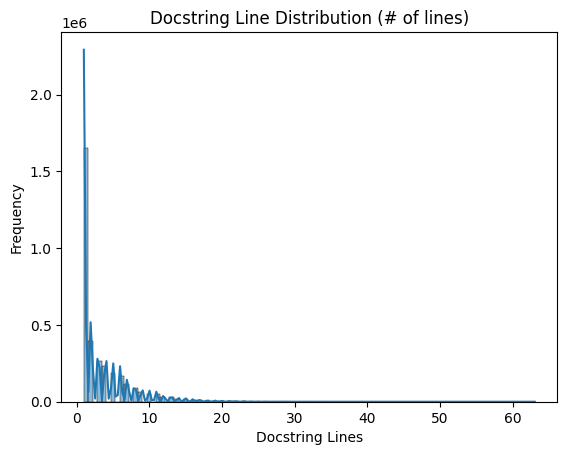
\includegraphics[width=\textwidth]{kapitel6/docline.png}
    \end{minipage}\hfill
    \begin{minipage}{0.5\textwidth}
        \centering
        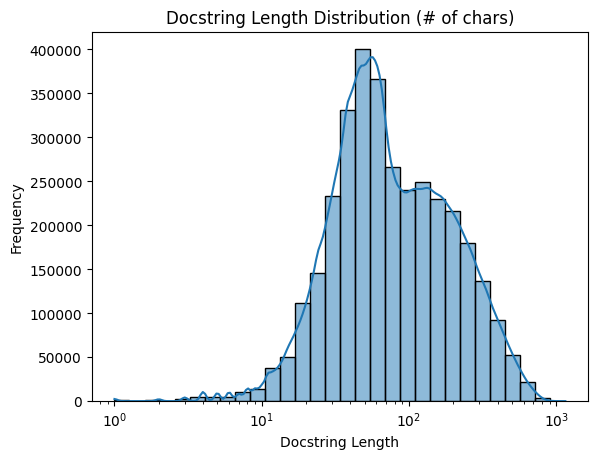
\includegraphics[width=\textwidth]{kapitel6/doclen.png}
    \end{minipage}
    \caption{Distribution of the number of docstring lines and docstring length in TinyFuncData-Python.}
    \label{fig:docdist}
\end{figure}
\end{comment}

Some of the metrics also are likely not reliable indicators of model performance.
The most concerning are MultiPL-Es PHP and Go evaluations, which produce suspiciously good results and cause occasional crashes, all of HumanEvalPack, which produced pass@1 values of zero on languages which had already provided better results on MultiPL-E, and the Leetcode Contest Benchmark, which could not be evaluated due to the lack of a proper Docker environment.
DS-1000 also provides suspiciously poor results, but this could be accurate when compared to the performance of other models.
Also, the creation of HumanEval, the basis for many of the other metrics and perhaps the most well used, is only barely mentioned in the paper where it was introduced, with a longer description in the appendix that also does not specify much about the creation process and mostly goes into detail about the properties that an evaluation set should have.

\section{Future Work}
\label{sec:future}
There is no shortage of research being done in the code synthesis \ac{llm} field, with many new advancements being made while this thesis was being written.
However, no model that this thesis is aware of fulfills the specific purpose outlined within the section \ref{sec:motivation}.
To reiterate, the research question is \emph{How well can a small \acl{lm} be fine-tuned to only synthesise function bodies from a function signature using limited hardware?}
Because no model fulfills TinyFuncCoder's use case, further research into this field is desirable to improve upon the first attempt made by the TinyFuncCoder models.

For further research, the following should be attempted or kept in mind:
TinyFuncData-Python is a solid baseline to work off of.
The evaluation metrics used, while not perfect, provide solid insight into the capabilities of a model and can be used in the future if the obsolete and non-functioning metrics are removed.
More experimentation with data structuring for training should be done.
A simple suggestion is to approach training as a natural language to code task, where the natural language docstring is seen as the input and the entire function as the output.
This was not attempted for TinyFuncCoder because the head was considered part of the input, something that the user should be able to define, but more strictly segmenting between code and language could be useful.
TinyLlama should be reevaluated as a base model, considering it did not improve much with fine-tuning on most metrics and is worse than comparable models of its size, though this could also be seen as a benefit.
While training a model from scratch might be a good solution, that prevents the use of the \ac{peft} techniques that made training possible at all.
A freshly trained model would have to be much smaller than the current 1.1 B parameters or require better hardware and more training time, and would also lack preexisting natural language and possibly code knowledge.
A good approach to try could be the recently-released \ac{qdora} \cite{Liu.2024b}, a merging of the quantization approach of \ac{qlora} and the improvements \ac{dora} \cite{Liu.2024b} makes to \ac{lora} that claims to be as resource-efficient as \ac{qlora} while improving performance to be close to full fine-tuning \cite{Liu.2024b}.
Finally, the best \ac{lm} of 1.5 B and fewer parameters that this thesis is aware of, DeepSeekCoder-1.3B-Base, achieves a pass@1 of 30\% on HumanEval.
Model size seems to be correlated to performance on this metric.
Any potential near-future work to create a TinyFuncCoder model trained from a small \ac{lm} will most likely also achieve a pass@1 of 30\% at best, making it unreliable as a coding assistant even in the best case scenario.
This is especially problematic in its intended setting, a classroom, where a less experienced student may not easily spot or understand mistakes made by the model.
\chapter{Conclusion}
\label{chap:conclusion}
This chapter serves as a summary of the work done in this thesis and the produced results.
This thesis has introduced the TinyFuncCoder series of code synthesis \acp{lm}.
This series of models was intended to be a proof of concept for a tool used in academic settings to teach students to work in tandem with a \ac{lm} when writing code.
TinyFuncCoder was intended to generate a function body from a signature, namely the docstring, function head and parameters.
The models were intended to be small so they could be run on the hardware accessible to most students and limited in their knowledge of broader programming structures like classes to encourage students to plan out a code architecture for themselves and only being able to generate one function at a time.
These models were trained under time constraints posed by the scope of a Master's thesis -- six months -- and under resource constraints -- being limited to personal hardware and a server of the University of Applied Sciences of Mannheim.
These restrictions proved to be a large challenge in training the TinyFuncCoder series.

To train the models, a custom dataset was created from The Stack dataset, a massive collection of GitHub source code files.
Function definitions of the ten most popular programming languages were extracted with custom \ac{regex}es and split into their components -- programming language, function head, body, parameters and docstring.
Docstrings were not properly extracted for all languages but Python.
TinyLlama models were chosen as the base as they are small, open-source and have decent perfomance on multiple metrics, including code knowledge for TinyLlama-v1.0.
Some exploratory training and a small hyperparameter analysis were done before proper training of the TinyFuncCoder models began.
During training, the data was split into one-percent chunks of the TinyFuncData dataset and swapped out every epoch.
During this process, and crashes during training due to memory issues, trainer and optimizer states were lost.

Ultimately, TinyFuncCoder-v1.0 is not markedly more capable than TinyLlama-v1.0 on average, improving on some metrics and worsening on others.
Its biggest success is an improvement on MultiPL-E, even on languages which it was not fine-tuned on.
TinyFuncCoder-v1.1 does not achieve any programming capabilities at all, presumably because TinyLlama-v1.1 was not pretrained on code and it was not trained on a sufficient amount of data to acquire this knowledge.
This result could be caused by many factors, including decisions and mistakes made during dataset creation and training, little hyperparameter analysis due to time and hardware constraints, the model not being trained on enough data due to time constraints, or possibly a poor choice of data formatting for training.
Taking this into consideration, TinyFuncCoder-v1.0's performance broadly matching or outperforming the TinyLlama series despite multiple setbacks during training can be seen as a success.
The main limit to the creation of a vastly more capable model remains the size, one of its key components, as model performance on the chosen metrics is tied to model size.
Further, the TinyLlama series, even the models specifically trained for coding, are also limited to similarly middling performance.
The chosen metrics, most of them commonly adopted for code synthesis evaluation, are biased towards Python and are partially unreliable.

To answer the research question posed, and for future work to take into consideration, this thesis concludes that creating a model under the given constraints is very challenging, even if all decisions had been made optimally.
A model of TinyFuncCoder's size is currently not capable of achieving a coding ability good enough to serve as a reliable coding assistant for students, especially when considering the restriction of only being able to generate functions without deeper knowledge of code structures.
A capable small coding model is certainly possible, and the research into smaller models is also progressing steadily, but such a model still requires more time and resource investment than is possible within the scope of this thesis.


\label{lastpage}
%Beginn des Anhangs. Befehl \appendix nicht entfernen auch wenn kein Anhang vorhanden ist!
\appendix

%Wenn Sie keinen Anhang haben, entfernen Sie ausschließlich die nachfolgenden beiden Dateien.
\chapter{Error Analysis}
\label{sec:error}
After the main work of this thesis was concluded, an experiment was done to judge the capability of the training architecture used in this thesis.
To see if it can achieve a very simple result, the goal was to train the model on two consecutive words -- \enquote{Hello Banana}.
Generating one word to follow the next is one the most simple tasks a \ac{lm} can be trained to do and is much, much more cheap in terms of time and resource cost than fine-tuning on a large dataset like TinyFuncData.
This allows a more elaborate hyperparameter analysis to be done on various model configurations.
The parameters and values chosen are shown in table \ref{tab:parameters}

\begin{table}[!h]
    \centering
    \caption{Possible parameter values for the fine-tuning experiments done to test the capabilities of the fine-tuning pipeline.}
    \begin{tabular}{l|r|r|r|r}
        \hline
        \textbf{Training Parameters} \\
        \hline
        \texttt{weight\_decay} & 0 & 0.1 \\
        \texttt{learning\_rate} & 1e-4 & 1e-5 \\
        \texttt{fp16} & \texttt{True} & \texttt{False} \\
        \hline
        \textbf{\ac{lora} Parameters} \\
        \hline
        \texttt{r} (rank) & 1 & 8 & 64 & 1024 \\
        \texttt{lora\_alpha} & 1 & 8 & 64 & 1024 \\
        \texttt{lora\_dropout} & 0 & 0.1 & \\
        \hline
        \textbf{\ac{qlora} Parameters} \\
        \hline
        \texttt{load\_in\_4bit} & \texttt{True} & \texttt{False} \\
        \texttt{bnb\_4bit\_use\_double\_quant} & \texttt{True} & \texttt{False} \\
        \texttt{bnb\_4bit\_compute\_dtype} & \texttt{bfloat16} & \texttt{float32} \\
        \hline
    \end{tabular}
    \label{tab:parameters}
\end{table}

TinyLlama-v1.1 is trained on all possible combinations of these parameters with full fine-tuning, using only \ac{lora} and using both \ac{lora} and \ac{qlora} for 100 epochs per training, excluding those that have no effect on the model.
For example, models that do not use \ac{qlora} do not iterate over \ac{qlora} parameters as the resulting models would all be identical.

After training, a pipeline is used to generate an output for the input \enquote{Hello}, with the expectation of recieving \enquote{Hello Banana[...]} as a response.
The pipeline is created with the \texttt{text-generation} task and generated ten new tokens.
Various states of the model are used to generate the text:
For full-parameter tuning, the model used in training is prompted directly, the model is saved and loaded back in and prompted, and the base model is loaded and prompted as a baseline check to compare to.
For \ac{lora} training, both the model from training and the model loaded from a checkpoint are prompted before and after calling \texttt{merge\_and\_unload()}, which merges the \ac{peft} parameters back into the base model.
Between each training and generation block, all of the used classes are manually deleted using Python's garbage collection library \texttt{gc} to ensure no bleedover of any kind is possible.

Analysing the resulting generations offers the following insights:
For all models, the responses are limited to the following possibilites.
The number in the bracket indicates how often this response was given.
\begin{itemize}
    \item A: \enquote{Hello$\backslash$nApril 20, 20} (2781)
    \item B: \enquote{Hello. I'm a 20-something} (1072)
    \item C: \enquote{Hello Hello Hello Hello Hello Hello Hello Hello Hello Hello Hello} (50)
    \item D: \enquote{Hello Bananaanaanaanaanaanaanaanaana} (32)
    \item E: \enquote{Hello The$\backslash$nApril 20, 2} (15)
    \item F: \enquote{Hello Banana Banana Banana Banana Banana} (12)
    \item G: \enquote{Hello The Hello Hello Hello Hello Hello Hello Hello Hello Hello} (2)
    \item H: \enquote{Hello A 2 2 2 2 } (1)
\end{itemize}
Response A is the one given by the base model.
This response is given for the baseline check of each of the model configurations without fail.
Of the other responses, only D and F can be considered a success as their generation begins with the desired string.
Training crashed after 793 models finished training.
The results of this first set of models will be explored before discussing the rest of the generations.
Of the 793 models, only twelve produced one D or F.
These are shown in table \ref{tab:banana}.

\begin{table}
    \centering
    \small
    \caption{The twelve model configurations that successfully printed \enquote{Hello Banana[\dots]} after 100 epochs of training.}
    \begin{tabular}{rrrrrrrrrr}
        \hline
        Weight & Learning & FP16 & \ac{lora} & \ac{lora} & \ac{lora} & \ac{qlora} & \ac{qlora} & \ac{qlora} \\
        Decay & Rate & & Rank & Alpha & Dropout & 4bit & Double Quant. & Type \\
        \hline
        0.1 & 1e-5 & \texttt{False} & 1024 & 1024 & 0.1 & - & - & - \\
        0.1 & 1e-5 & \texttt{False} & 1024 & 1024 & 0.0 & - & - & - \\
        0.1 & 1e-5 & \texttt{False} & 1024 & 64 & 0.0 & - & - & - \\
        0.1 & 1e-5 & \texttt{False} & 64 & 1024 & 0.1 & - & - & - \\
        0.1 & 1e-5 & \texttt{False} & 64 & 1024 & 0.0 & - & - & - \\
        0.1 & 1e-5 & \texttt{False} & 64 & 64 & 0.0 & - & - & - \\
        0.1 & 1e-5 & \texttt{False} & 8 & 1024 & 0.1 & - & - & - \\
        0.1 & 1e-5 & \texttt{False} & 8 & 1024 & 0.0 & - & - & - \\
        0.1 & 1e-5 & \texttt{False} & 1 & 1024 & 0.1 & - & - & - \\
        0.1 & 1e-5 & \texttt{False} & 1 & 1024 & 0.0 & - & - & - \\
        0.1 & 1e-5 & \texttt{False} & 1 & 64 & 0.1 & - & - & - \\
        0.1 & 1e-5 & \texttt{False} & 1 & 64 & 0.0 & - & - & - \\
        \hline
    \end{tabular}
    \label{tab:banana}
\end{table}



Table \ref{tab:generations} shows the distribution of each response per model loading variation.
\begin{table}
    \centering
    \caption{Distribution of all possible responses given by the 793 models trained on \enquote{Hello Banana} and loaded in various ways.}
    \begin{tabular}{l|rrrrrrrr}
        \hline
        Response & Direct & Merged & Loaded & Mrg.+Ld. & Base \\
        \hline
        A & 225 & 226 & 768 & 769 & 793 \\
        B & 536 & 536 & 0 & 0 & 0 \\
        C & 13 & 12 & 13 & 12 & 0 \\
        D & 8 & 8 & 8 & 8 & 0 \\
        E & 8 & 7 & 0 & 0 & 0 \\
        F & 3 & 4 & 3 & 2 & 0 \\
        G & 0 & 0 & 0 & 2 & 0 \\
        H & 0 & 0 & 1 & 0 & 0 \\
        \hline
    \end{tabular}
    \label{tab:generations}
\end{table}

The results shown in the table are concerning, as it shows that the model can produce inconsistent outputs for each variation of loading it.
The largest variation is between the direct use and loading it back in, where response B is entirely lost and becomes response A, but small variations also exist in the other responses, including the entirely unique responses G and H.
This puts into question if the knowledge that was gained during the training of TinyFuncCoder was only partially retained, or in the worst case, not at all.

What is even more concerning is that when resuming training after it crashed, almost every subsequently trained model gave at least one response which included \enquote{Hello Banana} and had a much wider range of possible responses in general.
Retraining some of the old configurations also gave different responses than before despite using a seed.
This makes the training process using \ac{lora} and \ac{qlora} very difficult to track and reproduce.
%\chapter{Zweiter Anhang: Lange Tabelle}
\label{AnhangB}

Hier ein Beispiel für einen Anhang. Der Anhang kann genauso in Kapitel und Unterkapitel unterteilt werden, wie die anderen Teile der Arbeit auch.

\sffamily
\begin{footnotesize}
  \begin{longtable}[c]{ p{.5\textwidth} p{.1\textwidth} p{.1\textwidth} p{.1\textwidth}}
    \caption[Tabelle mit ISO-Ländercodes]                       % Caption für das Tabellenverzeichnis
        {Lange Tabelle mit ISO-Ländercodes\label{laendercodes}} % Caption für die Tabelle selbst
        \\
    \toprule
    \textbf{Country} & \textbf{A 2} & \textbf{A 3} & \textbf{Number} \\
    \midrule
    AFGHANISTAN                                    & AF & AFG & 004 \\
    ALBANIA                                        & AL & ALB & 008 \\
    ALGERIA                                        & DZ & DZA & 012 \\
    AMERICAN SAMOA                                 & AS & ASM & 016 \\
    ANDORRA                                        & AD & AND & 020 \\
    ANGOLA                                         & AO & AGO & 024 \\
    ANGUILLA                                       & AI & AIA & 660 \\
    ANTARCTICA                                     & AQ & ATA & 010 \\
    ANTIGUA AND BARBUDA                            & AG & ATG & 028 \\
    ARGENTINA                                      & AR & ARG & 032 \\
    ARMENIA                                        & AM & ARM & 051 \\
    ARUBA                                          & AW & ABW & 533 \\
    AUSTRALIA                                      & AU & AUS & 036 \\
    AUSTRIA                                        & AT & AUT & 040 \\
    AZERBAIJAN                                     & AZ & AZE & 031 \\
    BAHAMAS                                        & BS & BHS & 044 \\
    BAHRAIN                                        & BH & BHR & 048 \\
    BANGLADESH                                     & BD & BGD & 050 \\
    BARBADOS                                       & BB & BRB & 052 \\
    BELARUS                                        & BY & BLR & 112 \\
    BELGIUM                                        & BE & BEL & 056 \\
    BELIZE                                         & BZ & BLZ & 084 \\
    BENIN                                          & BJ & BEN & 204 \\
    BERMUDA                                        & BM & BMU & 060 \\
    BHUTAN                                         & BT & BTN & 064 \\
    BOLIVIA                                        & BO & BOL & 068 \\
    BOSNIA AND HERZEGOWINA                         & BA & BIH & 070 \\
    BOTSWANA                                       & BW & BWA & 072 \\
    BOUVET ISLAND                                  & BV & BVT & 074 \\
    BRAZIL                                         & BR & BRA & 076 \\
    BRITISH INDIAN OCEAN TERRITORY                 & IO & IOT & 086 \\
    BRUNEI DARUSSALAM                              & BN & BRN & 096 \\
    BULGARIA                                       & BG & BGR & 100 \\
    BURKINA FASO                                   & BF & BFA & 854 \\
    BURUNDI                                        & BI & BDI & 108 \\
    CAMBODIA                                       & KH & KHM & 116 \\
    CAMEROON                                       & CM & CMR & 120 \\
    CANADA                                         & CA & CAN & 124 \\
    CAPE VERDE                                     & CV & CPV & 132 \\
    CAYMAN ISLANDS                                 & KY & CYM & 136 \\
    CENTRAL AFRICAN REPUBLIC                       & CF & CAF & 140 \\
    CHAD                                           & TD & TCD & 148 \\
    CHILE                                          & CL & CHL & 152 \\
    CHINA                                          & CN & CHN & 156 \\
    CHRISTMAS ISLAND                               & CX & CXR & 162 \\
    COCOS (KEELING) ISLANDS                        & CC & CCK & 166 \\
    COLOMBIA                                       & CO & COL & 170 \\
    COMOROS                                        & KM & COM & 174 \\
    CONGO                                          & CG & COG & 178 \\
    COOK ISLANDS                                   & CK & COK & 184 \\
    COSTA RICA                                     & CR & CRI & 188 \\
    COTE D'IVOIRE                                  & CI & CIV & 384 \\
    CROATIA (local name: Hrvatska)                 & HR & HRV & 191 \\
    CUBA                                           & CU & CUB & 192 \\
    CYPRUS                                         & CY & CYP & 196 \\
    CZECH REPUBLIC                                 & CZ & CZE & 203 \\
    DENMARK                                        & DK & DNK & 208 \\
    DJIBOUTI                                       & DJ & DJI & 262 \\
    DOMINICA                                       & DM & DMA & 212 \\
    DOMINICAN REPUBLIC                             & DO & DOM & 214 \\
    EAST TIMOR                                     & TP & TMP & 626 \\
    ECUADOR                                        & EC & ECU & 218 \\
    EGYPT                                          & EG & EGY & 818 \\
    EL SALVADOR                                    & SV & SLV & 222 \\
    EQUATORIAL GUINEA                              & GQ & GNQ & 226 \\
    ERITREA                                        & ER & ERI & 232 \\
    ESTONIA                                        & EE & EST & 233 \\
    ETHIOPIA                                       & ET & ETH & 210 \\
    FALKLAND ISLANDS (MALVINAS)                    & FK & FLK & 238 \\
    FAROE ISLANDS                                  & FO & FRO & 234 \\
    FIJI                                           & FJ & FJI & 242 \\
    \bottomrule
  \end{longtable}
\end{footnotesize}
\rmfamily


\textit{Beachten Sie, dass die Tabelle manchmal erst nach dreimaligem Lauf durch \LaTeX richtig angezeigt wird.}



\end{document}

